\NeedsTeXFormat{LaTeX2e}

%%%
\documentclass[12pt,a4paper]{article}
%\documentclass[12pt, a4paper]{report}

\usepackage[includeheadfoot,margin=2.5cm]{geometry}
\usepackage{amssymb}
\usepackage{amsmath}
\usepackage{floatflt}
\usepackage{graphicx}
\usepackage{color}
\usepackage{subfig}
\usepackage[ngerman,english]{babel}
\usepackage{listings}
\usepackage{url}
\usepackage[T1]{fontenc}
\usepackage[utf8]{inputenc}
\usepackage{endnotes}
\usepackage{parskip}
\usepackage{sidecap}

\usepackage{setspace}
\onehalfspacing

\usepackage[font=footnotesize]{caption}

\usepackage[
colorlinks,
pdfpagelabels,
pdfstartview = FitH,
bookmarksopen = true,
bookmarksnumbered = true,
linkcolor = black,
plainpages = false,
hypertexnames = false,
citecolor = black] {hyperref}

%%%
%\usepackage{titlesec}

%\usepackage{uarial}
%\renewcommand{\familydefault}{\sfdefault}

\usepackage[authordate,bibencoding=auto,strict]{biblatex-chicago} 
\usepackage[babel,german=guillemets]{csquotes}
\bibliography{Bibliography}

%%%
%\titleformat{\chapter}
%{\normalfont\LARGE\bfseries}{\thechapter.}{0.5em}{}

\definecolor{mygray}{gray}{.75}
\definecolor{myblue}{rgb}{.2,.3,.7}
\definecolor{myorange}{rgb}{.6,.5,.1}

\lstdefinelanguage{JavaScript}{
  keywords={typeof, new, true, false, catch, function, return, null, catch, switch, var, if, in, while, do, else, case, break },
  ndkeywords={class, export, boolean, throw, implements, import, this, window, document, \$, console, Math, navigator},
  identifierstyle=\color{black},
	showstringspaces=false,
  sensitive=false,
  comment=[l]{//},
  morecomment=[s]{/*}{*/},
  commentstyle=\color{mygray}\ttfamily,
  stringstyle=\color{black}\ttfamily,
  morestring=[b]',
  morestring=[b]"
}

\lstset{ 
  language=Matlab,
	basicstyle=\fontsize{10pt}{12pt}\selectfont\ttfamily,
	keywordstyle=\color{black},
  ndkeywordstyle=\color{black}\ttfamily,
	commentstyle=\color{mygray},
	tabsize=1,
	numbers=left,
	numberstyle=\tiny\color{mygray},
	numbersep=7pt,
	frame=tb,
  xleftmargin=15pt,
	aboveskip=20pt,
	captionpos=b,
	breaklines=true,   
  breakatwhitespace=false,
	rulecolor=\color{mygray} 
%	morekeywords={*,auto}
}

%\setcounter{tocdepth}{4}   % Aufnahme von paragraph in das Inhaltsverzeichnis
%\setcounter{secnumdepth}{4}   %Nummerierung vertiefen

%\setcounter{tocdepth}{2} 
%\setcounter{secnumdepth}{3} 

%\selectlanguage{ngerman}
\selectlanguage{english}
\renewcommand*\rmdefault{phv}

\pdfimageresolution=150
%\setlength{\parindent}{0pt}
%\setlength{\parskip}{50pt plus 20pt minus 10pt}


\begin{document}

\begin{titlepage}

\begin{center}
\Huge{ 
	\textbf{Master Thesis}
}
\end{center}

\newpage

\thispagestyle{empty}

\hfill 
\includegraphics[height=1.5cm]{images/FHSLogo.png}

\vspace*{2cm}

\Large{
DRUM SOUND ANALYSIS

Recognition and Differentiation of Drum Sounds as Extension to the E-Learning Platform Easydrum

\vspace*{1cm}

%Masterarbeit zur Erlangung des akademischen Grades
%:Master thesis to acquire the degree
Master's thesis submitted in fulfillment of the requirements for the degree
\vspace*{0.5cm}

\textit{Master of Science}
}


\vspace*{1.5cm}
{\large
%VerfasserIn: Katrin Hewer
Author: Katrin Hewer
}
\vfill

{\normalsize
%Vorgelegt am FH-Masterstudiengang MultiMediaTechnology, Fachhochschule Salzburg
Submitted at the Master's degree course in MultiMediaTechnology at Fachhochschule Salzburg, University of Applied Science

\vspace*{1cm}

Supervised by:
Assoc.-Prof. Dipl.-Ing. Dr. Rade Kutil

\vfill

%Ort, Abgabe-Datum
Salzburg, June 1, 2015
}
\end{titlepage}


\pagestyle{headings}
\pagenumbering{roman}

\subsection*{Eidesstattliche Erklärung}

Hiermit versichere ich, Vorname Familienname, geboren am 17.01.1987 in Saarbrücken, dass ich die Grundsätze wissenschaftlichen Arbeitens nach bestem Wissen und Gewissen eingehalten habe und die vorliegende Masterarbeit von mir selbstständig verfasst wurde. Zur Erstellung wurden von mir keine anderen als die angegebenen Quellen und Hilfsmittel verwendet. 

Ich versichere, dass ich die Masterarbeit weder im In- noch Ausland bisher in irgendeiner Form als Prüfungsarbeit vorgelegt habe und dass diese Arbeit mit der den BegutachterInnen vorgelegten Arbeit übereinstimmt.


\vspace*{3cm}

Salzburg, am 01.06.2015


\hfill


Unterschrift

\vspace*{1cm}

$\overline{\text{Vorname Familienname}}$ \hfill	$\overline{\text{Personenkennzeichen}}$



\newpage
\selectlanguage{ngerman}

\section*{Kurzfassung}
\vspace{0.5cm}

\begin{sloppypar}
Im Rahmen dieser Arbeit wird ein Konzept für eine Erweiterung der Online-Schlagzeugschule Easydrum vorgestellt. Das Ziel der Arbeit ist es, ein System zu erarbeiten, das die Verwendung eines analogen Schlagzeuges mit der Platform erlaubt. Dieses System hat über einen Webbrowser Zugriff auf ein mit dem Computer verbundenes Mikrofon und kann so Schlagzeugsound auslesen. Es erkennt Schläge auf Trommeln und Becken eines zuvor konfigurierten Drumsets in Echtzeit und unterscheidet diese voneinander. Um dies zu ermöglichen werden ein Onset-Detection-Algorithmus basierend auf dem Zeitbereich eines Audiosignals, sowie zwei unterschiedliche Ansätze zur Klassifizierung entwickelt. Die Algorithmen werden mithilfe von Matlab\textsuperscript{\textregistered} und Weka getestet. 
\end{sloppypar}

Der erste Ansatz für die Klassifizierung basiert auf dem Extrahieren eines Featurevektors, der dazu genutzt wird einen Decision Tree mit dem J48-Algorithmus aufzubauen. 

Im zweiten Ansatz werden zu jedem trainierten Schlagtyp zwei Templates erstellt, wobei eines das minimale und eines das maximale Frequenzspektrum des Schlages abbildet. Durch einen Vergleich der Spektralform dieser Templates mit dem Spektrum einer neuen Dateninstanz kann ein Klassenlabel für die neue Dateninstanz bestimmt werden. Die Methode wird sowohl mit einzelnen Schlägen als auch mit zwei gleichzeitigen Schlägen getestet. 

Des Weiteren gibt diese Arbeit einen Einblick in die Web Midi API, die zur späteren Umsetzung des Systems benötigt wird. Es wird ein Beispielprogramm vorgestellt, das über den Browser einen Audiostream erhält und diesen auf ein HTML Canvas-Element zeichnet.

\paragraph{Schlagwörter:}
\textit{Audiosignalverarbeitung, Signalverarbeitung, Klassifizierung, Decision Tree, J48, Onset Detection, Web Audio API, MatLab, Echtzeit}



\selectlanguage{english}

\newpage
%\selectlanguage{english}
\subsection*{Abstract}
\vspace{0.5cm}

This thesis describes the concept for an extension of the online drum school Easydrum. The aim of this thesis is to provide a system that allows to use an analog drum set with the Easydrum platform. This system is able to receive the sound of the drum set on a web browser by using a microphone. It detects strokes on drums and cymbals of a pre-configured drum kit in real-time and differentiates them from each other. Therefore, an onset detection algorithm based on the time domain of the incoming audio stream is developed and two different approaches for classification are tested. The algorithms are tested with Matlab\textsuperscript{\textregistered} and Weka. 

The first classification approach is based on the extraction of a feature vector that is used to build a decision tree with the J48 algorithm. 

In the second approach templates of the minimum and maximum frequency spectrum of each trained stroke type are created. By analyzing correlations in the spectral shapes between these templates and an unseen data instance, a class label for the unseen instance can be determined. The method is tested with single strokes as well as with two simultaneously played strokes. 

Furthermore, this thesis gives an introduction to the Web Midi API, which is required to develop the further application. An example for receiving an audio stream on the browser and displaying it on a HTML canvas element is given.

\paragraph{Keywords:}
\textit{audio signal processing, signal processing, classification, decision tree, J48, onset detection, Web Audio API, MatLab, percussive sound, real-time}

%\selectlanguage{ngerman}


\newpage
\tableofcontents

\newpage
\setcounter{page}{1}
\pagenumbering{arabic}

\newpage
\section{Introduction}
% Erl�uterung und Begr�ndung der Themenstellung (Argumentationsphase - Einleitung)
% In dieser Phase der Arbeit soll dargestellt werden, aus welchen Gr�nden das Thema der Arbeit bzw. die Forschungsfrage relevant ist bzw. wieso das Thema behandelt werden soll. Die Motivation zum Thema steht also im Vordergrund, wobei aber nicht pers�nliche Vorlieben, sondern die fachliche Wertigkeit der Fragestellung im Forschungs- und Innovationskontext gemeint ist.

The number of interactive applications has risen rapidly since the computational power of personal computers started increasing. New technologies emerge, like motion sensors and controller to interact with a software. With this development, the number of interactive applications built around sound detection and classification is growing as well. Examples for successful applications are apps that match recorded music with the respective song title and artist, or karaoke games that recognize how well the singer strikes the notes and texts. Furthermore, the broadband of the Internet and thus the performance of web-services are still making substantial progress. Ever since, new web technologies are developing that enable the web to become more and more interactive. This also leads to plenty of e-learning websites, which are readily accepted by a large audience. In particular, language learning platforms and platforms to playfully support kids in learning the alphabet or solving maths problems became quite famous in the past few years. This master's thesis makes use of the modern web technologies in order to add a high rate of interaction to the web. 

This work is based on the online e-learning platform Easydrum. It empowers its users to learn how to play drums online. The platform provides different drum lessons and exercises that can be played with an e-drum set connected to the computer. Every played drum or cymbal is displayed as its note on the sheet, which is moving over the screen during practicing. Thus, the user receives feedback on his performance. The disadvantage of the platform is that one has to use an e-drum set in order to receive feedback. A much more effective way to teach drums would be using an analog drum set. Playing with an e-drum set creates a different feeling and is not recommended by most musicians. Therefore, the aim of this master's thesis is to allow the use of an acoustic drum set with Easydrum. In order to achieve this, an algorithm that is able to recognize and analyze the sounds of drums and cymbals has been developed. The algorithm has to trigger an event to the platform when a drum or cymbal is played. This event must contain the point in time and the type of the performed stroke. With the help of this information the existing Easydrum application can create the feedback for the user.

To fully exploit the potential of Easydrum, the developed algorithm needs to fulfill several properties. The first and most important property is that the future software runs in real-time on the web with the help of JavaScript and the Web Audio API. It must detect and classify any stroke on a drum or cymbal and it has to be able to deal with multiple drum set components played at the same time. Furthermore, background music or noises can occur, which have to be filtered out. This master's thesis is focused on the real-time detection of onsets and the classification of separately stroked drums and cymbals. It further introduces an approach to the classification of simultaneously played strokes. Finally, a sample application running with the Web Audio API in the browser is presented.

%alThere is developed a drum configurator and a drum sound detector. The drum sound detector consists of an onset detector, an feature extractor and a classifier. The configurator is a training system, which is used to extract and save the features of every drum of a drum set. The user has to play every drum ten times to train this system. Afterward, the resulting training data can be used by the drum sound detector to classify played drums in real-time. The components are implemented in MATLAB.

There has already been a lot of research on similar subjects in the past. Automatic detection and classification of drum sounds have been studied in the context of music information retrieval for numerous purposes, including metrical analysis, database labeling and searches, automatic transcription, and interactive musical systems. An early work was introduced in 1994 by a paper of Goto and Muraoka \autocite[]{Goto:1994}. Their system deals with drum transcription used as a support in an audio-based real-time beat tracking system. M. Goto continued this work and developed an audio-based real-time beat tracking system for music with or without drum-sounds \autocite[]{Goto:2001}. This research is an important basic for every following work in the field of beat tracking and drum transcription. A work similar to the approach of this thesis was written by students of the Aalborg University in 2007. It deals with the automated recognition of drum types \autocite[]{Christophersen:2007}. Audio files with drum sounds are analyzed and transcribed to a readable format. The resulting algorithm can distinguish between a kick drum, a snare drum and a hi-hat. It is divided into onset detection, feature extraction and classification. The significant distinction to this thesis is that their system does not support real-time and cannot recognize cymbals. Another difference is that their algorithm does not require a training system. The configuration of a drum kit by a training system facilitate the recognition of played strokes. For the real-time part of the developed algorithm a paper published in 2010, which deals with real-time automatic detection and labeling of percussive sounds for interactive systems \autocite{Simsekli:2011}, has been considered. This paper introduces a model-based algorithm for the detection of percussive events. The model is trained offline with different percussive sounds by creating spectral templates for each sound. To detect and classify sounds from an audio stream input, a Hidden Markov Model is used. The classification is able to run online. An interesting approach to onset detection, with regard to real-time, is the doctor's thesis from W. Andrew Schloss from 1985 \autocite[]{Schloss:1985}. Schloss describes an easy algorithm on the automatic transcription of percussive music. Whereas most state of the art onset detection algorithms analyze the frequency spectrum of a recording, he only considers the amplitudes in the given acoustic waveform. With this approach, the algorithm reaches a low run time. Based on this research, this thesis presents different approaches to onset detection and classification. 

As a first step, an onset detection algorithm is developed based on the method introduced by \autocite{Schloss:1985}. This algorithm is tested with 18 different short recordings containing a total number of 226 onsets. The onsets include single strokes of each tested drum and cymbal as well as simultaneously played strokes. Out of all 226 onsets, 225 onsets were detected correctly and only on false positive onset was detected. 

After the onset detection, the thesis presents two different approaches for classification of the components of a standard drum kit. A training method is developed that ensures the usability of the aimed software by reducing the number of training instances to one stroke per stroke type. Both methods are tested with ten class labels including 29 different stroke types. For each stroke type ten test instances are recorded. Thus, the test set contains a total number of 290 instances. The second method is also tested with simultaneous strokes. Therefore, an additional test set of 120 instances is created. It contains combinations of two different drums, two different cymbals or a drum and a cymbal. The first method for classification uses a J48 decision tree. The tree is built by applying a feature vector of each stroke type that contains different values extracted from the frequency spectrum of the strokes. The method is tested with different feature sets. The best results are gained with a small feature set of three different features. A hit-rate of 91.72 \% is reached with this approach. The second approach is a template-based method. It also considers the frequency spectra of the different stroke types. There are constructed templates for the minimum and maximum amplitudes in the spectra of each stroke. Based on these templates, the spectral shape of unseen data instances is compared with the templates of each trained stroke type and classified as the most similar one. With this method a hit-rate of 97.2 \% is reached. If there are only considered drums (excluding cymbals), even a hit-rate of 100 \% is reached. The method can also distinguish between different stroke positions on the same drum. 70.3 \% of the tested instances are classified with the correct stroke type. For multiple strokes played at once a hit-rate of 81.67 \% is reached.

Finally, this thesis introduces a sample web application that uses JavaScript and the Web Audio API to receive an audio stream from a connected microphone. It animates the incoming audio wave on an HTML canvas element. This basic application can be extended by the developed onset detector and classification algorithm. Thus it builds a basis for the further implementation of the extension for the online platform Easydrum.

In the following sections of this thesis the development of the previously mentioned algorithms and application is described in detail. First, chapter \ref{section:basicConcepts} gives a short introduction to basic concepts needed for the development of the different algorithms. At this point, the platform Easydrum is introduced and a basic concepts of the components and notation of drum sets are given. This chapter also explains the basics of audio processing, including the digitization of sound and the transformation to its frequency spectrum. Finally, the basic concepts of onset detection and classification as well as the used development and testing tools MatLab\textsuperscript{\textregistered} and Weka, are introduced. In chapter \ref{section:relatedWork} different existing papers related to onset detection and classification of drum sound are presented. The chapter focuses on the onset detection algorithm in \autocite{Schloss:1985}, the classification methods of \autocite{Christophersen:2007}, \autocite{Bello:2005}, and the real-time approach in \autocite{Simsekli:2011}. The developed methods and the appropriate test results are described in detail in chapter \ref{section:methods}. First, in section \ref{section:hardware}, the used test drum set and hardware is specified. After that, in section \ref{section:onsetdetectionmethod}, the recordings for the onset detection are described and analyzed. Additionally, the developed onset detection algorithm and its test results are discussed. In section \ref{section:classificationSpectrumAnalysis} the frequency spectra of the different used drums and cymbals are analyzed. In the sections \ref{section:training} and \ref{section:testset} the creation of training and test set is described. The methods developed for classification are focused in sections \ref{section:method1} to \ref{section:methodCombined}. The received results are summarized and analyzed. After that, the sample JavaScript application is explained in section \ref{section:methodJavascript}. Finally, in chapter \ref{section:conclusion}, the results of all tested methods are summarized and discussed. The chapter also gives an outlook to further steps required to develop the final extension for Easydrum.
\newpage
\section{Basic Concepts}
\label{section:basicConcepts}
% Darstellung des aktuellen Wissens zum Thema (Literaturphase – Grundlagen)
% Hier ist ein Überblick über das Fachthema und die Begrifflichkeiten sowie eine Darstellung bestehender Lösungsansätze/Technologien anhand von Quellen aus der wissenschaftlich-technischen Literatur zu erarbeiten. Besonderes Augenmerk ist auf die korrekte Zitierweise von Quellen zu legen. Anderen LeserInnen der Arbeit soll damit das Verständnis für die darauf folgenden Teile der Arbeit erschlossen werden. Inhalte flüchtiger Quellen (Websites) sind geeignet, müssen aber gesichert werden (CD/DVD).

% zusammenfassung aller themen einfügen 
In this chapter, the existing web platform Easydrum and its technologies gets introduced, as well as the concepts of a drum set and its notation. Subsequently, an overview to audio signal processing, onset detection, different methods for classification and the Web Audio API is given. Thereby, the features and technologies required for the methods developed in this thesis can get pointed out which.

\subsection{Easydrum} \label{section:Easydrum}

\begin{figure}[ht]
	\centering
	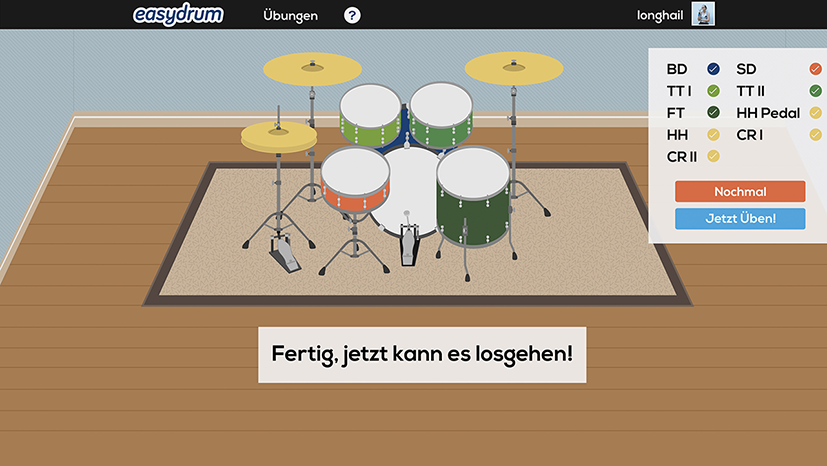
\includegraphics[width=\textwidth]{images/Easydrum/configuratorscreen.png}
	\caption{Easydrum drum configurator.}
	\label{fig:configuratorscreen}
\end{figure}

Easydrum is a free e-learning platform on the web. It provides a couple of different exercises for learning how to play a drum set. The user gets an introduction to the different components of the drum set and learns to read drum sheets. What makes the platform unique is the possibility to connect an e-drum set to it via USB to play the exercises. After connecting, the MIDI signals produced by the e-drum set can be read and processed by the platform. This way, giving feedback to the user during playing an exercise is facilitated. Before the e-drums can be used for exercising, they have to be configured with the provided e-drum configurator. Here, the user has to play each drum once to save the appropriate MIDI signal. In addition to an e-drum set, the computer keyboard can be used for exercising as well.

The application displays the exercises as drum sheets. When the exercise started, the notes are moving over the sheet. A highlighted hit area on the sheet shows the point in time when a note needs to be played. Further on, an illustration of a drum set animates the exercise while playing it. By using a configured e-drum set or the computer keyboard, the application can recognize if the right drums are stroked at the right time. The played notes are added to the sheets in real-time to show the user if he hit or missed a note. After the exercise is finished, the user gets rewarded with zero to 100 points and zero to three stars, depending on the hit-rate.

\begin{figure}[ht]
	\centering
	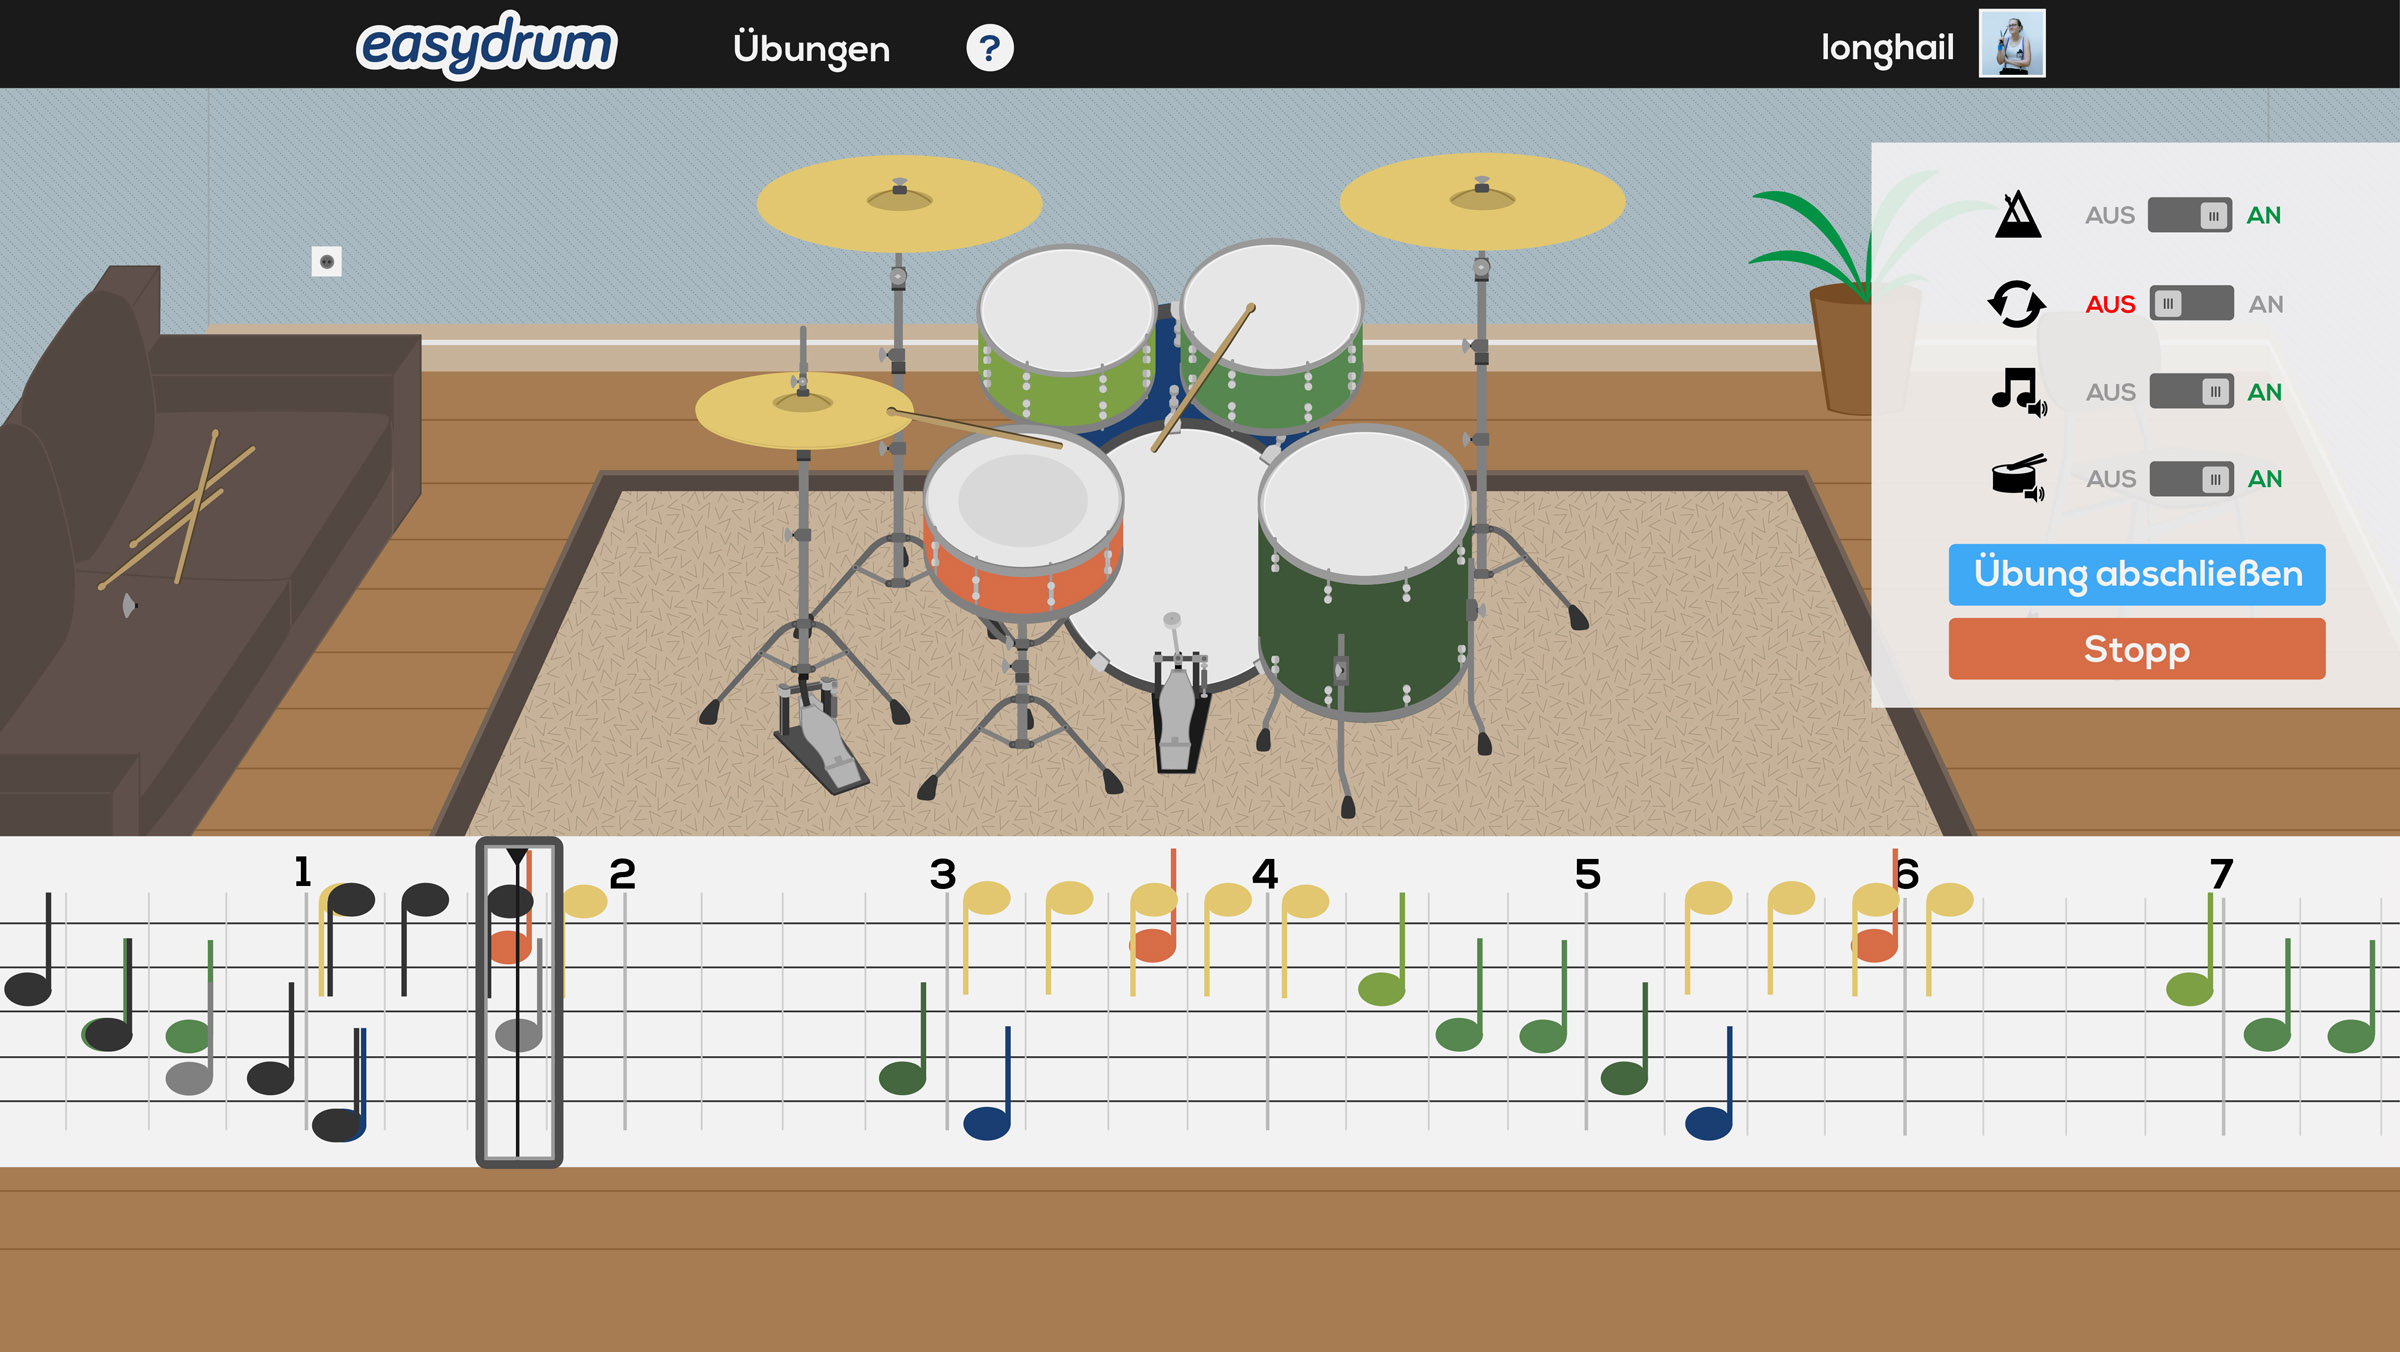
\includegraphics[width=\textwidth]{images/Easydrum/exerciseplayerscreen.png}
	\caption{Easydrum exercise player.}
	\label{fig:exerciseplayerscreen}
\end{figure}

The application is build on the open-source web framework Ruby on Rails. An overview to the framework is given on their web site \autocite{RubyOnRails:2015}. For this thesis two components of the web site are important for a detailed analysis. The e-drum configurator on the one hand and the exercise player on the other hand. Screenshots of the existing drum configurator and exercise player are shown in figures \ref{fig:configuratorscreen} and \ref{fig:exerciseplayerscreen}. 


\newpage
\newpage

\subsubsection{Technologies}
The components of Easydrum largely run in the web frontend with the help of JavaScript. 

JavaScript is a scripting language published in 1995 to supplement HTML and thus enable easy interactions with the Netscape Navigator browser. The language developed quickly from an easy scripting language to a widely used standard in web applications. It has been documented under the ECMAScript standard by the Ecma International organization. Today, JavaScript runs in all major browsers and thus enables the development of modern interactive web applications, which can run on the web frontend with high performance. Current browsers support ECMAScript 5, whereas a sixth version already exists and will be adopted to browsers, in the future. A detailed introduction to JavaScript can be found in \autocite{Haverbeke:2014}.

In addition to JavaScript, Easydrum uses jQuery and the jQuery UI widget factory. According to the jQuery web site \autocite{jQuery:2015}, jQuery is `a fast, small, and feature-rich JavaScript library. It makes things like HTML document traversal and manipulation, event handling, animation, and Ajax much simpler with an easy-to-use API that works across a multitude of browsers'. The jQuery UI widget factory provides a framework that enables developers to write stateful jQuery plug-ins, so-called widgets. It provides object oriented methods to manage the life cycle of a widget, which includes creating and destroying a widget, changing options, making super calls and receive event notifications. The jQuery UI widget factory is documented in \autocite{jQueryUI:2015}.

The key feature in the existing application is the method for receiving MIDI events from the connected e-drum set. Therefore, Easydrum uses the Web MIDI API, which is supporting the MIDI protocol. It enables web applications to communicate with MIDI input and output devices. The Web MIDI API specification was published by the W3C Audio Working Group as a Working Draft \autocite{WebMidiApi:2015}. Thus, it is not yet an official web standard and it is also not yet implemented in all common browsers but is intended to become a standard. The actual Easydrum application is able to run without an additional plug-in in Google Chrome. For other browsers the Jazz-Plugin \autocite{JazzPlugin:2015} has to be installed to receive MIDI input. As soon as the Web MIDI API is accessible via the other browsers, the plug-in will no longer be needed. 

\subsubsection{Architecture}

The basic architecture of the Easydrum application is show in figure \ref{fig:Easydrumarchitecture}. As mentioned before, the player largely runs in the web frontend with the help of JavaScript and the jQuery UI widget factory. 

\begin{figure}[ht]
	\centering
	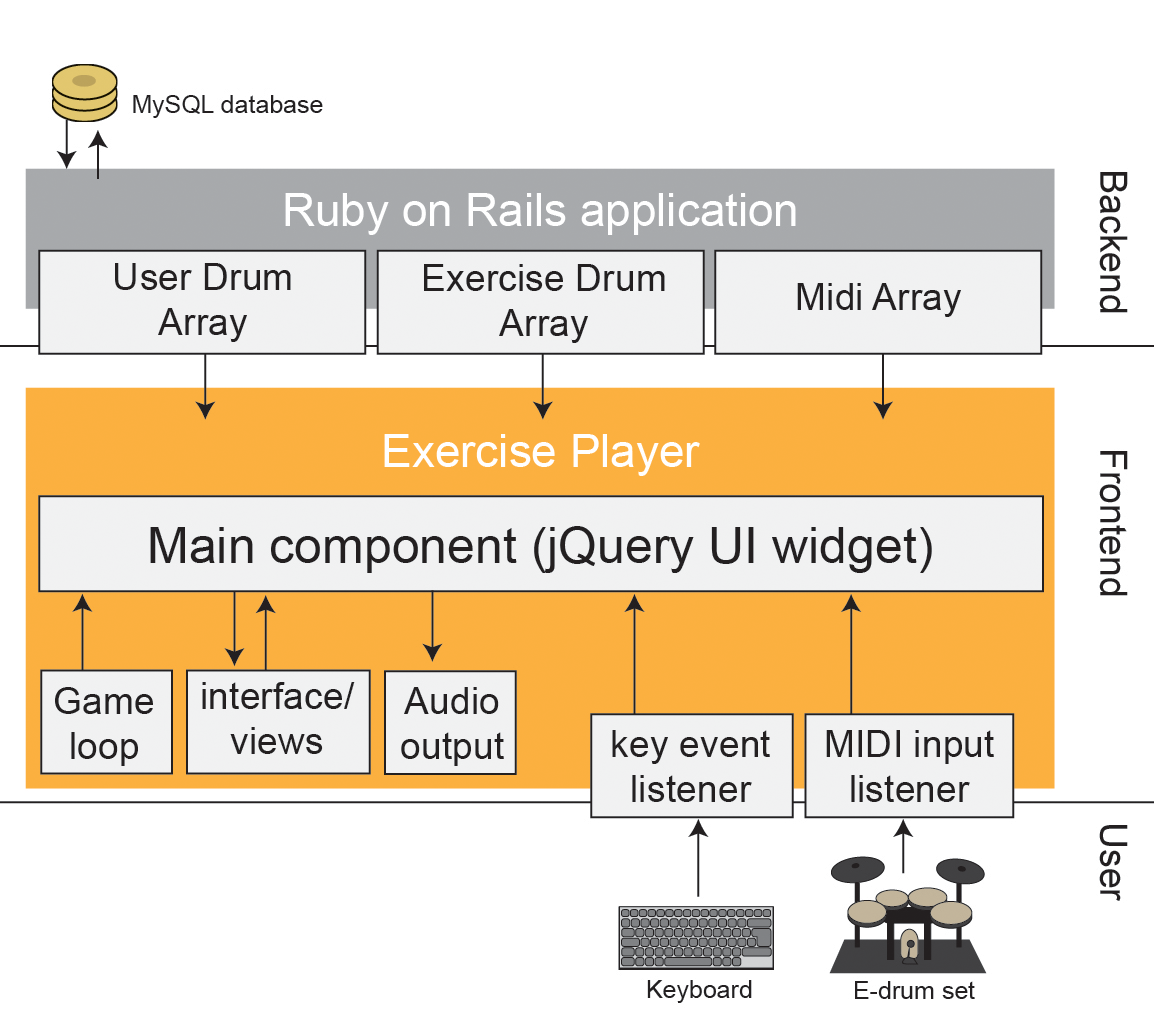
\includegraphics[width=.8\textwidth]{images/Easydrum/app_architcture.png}
	\caption{Easydrum application architecture.}
	\label{fig:Easydrumarchitecture}
\end{figure}

One main jQuery UI widget connects all components of the player. These components are the game loop, the views, two input listeners and the audio output. Each event in one of these components is sent to the main widget. The main widget processes all events and subsequently updates the relevant components. If an exercise is playing, the game loop adjusts the number of frames per seconds depending on the calculation power of the used computer. It invokes an event called \textit{tick} for every frame.

The main widget needs three arrays to be initialized. The first two arrays contain data for an e-drum set. They define the MIDI data mapped to appropriate drums. One of the drum arrays contains the data for the e-drum set used to record the exercise, the other contains the data for the drum set of the actual user. The third array contains the MIDI data that describe the actual exercise.

The input data is received by the two listeners. There is one listener that is able to receive MIDI data and one that is able to receive key events from the computer keyboard. These listeners are initialized with the user drum array described in the preceding. With the help of this array the input is mapped to the played drum and note. For every played drum the note value and the point in time when it was played is saved.

Hence, to extend the application to work with an acoustic drum set, a new listener, which maps audio input to played drums, needs to be developed and appended to the main widget.

\subsection{Components of a Drum Set}

The developed Easydrum extension receives audio data from an analog drum set. To understand these methods, the instrument and its components are introduced below.

\begin{figure}[htb]
	\centering
	\subfloat[1 - hi-hat, 2 - snare drum, 3 - bass drum 4 - tom 1, 5 - tom 2, 6 - tom 3,  7 - crash cymbal, 8 - ride cymbal]{
		\includegraphics[height=6.0cm]{images/drumset/drumset_02.jpg}
		\label{fig:components}
	}
	\qquad
	\subfloat[Rim, bow and bell of a cymbal.]{
		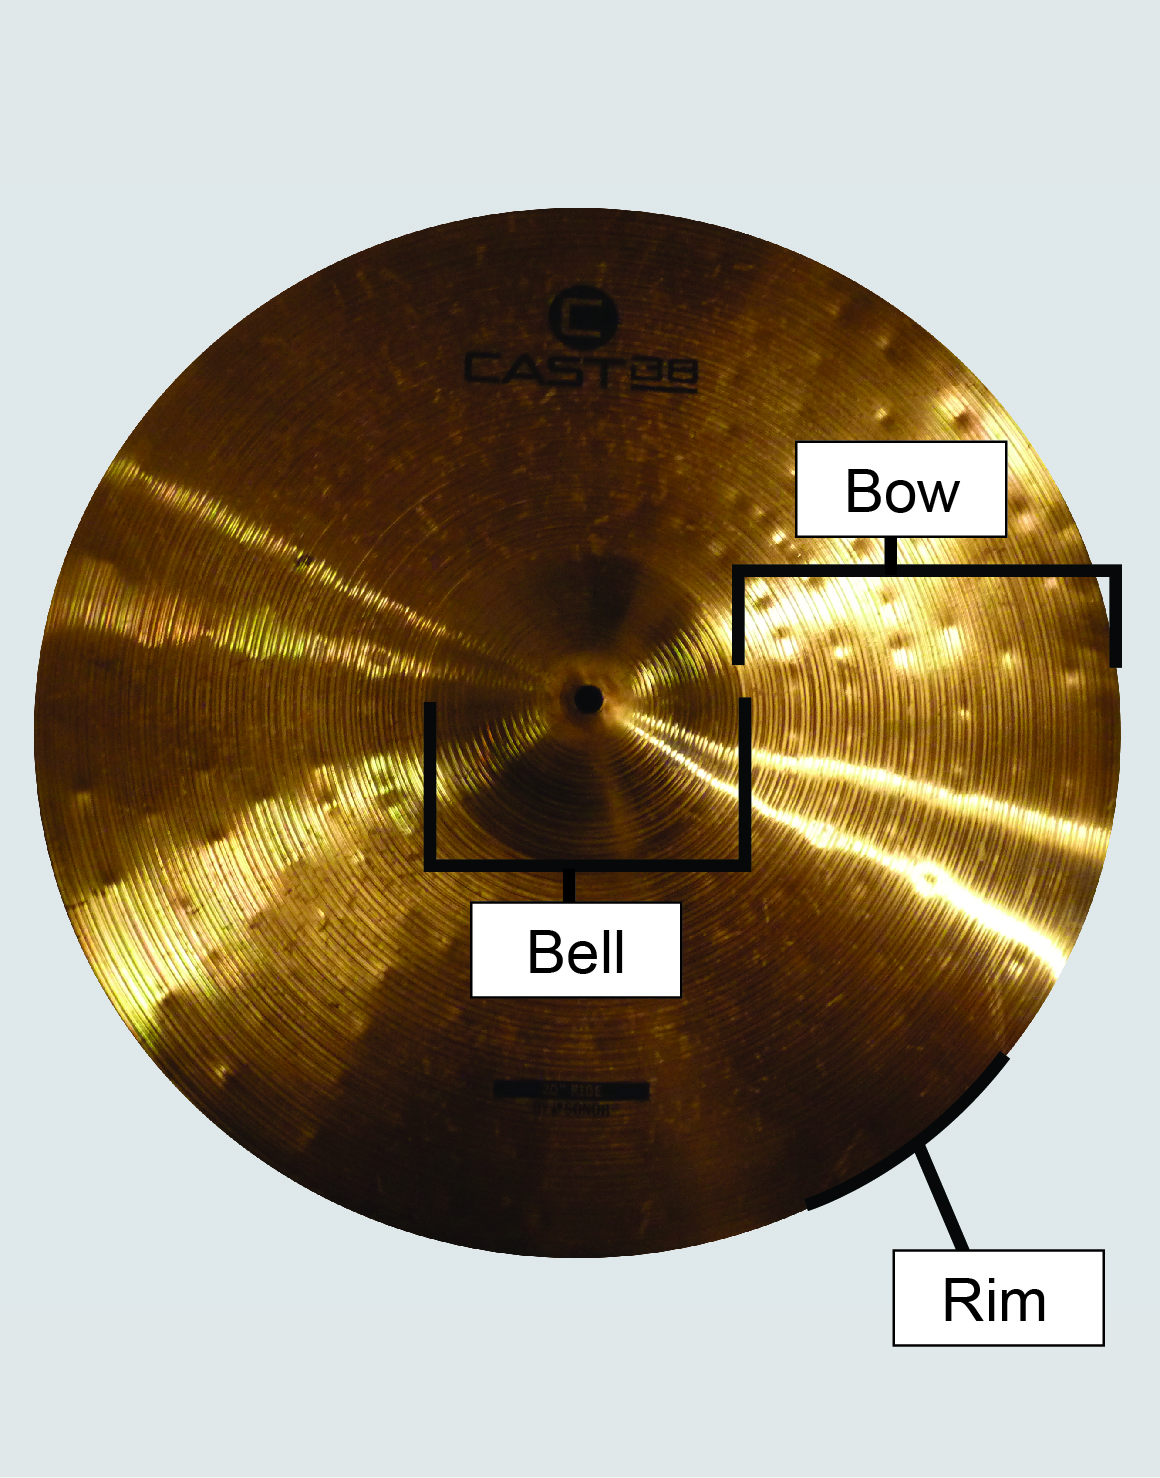
\includegraphics[height=6.0cm]{images/drumset/ride.jpg}
		%for reference of this subfigure only
		\label{fig:rim_bow_bell}
	}
	\caption{
		Components of a standard drum set.
	}
	\label{fig:drumset}
\end{figure}

A drum set is a percussive instrument. Percussive instruments are one of the oldest types of instruments in history. Today, a wide range of different instruments of this type have been created. Thus, a drum set can consist of various numbers of different drums, cymbals and other components, such as woodblocks, bells and triangles. To limit the possibilities, this thesis merely uses a standard drum set.

A standard drum set, as displayed in figure \ref{fig:components}, consists of eight different drums, which are a bass drum, a snare drum, two rack toms, a floor tom, a hi-hat, a ride cymbal and a crash cymbal. The bass drum is the central element of the drum set. Strokes are made with the help of a foot pedal. Together with the hi-hat and the snare drum, the bass drum defines the rhythm of a piece of music. The hi-hat consists of two cymbals that can be closed by a foot pedal. Thus, it can be played either opened or closed. The toms and cymbals are primarily used to play fill-ins\footnote{musical phrases between melody or song segments} and accents. As shown in figure \ref{fig:rim_bow_bell}, the cymbals consist of three components which create different sounds. These are the rim, the bow and the bell, whereas the rim is the utter part of the cymbal, the bell is a bulge in the center of it and the bow is the area on the top between the rim and the bell.


\subsection{Notation}

Typically, sheets are used to visualize a drum rhythm. Thus, in this thesis, drum sheets are used to visualize the tested drum rhythms in section \ref{section:onsetdetectionmethod}. To understand these sheets, the drum notation is explained in the following.

A sheet contains different elements like staff, clef, notes, pauses and bars, which are used to build a rhythm. A sample sheet is shown in figure \ref{fig:sheetExample}.

\begin{figure}[h]
	\centering
	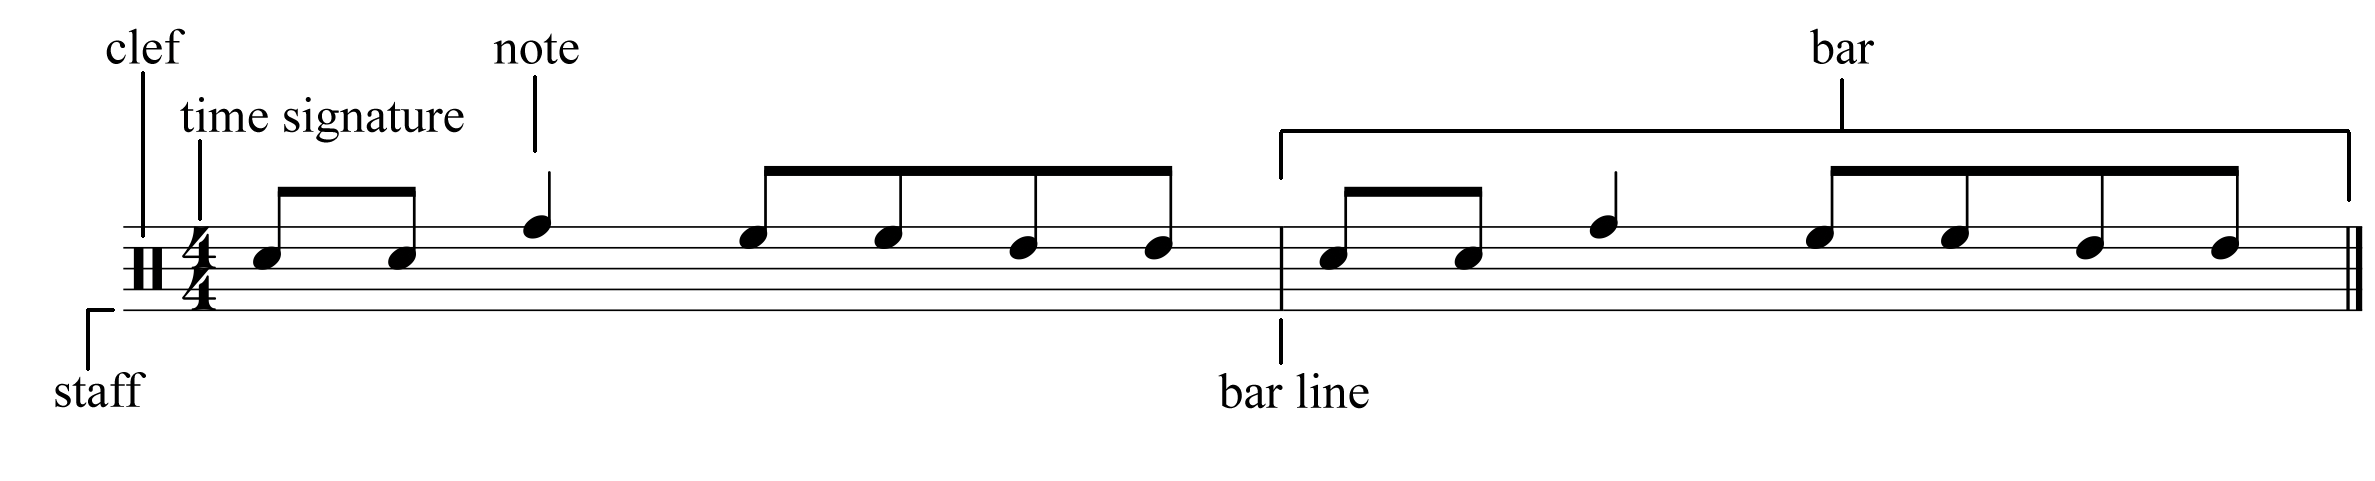
\includegraphics[width=\textwidth]{images/drumsandsheets/example.png}
	\caption{Example drum sheet.}
	\label{fig:sheetExample}
\end{figure}

The staffs are the horizontal lines on which the notes are placed. A sheet contains five staffs. 

The meaning of the particular notes is defined by the used clef. The clef is placed at the beginning of each sheet. Common clefs are for example the treble clef or the bass clef. A neutral clef is used for drum sets. In contrast to the notation of most clefs, the position of a note on the staff does not indicate its pitch, but symbolizes the component of the used drum kit that has to be stroked. Thereby, different notations are used for drum sets. Hence, to explain which note symbolizes which drum, a so called 'drum key' is used. Generally, round note heads are used for drums and x-shaped ones for cymbals. If a stroke is performed by a stick, the stem of the appropriate note is placed from the note head upwards and if it is performed with a foot pedal from the note head downwards. For this thesis, the drum key shown in figure \ref{fig:sheetNotation} is used.

\begin{figure}[h]
	\centering
	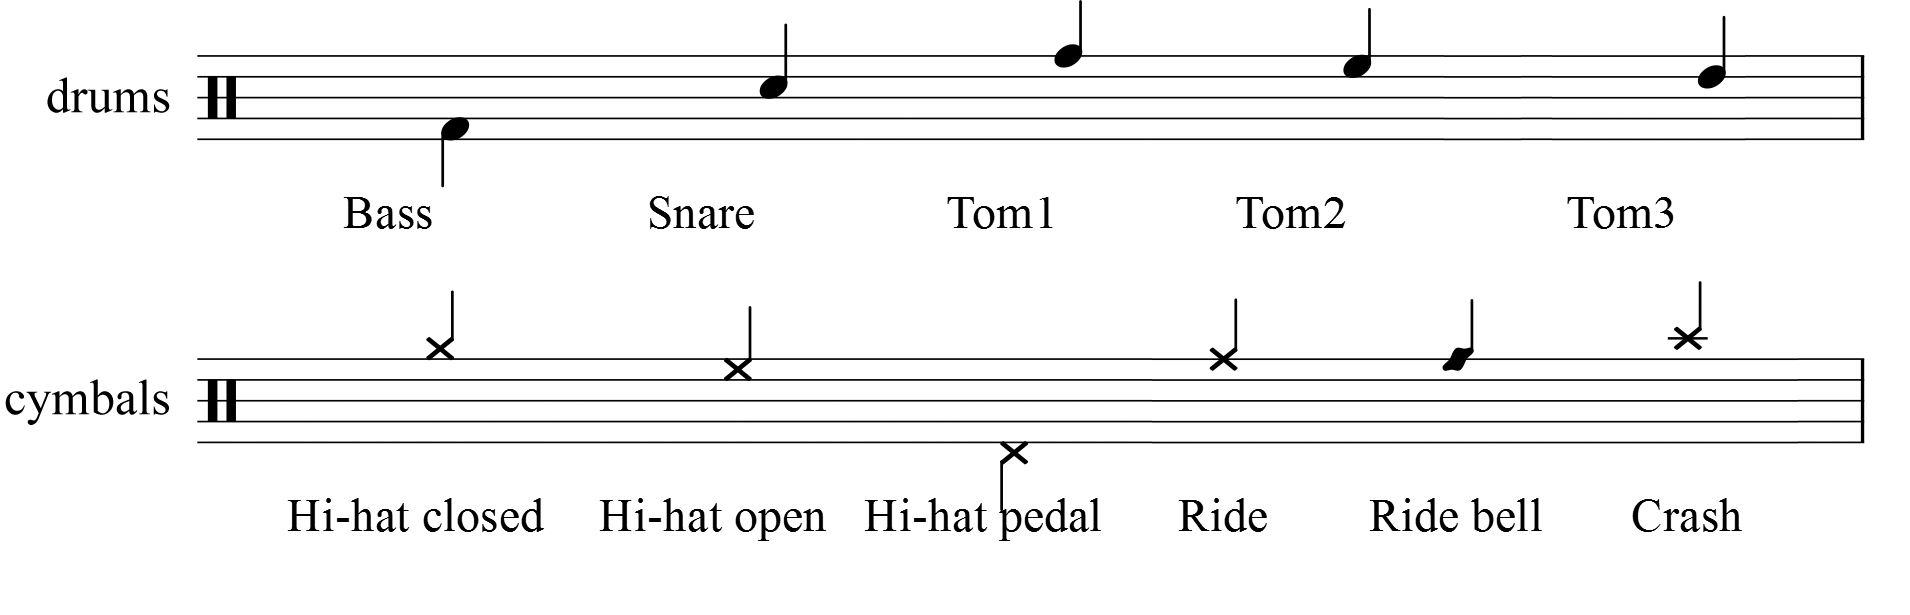
\includegraphics[width=\textwidth]{images/drumsandsheets/notation.png}
	\caption{Drum notation.}
	\label{fig:sheetNotation}
\end{figure}

The notes on the sheet are segmented in small blocks called bars. The bars are separated on the sheet by bar lines.

The number and type of beats in a bar is predefined by the time signature. The time signature is given in the beginning of the sheet after the clef. Example time signatures are $\frac44$, $\frac34$ or $\frac48$. The upper number specifies the number of beats in which the bar is separated and the lower one specifies the note value of a single beat. The note value defines the duration of a note. For this thesis, only the time signature $\frac44$ is used. For this time signature there are counted four beats in one bar, which have the value of a quarter note. 

Important note values in this thesis are the whole note, the halve note, the quarter note, the eighth note and the sixteenth note. The whole note has the length of four quarters and thus has the duration of a whole bar with the time signature $\frac44$. The duration of the recent notes is given proportional to the quarter note. By putting a dot behind a note, the note duration is stretched by the next lower note value. Next to notes, pauses can be displayed. Pauses specify a certain period of time, where no note is played. They can have the same values as notes. Different note and pause values are shown in figure \ref{fig:sheetValues}.

\begin{figure}[h]
	\centering
	
\includegraphics[width=\textwidth]{images/drumsandsheets/note_values.png}
	\caption{Note and pause values.}
	\label{fig:sheetValues}
\end{figure}

In addition to the time signature, the beats per minute (bpm) of a rhythm can be specified . For instance, if a beat is played with 60 bpm, this means one beat per second is played.

More information about the drum notation can be found in \autocite{Stein:2013}.

\subsection{Audio Signal Processing}

Every stroke on a drum or a cymbal creates an analog acoustic signal. This signal is a sinusoidal signal that contains information about the character of the sound it produces. To receive and process this information on a computer, the sounds need to be converted into digital signals. The steps of this process are called sampling and quantization. To provide an insight into the structure of audio signals and the process of quantization, these subjects are introduced in the following. An introduction to signal processing is also given in \autocite{Werner:2012}.

\subsubsection{Audio Signals}

An analog audio signal is a value- and time-continuous, sinusoidal wave. A sample audio signal is shown in figure \ref{fig:audiosignal}. The wave is build by the time $t$ in seconds as x-axis and the amplitude $y(t)$ as y-axis.

% figure audiosignal
\begin{figure}[h]
	\centering
	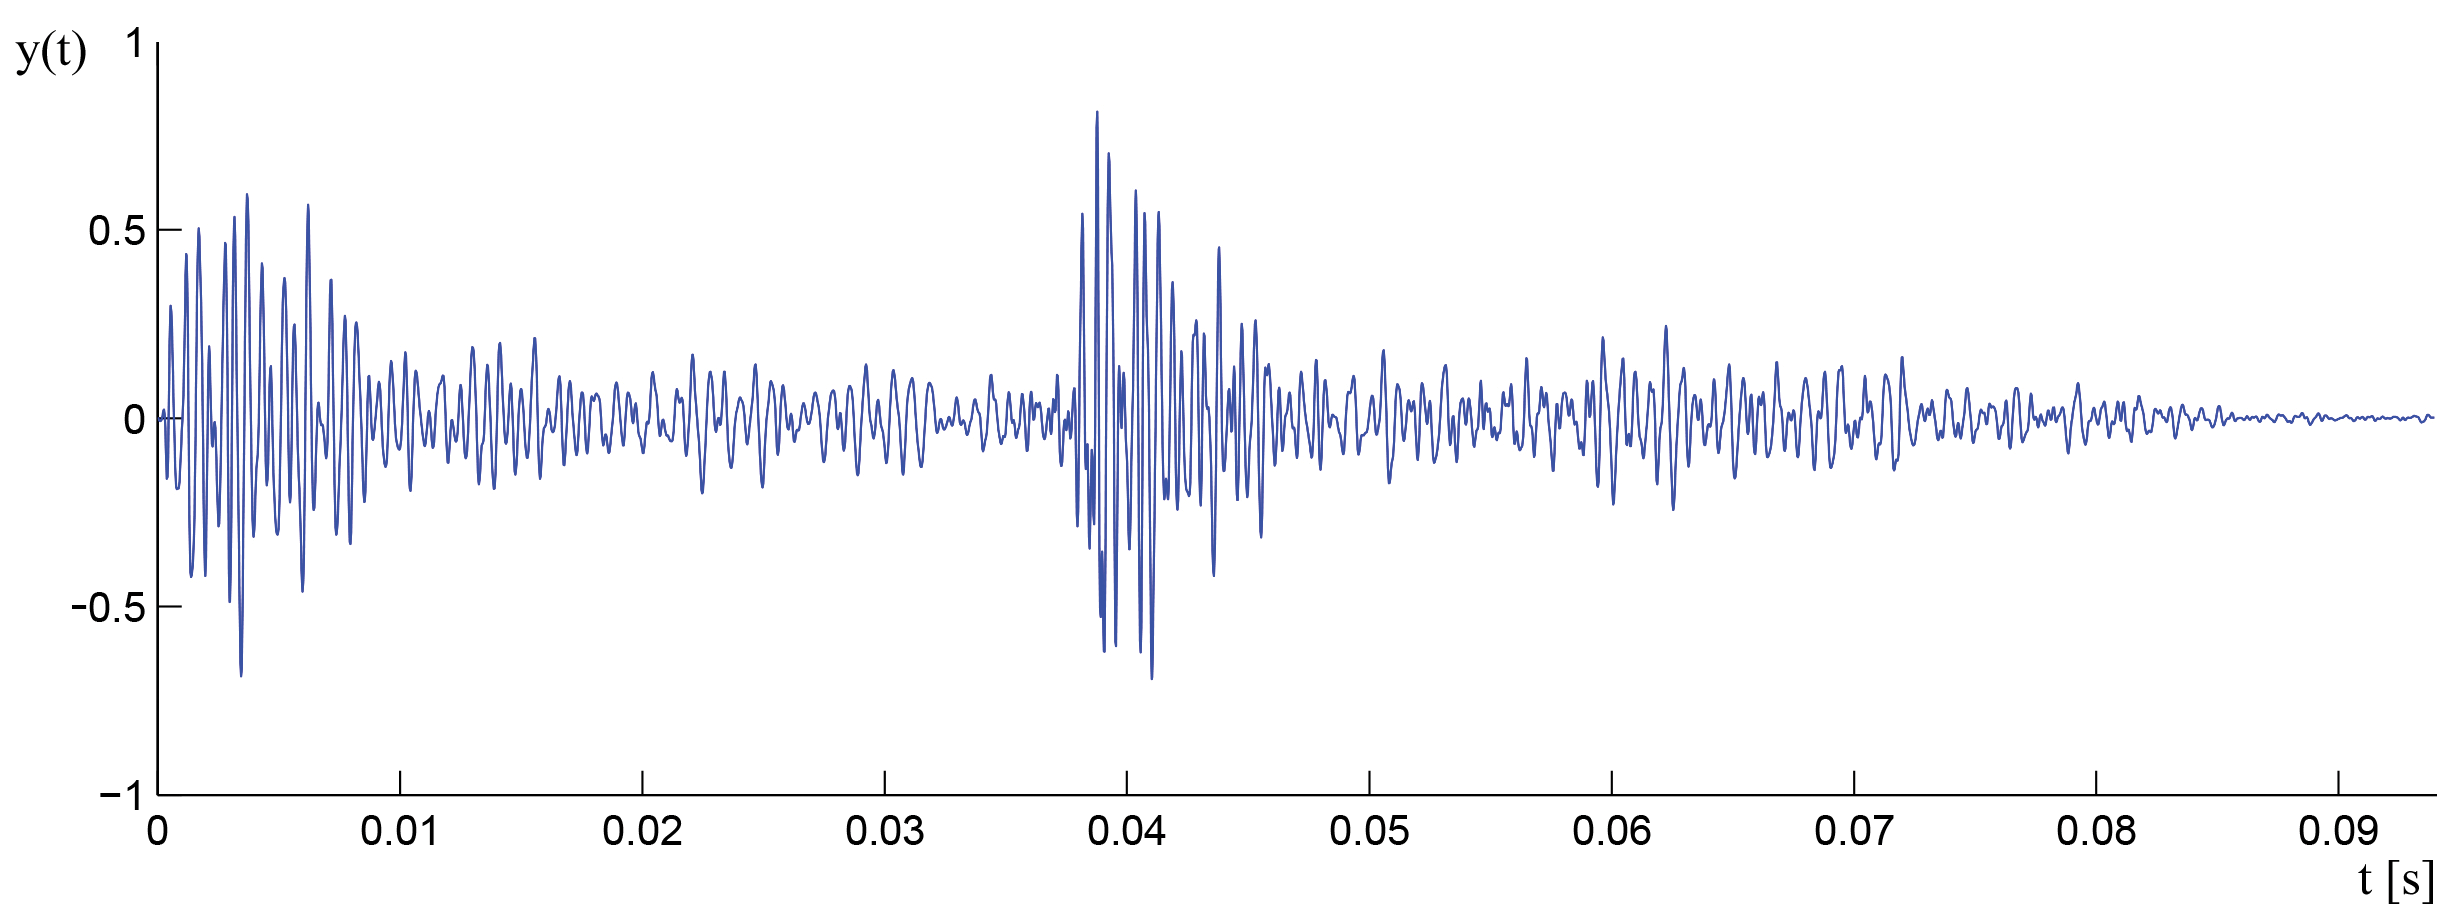
\includegraphics[width=.9\textwidth]{images/audiosignal.png}
	\caption{Example audio signal.}
	\label{fig:audiosignal}
\end{figure}

As introduced in \autocite{Weltner:2013}, the form of a periodic sinusoidal wave is described by its amplitude $A$, its period $\omega$ and its phase $\varphi_0$, as follows:
 
\begin{equation}
	y(t)=A*sin(\omega t+\varphi_0)
\end{equation}

An example sinusoidal wave is shown in figure \ref{fig:sinusoidalexample}. It shows the function
$y(t)=5*sin(2t+\frac{\pi}{2})$.

The amplitude $A$ defines the scaling factor for the sinus function. The maximum value of the function is always the value of this scaling factor. Thus, for $A=5$, the sinusoidal function has the maximum amplitude of $5$ and a minimum amplitude of $-5$.

The period $\omega$ defines the stretching and shrinking factor of the wave. For $\omega =1$, the sinusoidal function has a length of $2\pi$. For all values with $\omega <1$ the wave is stretched and for all values with $\omega >1$ it is shrunken.

The phase $\varphi_0$ defines the shifting of the wave on the x-axis. It is shifted to the left by positive values and to the right by negative values for $\varphi_0$. Considered within the unit circle, $\varphi_0$ describes a temporary shift of the wave by the phase angle $\varphi_0$. Figure \ref{fig:sinewave} shows a sinus function in relation to the phase angle in the unit circle.

%figure 1) function, einheitskreis
\begin{figure}[ht]
	\centering
	\subfloat[Sinus curve in relation to the unit circle.]{
		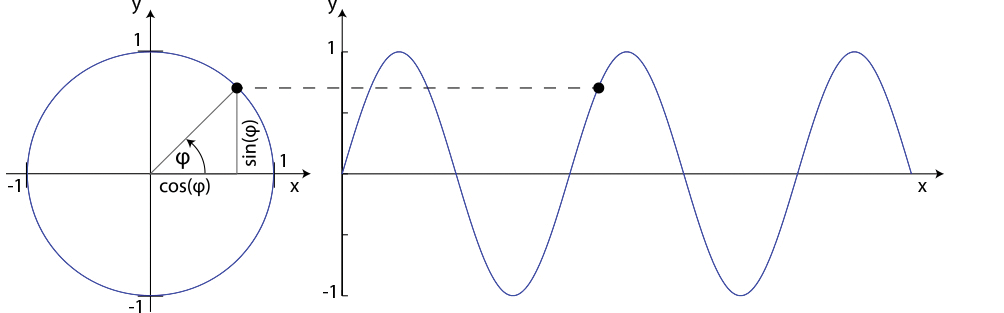
\includegraphics[height=3.0cm]{images/sine1.png}
		\label{fig:sinewave}
	}
	\subfloat[
	Example sinusoidal wave with 
	$y(t)=5*sin(2t+\frac{\pi}{2})$.
	]{
		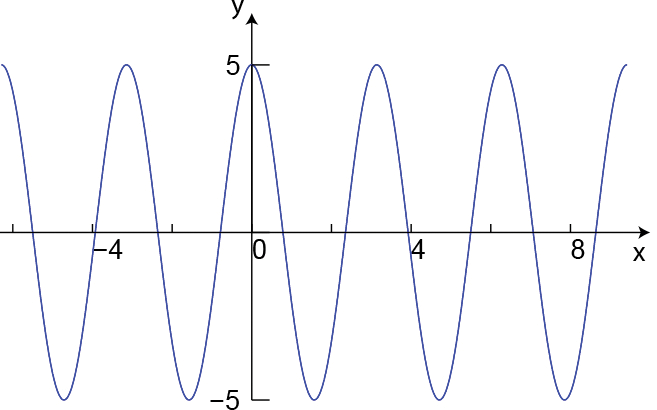
\includegraphics[height=3.0cm]{images/sine2.png}
		\label{fig:sinusoidalexample}
	}
	\caption{
		Sinusoidal functions.
	}
\end{figure}

As shown in figure \ref{fig:audiosignal}, an audio wave generally changes its form over time. Thus, it is an aperiodic signal, which can vary over time in its amplitude $A$, its period $\omega$ and its phase $\varphi_0$.

\subsubsection{Sampling and Quantization}

To process an audio signal on a computer, it needs to be transformed from the analog to a digital (value- and time-discrete) signal. Therefore, sampling and quantization are needed. Figure \ref{fig:quantization} shows a value- and time-continuous signal and a converted value- and time-discrete signal.

% figure analog-digital, quantisierung
\begin{figure}[ht]
	\centering
	\subfloat[Value- and time-continuous signal.]{
		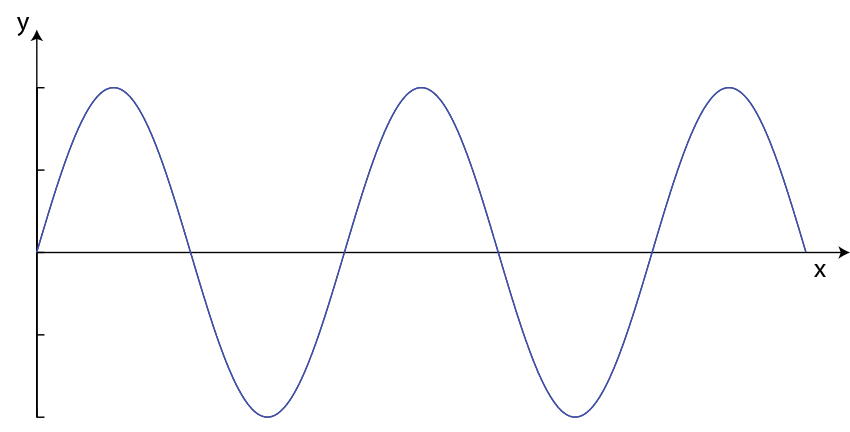
\includegraphics[width=7.2cm]{images/sine3.png}
	}
	\subfloat[Value- and time-discrete signal.]{
		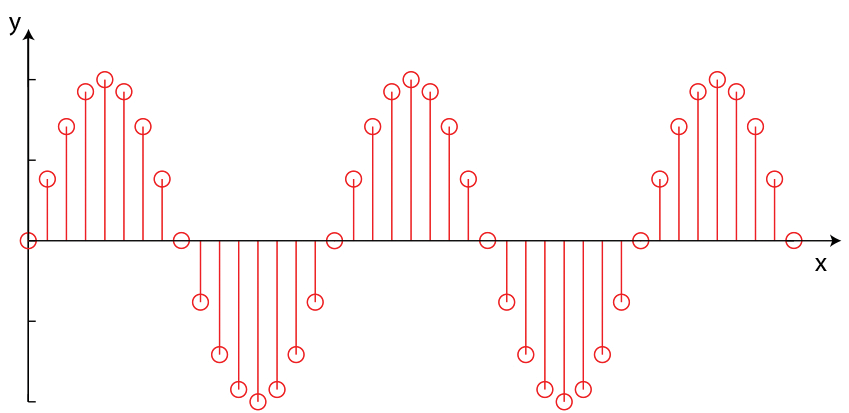
\includegraphics[width=7.2cm]{images/sine4.png}
	}
	\caption{
		Quantization.
	}
	\label{fig:quantization}
\end{figure}

The sampling creates the time discrete signal. Thereby, the sampling rate $f_s$, which is the number of frames per seconds (fps) in the digital signal, is specified in Hz. Typical sampling rates are 8000 Hz, 22.000 Hz or 44.100 Hz. A frame is also called \textit{sample}. To receive a good sampling rate, the sampling theorem, which is described in \autocite{Zoelzer:2008}, needs to be considered. In general, a fast varying signal has to be sampled higher than a slowly varying one. This way, the original signal can be represented with a reasonable degree of accuracy.
%Sampling Theorem Walter seite 56!
% Eine sinnvolle zeitliche Diskretisierung liegt vor, wenn die Veränderungen des analogen Signals durch die Abtastfolge gut wiedergegeben werden. Damit das analoge Signal aus der Abtastfolge durch eine Interpolation hinreichend genau wieder gewonnen werden kann, muss ein sich schnell änderndes Signal häufiger als ein dazu relativ langsam veränderliches Signal abgetastet werden. Diese grundsätzliche Überlegung wird im Abtasttheorem präzisiert.

The quantization displays the signal amplitudes by a given bit rate. By default, a bit rate of 8 bit or 16 bit is used. This procedure is performed by an analog to digital converter. 

Further information about sampling and quantization of analog signals can be found in \autocite{Werner:2012} and \autocite{Zoelzer:2008}.

\subsection{Frequency Spectrum Analysis of Digital Signals} 
For this thesis, the most important signal processing method is the conversion of a digital audio signal to its frequency spectrum. This spectrum displays the distribution of energy within the frequency domain. 

The frequency domain of a digital signal is affected by sampling and sampling rate. If an analog signal is sampled with a sampling rate of 40100 Hz, the frequency range from 0 Hz up to 20050 Hz $($half of the sampling rate$)$ is mirrored between 20000 Hz and 40100 Hz. The amplitudes between 0 Hz and 20050 Hz are the same in both spectra. The effect is shown in figure \ref{fig:analogDigitalSpectra}. 

% The sampling operation leads to a replication of the baseband spectrum of the analog signal [Orf96]. The frequency contents from 0 Hz up to 20 kHz of the analog signal now also appear from 40 kHz up to 60 kHz and the folded version of it from 40 kHz down to 20 kHz. The replication of this first image of the baseband spectrum at 40 kHz will now also appear at integer multiples of the sampling frequency of fs = 40 kHz. But notice that the spectrum of the digital signal from 0 up to 20 kHz shows exactly the same shape as the spectrum of the analog signal. The reconstruction of the analog signal out of the digital signal is achieved by simply lowpass filtering the digital signal, rejecting frequencies higher than f s / 2 = 20 kHz.

% zoelzer figure 1.5
\begin{figure}[h]
	\centering
	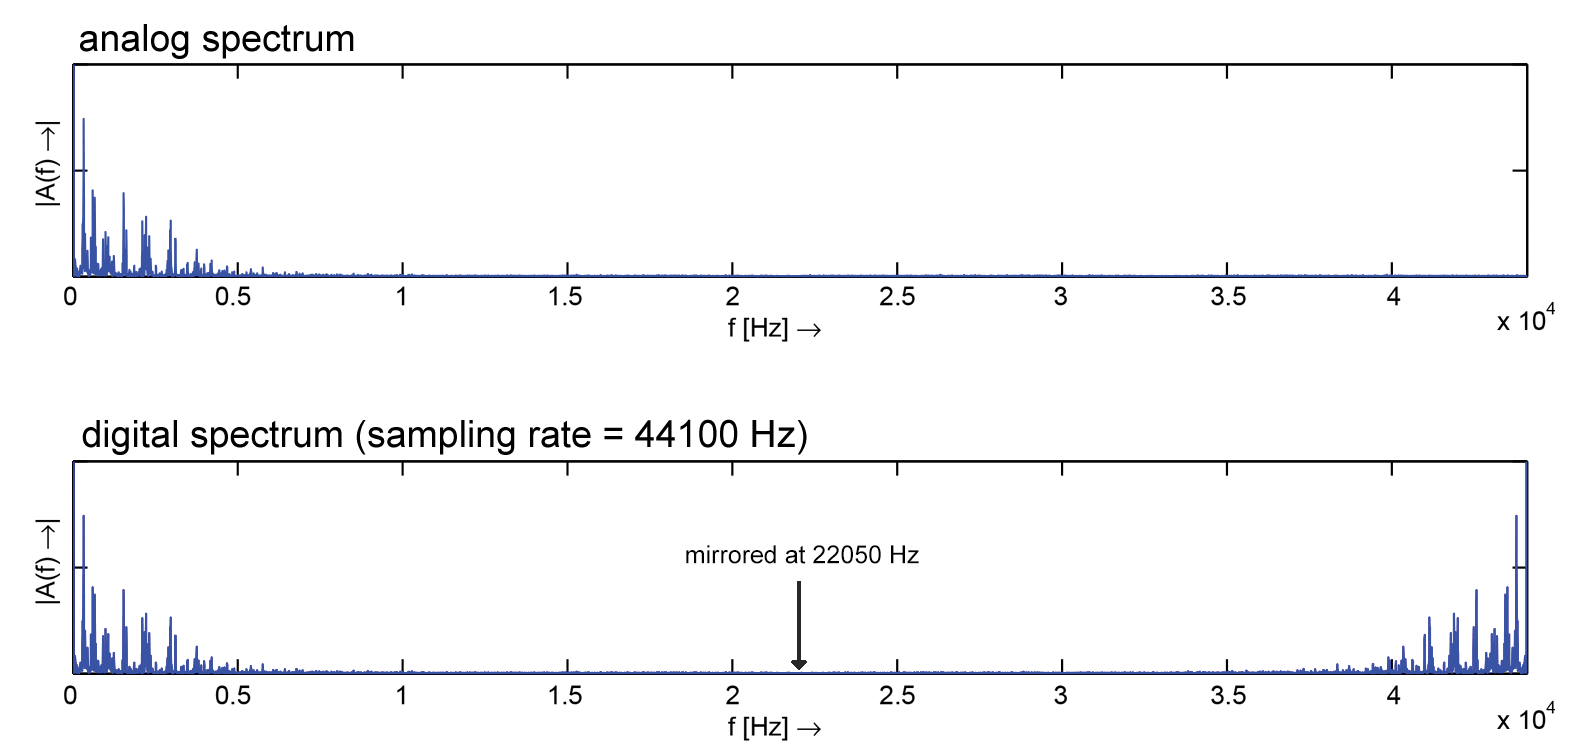
\includegraphics{images/analogDigitalSpectra.png}
	%for reference to this figure
	\caption{ Spectra of analog and digital signals.}
	\label{fig:analogDigitalSpectra}
\end{figure}

\subsubsection{Discrete Fourier Transformation}

To decompose the time series $x[n]$ of an audio signal into its frequency spectrum $X[k]$, the Fourier series and the Fourier transform are fundamental methods. They are based on the research of Jean Baptiste Joseph Fourier in the 18th century. The Fourier series is used to convert periodic time continuous signals and the Fourier transform is used to convert aperiodic time continuous signals. Based on the Fourier series, the \textit{Discrete Fourier Transform (DFT)} can be used on time discrete periodic signals. In contrast to the Fourier transform or Fourier series, the DFT can be used for short time spectral analysis, which is described in section \ref{section:shortTime} \autocite[]{Werner:2012}.


In \autocite[]{Zoelzer:2002} the DFT is defined as a series of DFT-coefficients by

\begin{equation}
X(k)=DFT[x(n)]=\sum_{n=0}^{N-1}x(n)e^{-j2\pi nk/N}, k=0,1,2,...,N-1
\label{equation:DFT}
\end{equation}

\subsubsection{Short Time Spectral Analysis and Windowing} \label{section:shortTime}

A short time spectral analysis is a spectral analysis which is only applied to short blocks of a signal. These blocks are called \textit{windows}. The DFT allows it to be used block oriented because of its periodic exponential function $exp(-j2\pi nk/N)$, which is described in equation \ref{equation:DFT}. It assigns to N elements of a periodic signal exactly N frequency bins in the resulting spectrum. Thus, the larger the window is, the higher the resolution of the resulting frequency spectrum.

In real-time audio processing the incoming signal is divided into a sequence of windows. They can be abutting or overlapping \autocite[]{Werner:2012}.

The DFT assumes that the signal is continued periodically. Hence, for a periodic signal, the window size should be a minimum of an entire period because otherwise there is a loss of information. Further on, as an optimum, the window should begin at the same point in the period as it ends. But this is not possible for audio signals because they are usually not periodic. In this case, not existing spectral components can appear in the frequency domain. This type of occurrences is called \textit{leakage phenomenon} \autocite[]{Werner:2012}.

To reduce the effect of the leakage phenomenon, the form of the window can be changed by applying a so called window function. Thereby, the wave is flattened in its beginning and end. If a window with window function is periodically continued, there is no more leap in the wave. The effect is shown in figure \ref{fig:window1}.

\begin{figure}[h]
	\centering
	\subfloat[Without window function.]{
		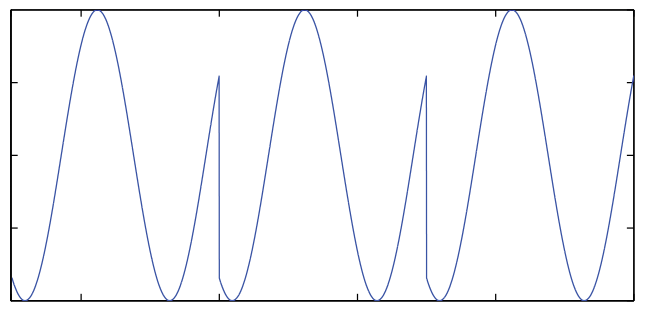
\includegraphics[width=7.2cm]{images/sine5.png}
	}
	\subfloat[With window function (Hamming window).]{
		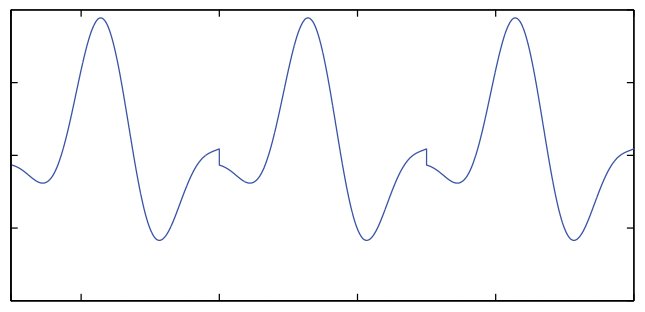
\includegraphics[width=7.2cm]{images/sine6.png}
	}
	%for reference to this figure
	\caption{ Periodically repeated window of values. }
	\label{fig:window1}
\end{figure}

Common window functions in the field of audio processing are the Hamming Window or the Hanning Window. These and other window functions are explained in \autocite[]{Harris:1978}. Figure \ref{fig:window2} shows some common functions.

\begin{figure}[h]
	\centering
	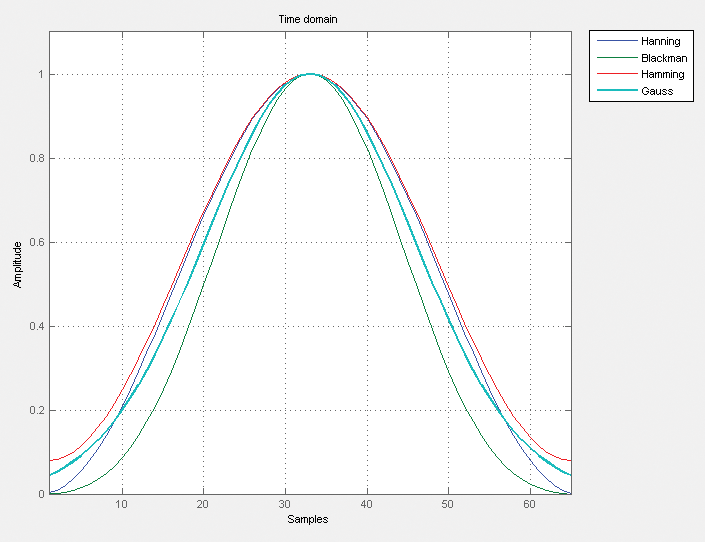
\includegraphics[width=11cm]{images/windowfunctions.png}
	%for reference to this figure
	\caption{Window functions.}
	\label{fig:window2}
\end{figure}

\subsubsection{Fast Fourier Transformation}
The \textit{Fast Fourier Transformation (FFT)} is an efficient version of the DFT. There are many different approaches for FFT algorithms, today. They are based on the fact that a series of real number x[n] with an even length $N=2M$ can be decomposed to a complex series of half the length of N. Thus, the DFT can be decomposed in two parts - one with even and one with odd indices. One of the most popular FFT algorithms is the Radix-2-FFT. The complexity of the direct use of the DFT is $O(N^2)$, whereas the Radix-2-FFT has a complexity of $O(N log_2(N))$. Hence, the FFT allows to use digital signal processing in real-time. 

% Fourier Analysis can be used to identify naturally occurring harmonics (which are, simply put, the basis of all musical composition), to model sound, and to break up sound into the pieces that define it.

% The spectrumo f a digital signal can be computedb y the discrete Fourier transform DFT which is given by
% (1.1)
% The fast version of the above formula is called the fast Fourier transform FFT. The FFT takes N consecutive samples out of the signal z(n) and performs a mathematical operation to yield N sa,mples X ( k ) of the spectrum of the signal. Figure 1.6 demonstrates the results of a, 16-point FFT applied to 16 samples of a cosine signal. The result is normalized by N according to X=abs (fft (x ,N) ) /N; .
% The N samples X ( k ) = X,(k) + j X l ( k ) are complex-valued with a real part XR(IC) and an imaginary parXt ~ ( l cf)ro m which one can compute the absolutvea lue
% (1.2)
% which is the magnitude spectrum, and the phase
% (1.3)
% which is the phase spectrum.

% Frequency Resolution: Zero-padding and Window Functions
% To increase the frequency resolution for spectrum analysis we simply take more samples for the FFT algorithm. Typical numbers for the FFT resolution are N = 256,512,1024,2048,4096 and8 192. If we are only interested in computing thes pectrum of 64 samples and would like to increase the frequency resolution from f,/64 to f,/1024, we have to extend the sequence of 64 audio samples by adding zero samples up to the length 1024 and then performing an 1024-point FFT. This technique is called zero-paddingand is illustrated in Fig. 1.8 and by M-file 1.5. The upper left part shows the original sequence of 8 samples and the upper right part shows the corresponding 8-point FFT result. The lower left part illustrates the adding of 8 zero samples to the original 8 sample sequence up to the length of N = 16. The lower right part illustrates the magnitude spectrum IX(k)l resulting from the 16-point FFT of the zero-padded sequence of length N = 16. Notice the increase in frequency resolution between the 8-point and 16-point FFT. Between each frequency bin of the upper spectrum a new frequency bin in the lower spectrum is calculated. Bins k = 0,2,4,6,8,10,12,14 of the 16-point FFT correspond to bins k = 0,1,2,3,4,5,6,7 of the 8-point FFT. These N frequency bins cover the frequency range from 0 Hz up to v fs Hz.



\subsection{Onset Detection} \label{section:OnsetDetection}

Before a drum stroke can be analyzed it has to be found in the signal stream. For this, onset detection is used. There are many different methods of onset detection right now. \autocite{Bello:2005} describes some important ones. The paper focuses on note onset detection in musical signals.

The audio signal that describes a single note can be divided into several parts. As shown in figure \ref{fig:OnsetDetection1}, \autocite{Bello:2005} differentiates between \textit{onset}, \textit{attack}, \textit{transient} and \textit{decay}. The onset is defined as the point in time, where the wave shows the first signs of a new note. The attack is the interval after an onset, where the amplitude is rising. The transient describes the part of the wave, where the signal evolves. In case of a drum stroke, this would be the time from the first contact of the drum stick on a drumhead until the sound is damped by the stroke. Subsequently, the sound decays. In \autocite{Bello:2005} it is assumed that the human ear cannot distinguish between two transients less than 10 ms apart.

\begin{figure}[h]
	\centering
	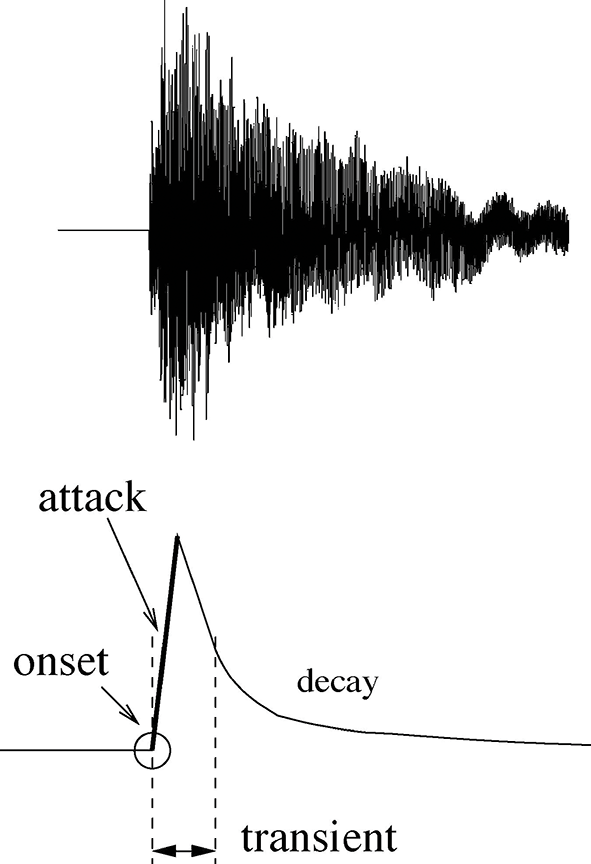
\includegraphics[width=4.0cm]{images/bello_2005_Seite_01_Bild_0001.png}
	\caption{Attack, transient, decay and onset of a sound \autocite[Fig. 1]{Bello:2005}.}
	\label{fig:OnsetDetection1}
\end{figure}

Most onset detection algorithms consist of three steps, like shown in figure \ref{fig:OnsetDetection2}. In the first step, which is optional, the original signal is pre-processed to achieve a better performance in the further steps. Example methods are to separate the signal into multiple frequency bands or to use transient/steady-state separation. The second step is the reduction of the pre-processed audio signal. The reduction is the key process in onset detection. Here, a detection function is created to which a peak picking algorithm can be applied in the last step. These peaks represent the points in time of all onsets in the original audio signal. 

In \autocite[]{Bello:2005} a couple of common onset detection algorithmse are introduced. The paper explains reduction methods based on a signal's amplitude envelope, spectral magnitudes and phases, time-frequency representation and methods based on probabilistic signal models. A basic method that considers the amplitude envelope of audio signals is shown in \autocite[]{Schloss:1985}. It is explained in section \ref{section:OnsetDetectionSchloss}.

\begin{figure}[h]
	\centering
	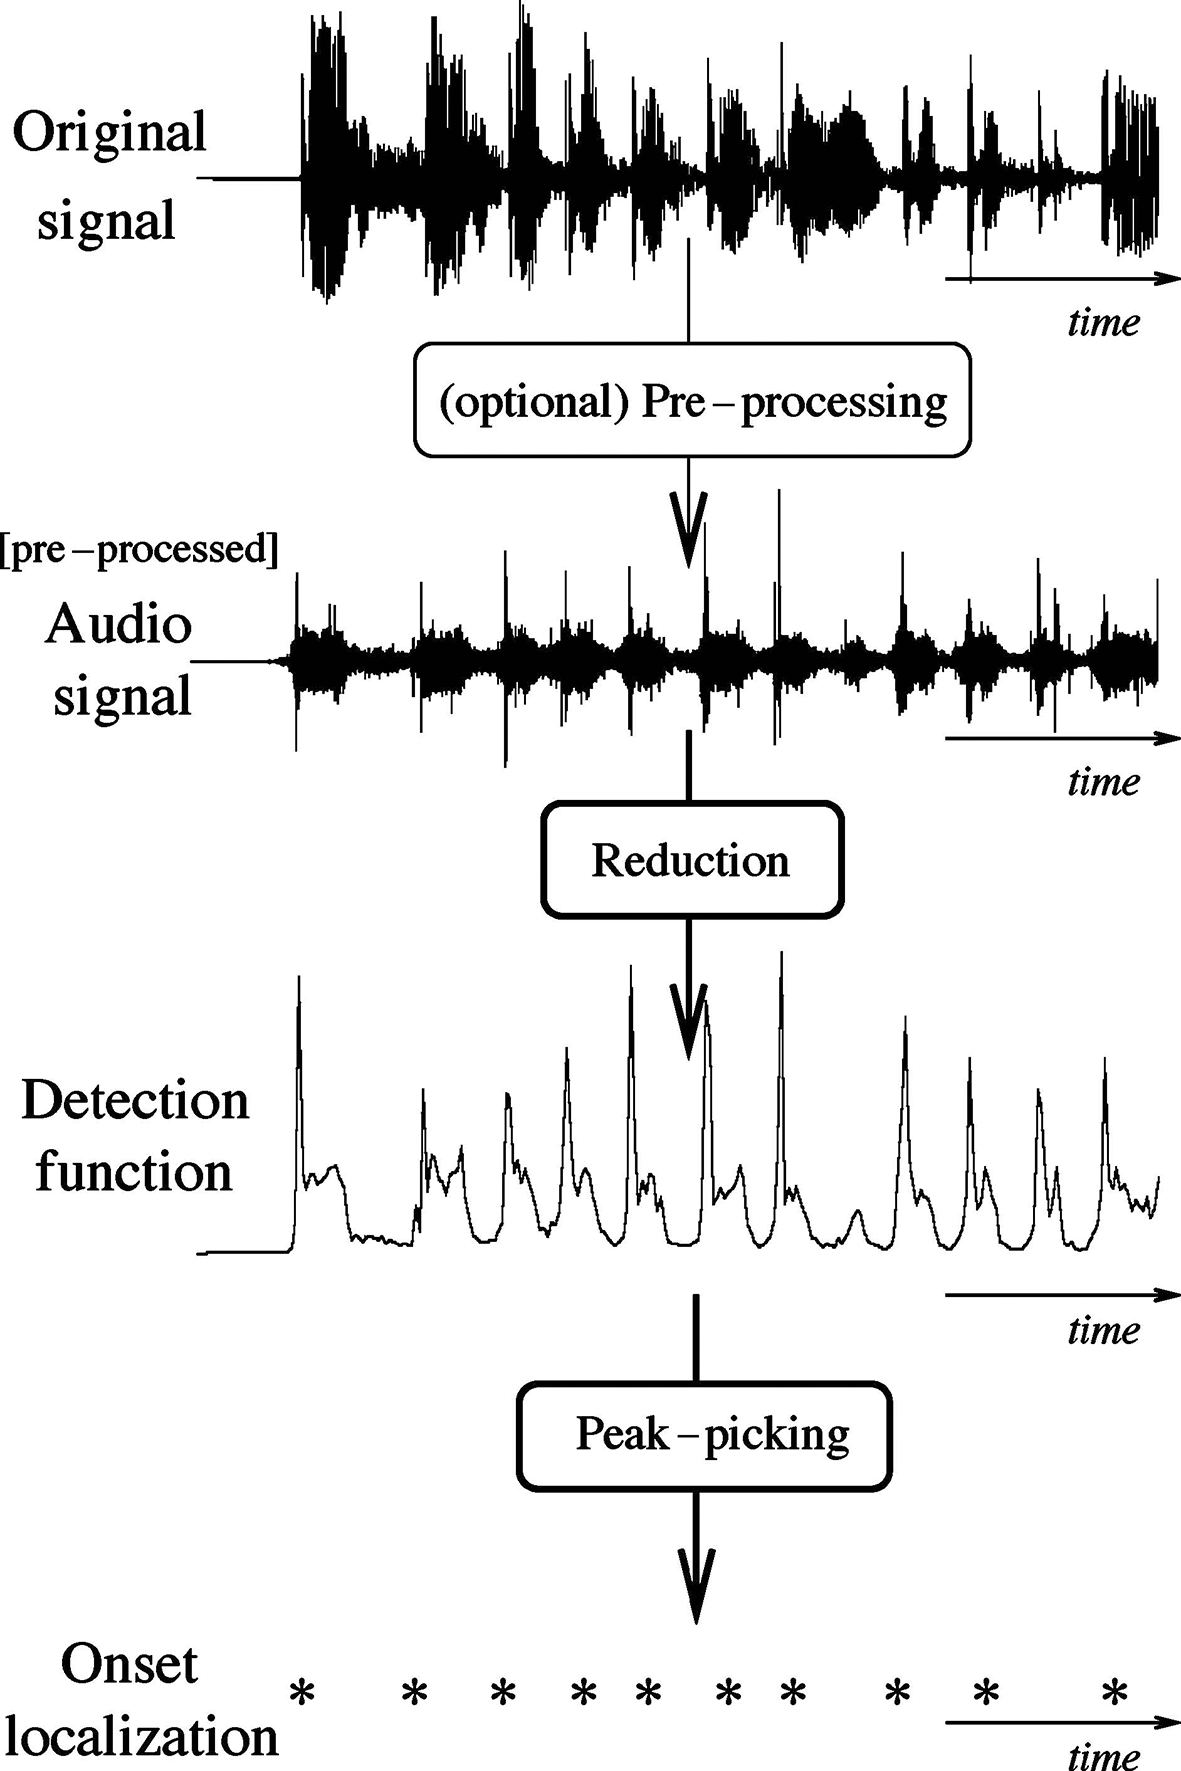
\includegraphics[width=7.0cm]{images/bello_2005_Seite_02_Bild_0001.png}
	\caption{Flowchart of a standard onset detection algorithm \autocite[Fig. 2]{Bello:2005}.}
	\label{fig:OnsetDetection2}
\end{figure}



\subsection{Classification}

After the detection of an onset, the proximate audio information can be classified as one of the drums of the used drum set. Therefore, a classification algorithm is needed. 

Classification describes the attempt to determine class labels for data instances by the use of training data. This process is called \textit{supervised learning}, in contrast to the field of clustering, where \textit{unsupervised learning} is used. A detailed introduction to data classification algorithms and applications can be found in \autocite{Chapman:2015}. There are various different approaches for the classification of data for widespread subjects in computer science.

Generally, a classification algorithm is divided into two steps. The first is the \textit{training} in which a model is built with the help of a training set. The training set contains several labeled data of each possible instance. The second step is the \textit{testing}, where the model is used to assign a label to a test instance. There are also some methods without training. Here, testing refers directly to the training data, which is described as \textit{lazy leaning}. The output of the classification algorithm can be either a discrete label or a numerical score for each possible class.

There are various numbers of classification methods used for different data types. Common data types are text data, multimedia data, uncertain data, time series or discrete sequences. In this thesis audio signals are considers, which is continuous multimedia data. Furthermore, as a main part of the thesis, the frequency spectra of the audio data are used to classify the signals. A frequency spectrum is a sequence, which means a finite, ordered number of values. To classify sequential data, \autocite{Chapman:2015} proposes feature based, distance based and model based classification methods. The general procedure for multimedia data learning is explained by figure \ref{fig:datalearning}. It persists of four steps, which are the preparation of the data, the data pre-processing and feature extraction, the model learning and finally the prediction of unknown data instances.

\begin{figure}[h]
	\centering
	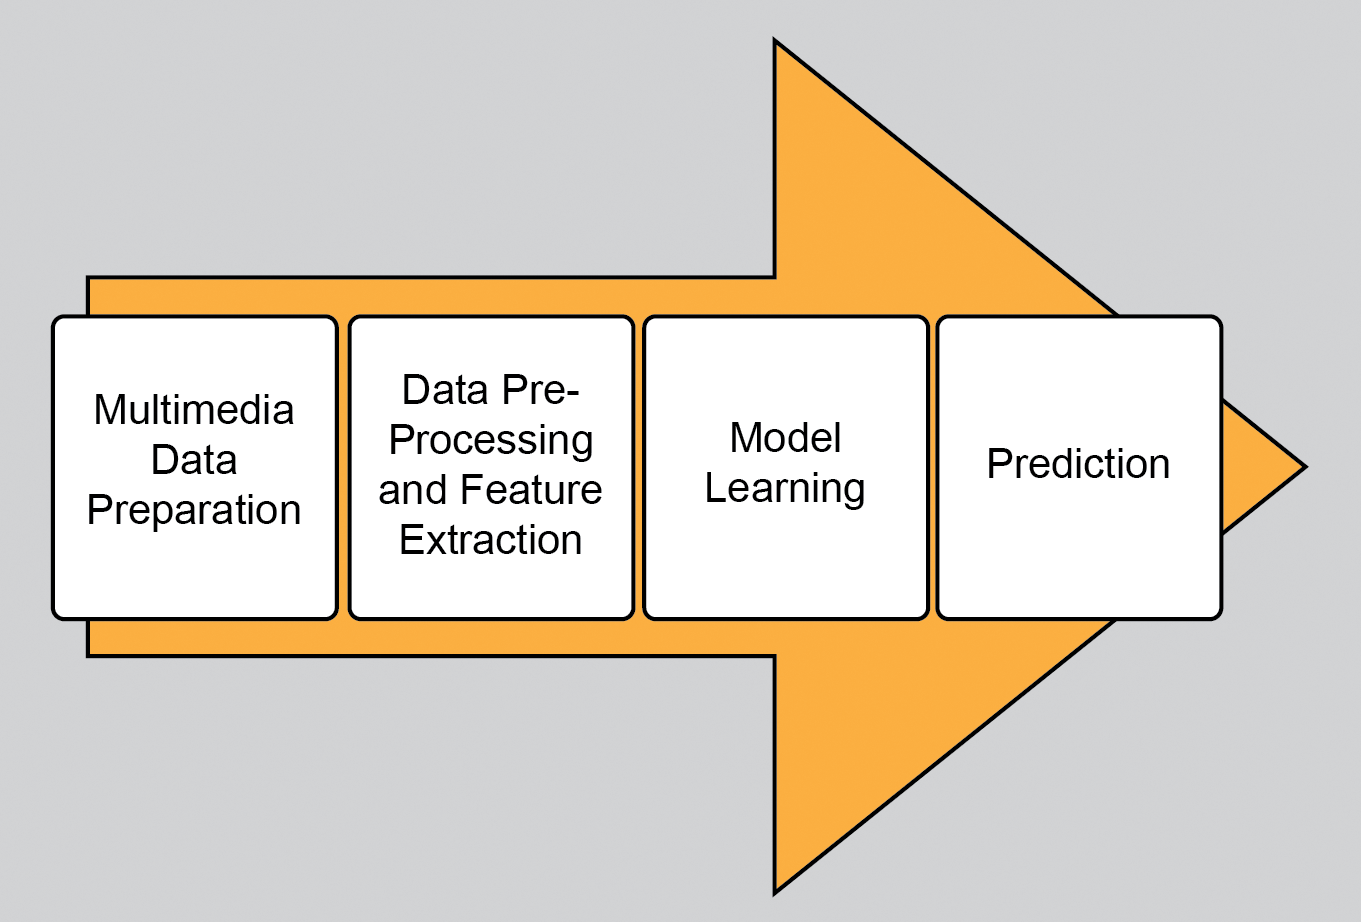
\includegraphics[width=8.0cm]{images/datalearning.png}
	\caption{Flowchart of general multimedia learning process. \autocite[Fig. 12.1]{Chapman:2015}.}
	\label{fig:datalearning}
\end{figure}

\subsubsection{Feature Extraction}

The deciding step in the data classification process is a reasonable data pre-processing and feature extraction. By the extraction of significant features, the model learning and prediction can turn into trivial problems. On the contrary, insignificant features can adulterate the classification result, especially when a small training set is used. As an example, \autocite{Chapman:2015} shows two speech sequences which contain the same sentence spoken by different persons. The resulting waveforms in the time domain are very different and can hardly be assigned as the same sentence. But if the same data is transformed to its frequencies over time, the resulting charts are largely the same. Thus, all used features need to be analyzed in detail.

%\begin{figure}[h]
	%\centering
	%\includegraphics[height=8.0cm]{images/classification/speechexample1.jpg}
	%\caption{Time domain waveform of the same spoken sentence from different persons. \autocite[Fig. 12.2]{chapman:2015}.}
	%\label{fig:speechexample1}
%\end{figure}
%\begin{figure}[h]
	%\centering
	%\includegraphics[height=8.0cm]{images/classification/speechexample2.jpg}
	%\caption{Frequencies over time of the speech in figure \ref{fig:speechexample1} \autocite[Fig. 12.3]{chapman:2015}.}
	%\label{fig:speechexample2}
%\end{figure}

%\subsubsection{Feature Extraction}
%Before the classification is executed, it is important to create a significant feature vector. This vector should only contain values which describe the properties of the classes. Insignificant features can adulterate the classification result, especially when a small training set is used. Using the example of drum sound classification such a feature could be the volume of a drum stroke. If one drum instance has more training data with a higher volume than a second one, all drum with a high volume will be classified as the first drum. Thus all used features has to be analyzed in detail.

For audio data, three different groups of frequently used features can be summarized. These are time domain features, frequency domain features and psycho acoustic features. The latter mainly consider classification of data containing speech and thus irrelevant for this thesis. In time domain, there can be extracted features based on the energy of the audio waveform or the so called zero crossing rate, which counts the number of times the waves goes trough the zero axis within a frame. In the frequency domain an often used feature is the pitch, which defines the fundamental frequency of an audio signal. Subband energy ratios showing the distribution of energy over a predefined frequency band can also be considered. Additionally, there are several methods to extract values based on spectral statistics, like frequency centroids and bandwidth. 

\subsubsection{Feature Based Classification}

The extracted features are usually combined to a feature vector that is used to train a classification model. Thereby, each feature vector represents one of the used class labels. Afterward, new data instances can be predicted with the help of this model. Therefore, the same feature vector needs to be build for the new data. As already mentioned in the preceding section, meaningful features need to be chosen to ensure a high hit-rate for correctly classified instances. Further on, there should not be too many features because the complexity rises with more features for the most classification methods. For feature based classification, common methods are decision trees or statistical methods like naive Bayes, which builds a probabilistic model. In this thesis, decision trees will be used in section \ref{section:method1}. Hence, a short introduction to decision trees is given in the following section.

%Bayesian Classification
%The Bayesian Classification represents a supervised learning method as well as a statistical method for classification. Assumes an underlying probabilistic model and it allows us to capture uncertainty about the model in a principled way by determining probabilities of the outcomes. It can solve diagnostic and predictive problems. 
%This Classification is named after Thomas Bayes ( 1702-1761), who proposed the Bayes Theorem. 
%Bayesian classification provides practical learning algorithms and prior knowledge and observed data can be combined. Bayesian Classification provides a useful perspective for understanding and evaluating many learning algorithms. It calculates explicit probabilities for hypothesis and it is robust to noise in input data.
% decision trees used for this thesis in ... , explained in the following section.

\subsubsection{Decision Trees} 
%introduction to decision trees

One of the most common classification algorithms for solving complex decision-making tasks based on a feature vector is the decision tree. In contrast to other algorithms it's structure is very comprehensible and intuitive for users. An introduction to decision trees is given in \autocite{Chapman:2015}. The decision tree is a rooted, directed tree, which builds a hierarchical structure of conditions. To construct the tree, the extracted feature vectors for every training data instance are passed on to the training algorithm with its appropriate class labels. This training algorithm is called \textit{decision tree induction}. The classical approach for decision tree induction is the top-down selection of partitioning rules on a static data set. It is described in \autocite{Chapman:2015}. After building the tree, it can be used as a classification function to label unseen data instances. 

Every decision tree contains nodes that describe conditions called \textit{splitting rules}. The splitting rules divide the data into separated classes by using the attributes of the feature vector. Most algorithms use one attribute, thus one condition, for each node. The resulting splitting rules are called \textit{univariate}. Some algorithms also use multiple attributes in one node called \textit{multivariate} splitting rules. Furthermore, there are \textit{binary decision trees} and trees with \textit{multiway splits}. In this thesis, binary decision trees are considered. Thus, each node in the tree that is no leaf node has two child nodes.
%Many decision trees are binary, with each partitioning rule dividing its subspace into two parts. Even binary trees can be used to choose among several class labels. Multiway splits are also common, but if the partitioning is into more than a handful of subdivisions, then both the interpretability and the stability of the tree suffers.

To classify an unseen data instance, it passes the nodes by following their splitting rules, beginning at the root node. Thus, each condition in a splitting rule decides to which child node the data instance is going to be transmitted. The process stops when a leaf of the tree is reached. Each leaf node represents a class label.

In most cases, the aim of the decision tree algorithm is not only to find a model that classifies all instances correctly, but also to build a system with a good complexity. The complexity of a decision tree can be measured by the total number of nodes, the total number of leaves, the depth of the tree and the number of attributes used by the splitting rules. To reduce the complexity a method called \textit{pruning} is used, which reduces the depth of the tree \autocite{Bhargava:2013}. This way, the calculation time can be decreased, whereupon the accuracy of the classification may suffer. Thus, a compromise of accuracy and complexity needs to be found.
%{chapman:2015} Ideally, we would like a method with fast tree construction, fast predictions (shallow tree depth), accurate predictions, and robustness with respect to noise, missing values, or concept drift.
%{chapman:2015} The number of possible trees grows exponentially with the number of attributes and with the number of distinct values for each attribute

\begin{table}[htb]
  \caption{Example: Contact Lens Recommendations \autocite{Chapman:2015}}
  \label{tab:c45trainingset} 
	\centering
	\footnotesize
	\begin{tabular}[c]{|c|c|c|c|c|}
	  \hline
		\textbf{Age}	&	\textbf{Near-/Far-sightedness}	&	\textbf{Astigmatic}	&	\textbf{Tears}	&	\textbf{Contacts Recommended} \\
		\hline \hline
		13	&	nearsighted	&	no	&	reduced	&	no \\
		\hline
		18	&	nearsighted	&	no	&	normal	&	yes \\
		\hline
		14	&	nearsighted	&	yes	&	reduced	&	no \\
		\hline
		16	&	nearsighted	&	yes	&	normal	&	yes \\
		\hline
		11	&	farsighted	&	no	&	reduced	&	no \\
		\hline
		18	&	farsighted	&	no	&	normal	&	yes \\
		\hline
		8	&	farsighted	&	yes	&	reduced	&	no \\
		\hline
		8	&	farsighted	&	yes	&	normal	&	yes \\
		\hline
		26	&	nearsighted	&	no	&	reduced	&	no \\
		\hline
		35	&	nearsighted	&	no	&	normal	&	yes \\
		\hline
		39	&	nearsighted	&	yes	&	reduced	&	no \\
		\hline
		23	&	nearsighted	&	yes	&	normal	&	yes \\
		\hline
		23	&	farsighted	&	no	&	reduced	&	no \\
		\hline
		36	&	farsighted	&	no	&	normal	&	yes \\
		\hline
		35	&	farsighted	&	yes	&	reduced	&	no \\
		\hline
		32	&	farsighted	&	yes	&	normal	&	no \\
		\hline
		55	&	nearsighted	&	no	&	reduced	&	no \\
		\hline
		64	&	nearsighted	&	no	&	normal	&	no \\
		\hline
		63	&	nearsighted	&	yes	&	reduced	&	no \\
		\hline
		51	&	nearsighted	&	yes	&	normal	&	yes \\
		\hline
		47	&	farsighted	&	no	&	reduced	&	no \\
		\hline
		44	&	farsighted	&	no	&	normal	&	yes \\
		\hline
		52	&	farsighted	&	yes	&	reduced	&	no \\
		\hline
		46	&	farsighted	&	yes	&	normal	&	no \\
	  \hline
	\end{tabular}
\end{table}

\begin{figure}[htb]
	\centering
	\subfloat[Unpruned tree.]{
		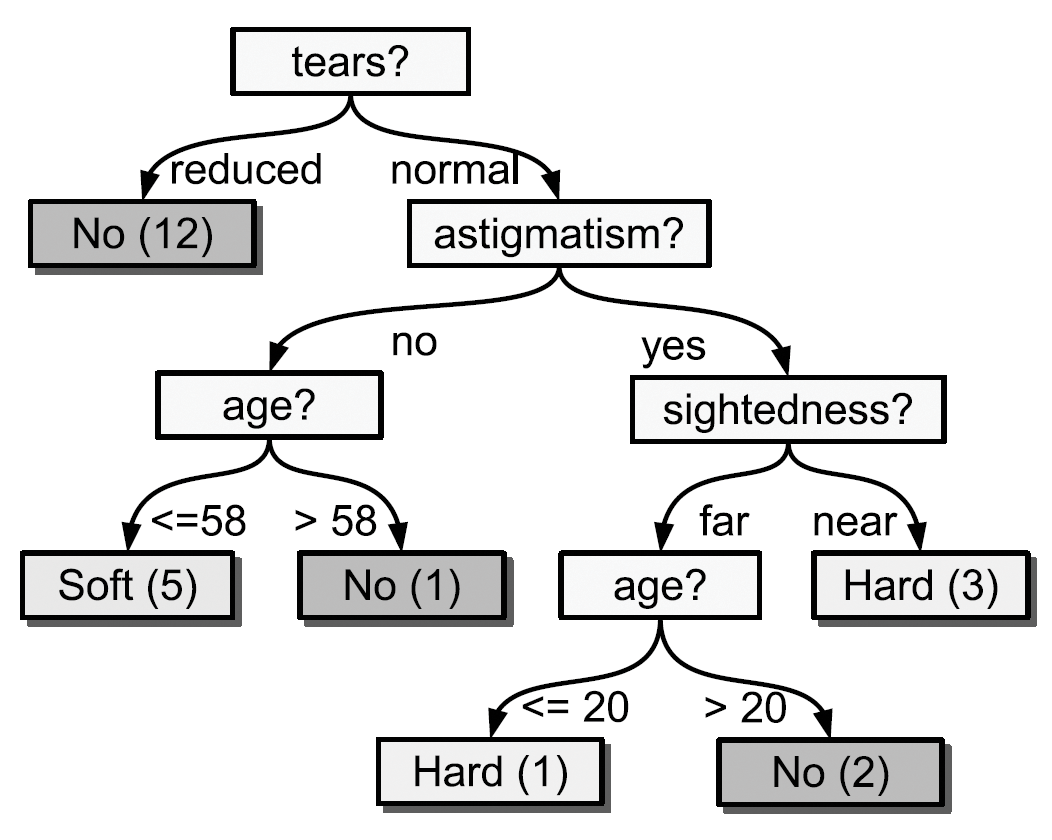
\includegraphics[height=5.0cm]{images/exampletree1.png}
		\label{fig:exampletree1}
	}
	\qquad
	\subfloat[Pruned tree.]{
		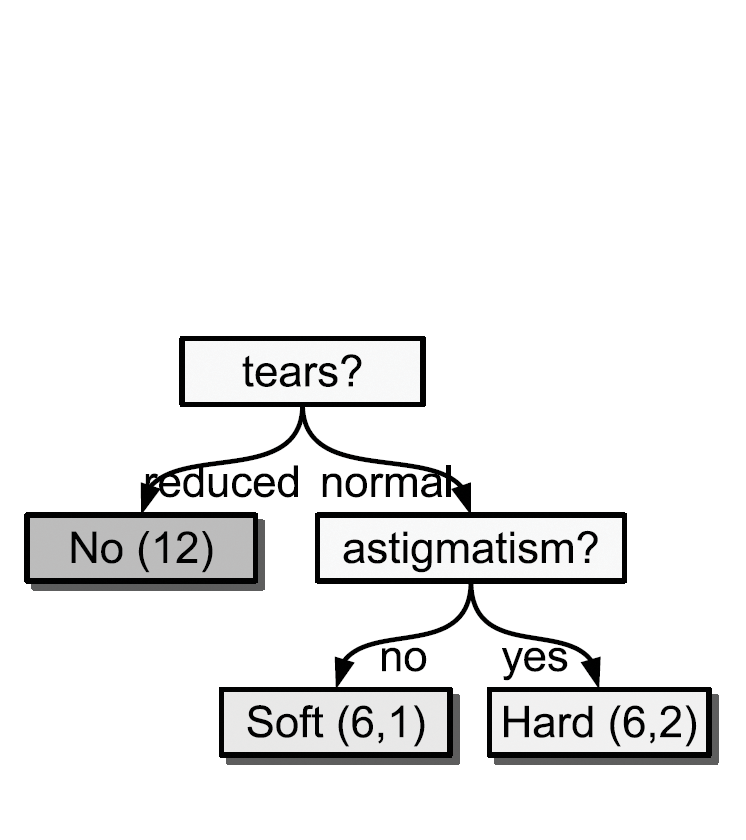
\includegraphics[height=5.0cm]{images/exampletree2.png}
		\label{fig:exampletree2}
	}
	\caption{
		C4.5 decision tree \autocite[Fig. 4.2]{Chapman:2015}
	}
	\label{fig:exampletree}
\end{figure}

For this thesis we will use a C4.5 tree that uses the J48 algorithm. A sample C4.5 decision tree is shown in figure \ref{fig:exampletree}. This tree helps to decide whether a person can wear contact lenses or not. The training set which is used to build the tree is displayed in table \ref{tab:c45trainingset}. Each data record contains information about a person. They include the age of the person as a numerical value and three Boolean values, which are `Near-/Far-sightedness', `Astigmatic' and `Tears'. The last value in the table defines the appropriate class label, which can be `yes' or `no'. The example is taken from \autocite{Chapman:2015}. Figure \ref{fig:exampletree1} shows an unpruned tree that labels all instances correctly. It has a total number of eleven nodes, six leafs and a maximum depth of five. The pruned version of the tree displayed in figure \ref{fig:exampletree2} has only three nodes, two leafs and a depth of two, but labels three instances incorrectly.

\subsubsection{Further Classification Methods}

Next to the feature based methods described in the preceding, there are several other approaches for data classification. In \autocite{Chapman:2015}, distance based and model based methods, which can be used to classify data sequences, are introduced as well.

Distance based classification methods use the distance between two sequences to label unseen data instances. An example for a distance based classification method is the \textit{k-NN (nearest neighbors)} classifier that uses lazy learning. It calculates the distance to all training data to find the nearest neighbor for an unseen data instance. Another common classification system, which uses the similarity instead of the distance between data instances, is the \textit{support vector machine (SVM)}. It calculates the similarity by the construction of a so called \textit{kernel function}. The \textit{SVM} is used in multiple cases to classify audio data.

Model based classification methods build a probabilistic model for each possible class label. These models are used to label unseen data instances. Therefore, a probabilistic function like Bayes rule is used. For each trained class, the probability  is returned that the new data instance is built with the appropriate model. A sample algorithm used to build probabilistic models is the Hidden Markov Model (HMM). It is used by \autocite{Simsekli:2011} for the real-time classification of drum sound, which is described in section \ref{section:realtimeapproach}.

\subsubsection{Evaluation}

To assert the accuracy of a classification algorithm, it needs to be evaluated. Thereby, it has to be regarded that the used test data is not part of the data used to train the system before. Thus, some labeled instances have to be removed before training. There are several methods to do this, such as \textit{hold out} or \textit{cross-validation}. The \textit{hold out} method is the simplest one. Here, a predefined percentage of labeled instances is removed for training and used for testing. In \textit{cross-validation}, the training set is divided into k disjoint subsets. One of the subsets is used for testing, the remaining ones for training. The procedure is repeated k times, so every subset is used for testing, once. This method ensures that every labeled instance is used for training and testing without using trained instances in the test phase.


\subsection{Tools}

To develop and test the algorithms presented in this thesis, MatLab\textsuperscript{\textregistered} and Weka are used as tools.

\subsubsection{MatLab\textsuperscript{\textregistered}}
To extract features of a sound, multiple signal processing methods are necessary. Therefore, MatLab\textsuperscript{\textregistered} \autocite{MathWorks:2014} can be used. MatLab\textsuperscript{\textregistered} is a programming language and interactive environment for numerical computation, visualization, and programming. It provides several built-in function and extension packages for a widespread application range, such as signal processing and communication, image and video processing, control systems, test and measurement, computational finance, and computational biology. For audio processing purposes, it contains a signal processing toolbox that includes several functions, like FFT or window functions. Hence, MatLab\textsuperscript{\textregistered} allows a fast development of new algorithms and can be used to analyze data. In this thesis it is used to develop the onset detection and classification methods and to visualize and evaluate the gained results.

\subsubsection{Weka}

Next to MatLab\textsuperscript{\textregistered}, the data mining tool \textit{Weka} developed by the University of Waikato \autocite{Weka:2014} is used to test and evaluate classification algorithms. Weka contains several machine learning algorithms, such as tools for data pre-processing, classification, regression, clustering, association rules, and visualization. Furthermore, it gives an evaluation overview after each test. A sample output is shown in figure \ref{fig:weka}. Here, a test set with four different drums is used with the Naive Bayes classifier. The labeled data input contains 140 instances and four attributes. It is divided into a training set and a test set with a percentage split of 50 \%. The Weka output gives a detailed overview on the Naive Bayes specific classification results and the time taken to build the model. In the example the time is 0.02 seconds. Further on, the evaluation of the test split is listed. There are 97.15 \% correctly classified and 2.85 \% incorrectly classified instances. The total number of tested instances is 70, whereof 68 instances are correctly classified. Moreover, there is a table showing the detailed accuracy by class and a confusion matrix. The confusion matrix shows as which class the instances are classified. In the example, two instances are classified incorrectly. One with the label `bass' is classified as `tom3' and one with the label `snare' is classified as `tom2'.

\begin{figure}[h]
	\centering
	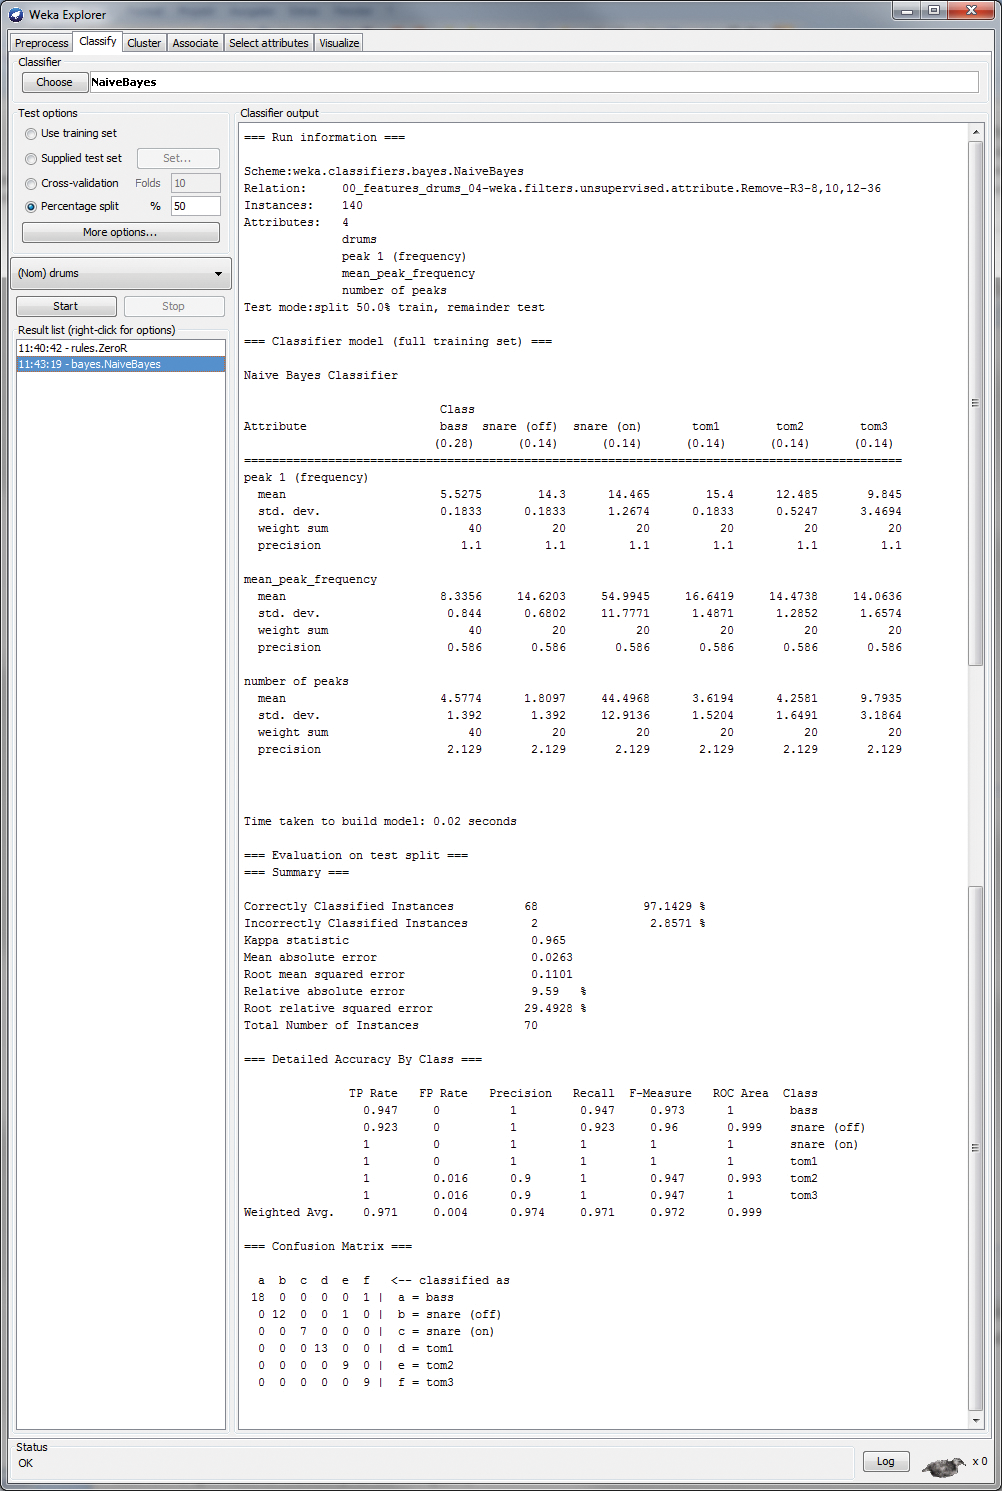
\includegraphics[height=16cm]{images/weka.png}
	\caption{Example Weka output of Naive Bayes classification algorithm for different drum types}
	\label{fig:weka}
\end{figure}


\subsection{Audio Processing in the Web}

As described in section \ref{section:Easydrum}, the aim of this thesis is to develop a listener component for the platform Easydrum, which is able to receive played drum sounds by the audio input through a connected microphone. This listener has to map the incoming sound to the appropriate drums and cymbals and further to save the points in time when a stroke was performed. To realize this, the incoming audio data has to be processed with the help of JavaScript. The data need to be analyzed to find the onsets of performed strokes and to classify these strokes. Hence, a web technology is needed that is able to process audio data.

The actual web standard for the handling of audio data in the web is limited to the \lstinline{<audio>} object of the Audio Data API. These object provides the functionality of playing and get limited information about audio data, but does not enable editing or creation of data. Other limited technologies used to access audio information in recent web applications are Flash or the QuickTime plug-in. However, Easydrum tries to use modern web technologies and thus wants to operate without Flash and QuickTime. As described in section \ref{section:Easydrum}, it uses the Web Midi Api \autocite{WebMidiApi:2015} to receive MIDI input in the browser. This API is not yet a standard but is already largely accessible with the Google Chrome browser and can be simulated in other browsers with the help of the JazzPlugin \autocite{JazzPlugin:2015}.

Concurrently with the Web Midi API, the W3C has been developing the Web Audio API, which is specified by the Audio Working Group as an Editor's Draft \autocite{WebAudioApi:2015}. It is a high-level JavaScript API for processing and synthesizing audio data in web applications. It offers the possibility to create interactive applications with audio content just as audio recorder, sequencers or games with audio content. It can receive audio data from input devices, process them and send them to output devices. This procedure is realized via the provided audio context, which contains different audio processing modules. To process audio operations, audio nodes are used inside the audio context. Different audio nodes can be linked together by their inputs and outputs to form an audio routing graph. According to \autocite{WebMidiApiMDN:2015}, the timing of the Web Audio API `is controlled with high precision and low latency, allowing developers to write code that responds accurately to events and is able to target specific samples, even at a high sample rate.' Additionally, it can be used with the canvas 2D of HTML 5, which is used by Easydrum. Like the Web Midi API, the functionality of the Web Audio API is already largely accessible in the Google Chrome browser. The main methods of the API are also implemented in Firefox since version 25. For browsers that don't support the Web Audio API, there are different JavaScript libraries that provide different fallback solutions to the Audio Data API or to Flash. An example for a library is WAAPISim \autocite{WAAPISim:2015}.

Next to processing audio data, it is required for the Easydrum extension to get access to a microphones input data. This functionality is provided by the WebRTC, which has been developed for the real-time communication between browsers. It is able to receive video and audio streams from local devices like web cams and microphones. The received audio stream can be processed by the Web Audio Api. The WebRTC version 1.0 was published as a working draft \autocite{WebRTC:2015}. 

Hence, the Web Audio API combined with the WebRTC provides the required functionality for the Easydrum extension developed in this thesis.

%An AudioBuffer takes as its parameters a number of channels (1 for mono, 2 for stereo, etc), a length, meaning the number of sample frames inside the buffer, and a sample rate, which is the number of sample frames played per second.
%A sample is a single float32 value that represents the value of the audio stream at each specific point in time, in a specific channel (left or right, if in the case of stereo). A frame, or sample frame is the set of all values for all channels that will play at a specific point in time: all the samples of all the channels that play at the same time (two for a stereo sound, six for 5.1, etc.)
%When a buffer plays, you will hear the left most sample frame, and then the one right next to it, etc, etc. In the case of stereo, you will hear both channels at the same time. Sample frames are very useful, because they are independent of the number of channels, and represent time, in a useful way for doing precise audio manipulation.
%var context = new AudioContext();
%var buffer = context.createBuffer(1, 22050, 22050);
%If you use this call, you will get a mono buffer (one channel), that, when played back on an AudioContext running at 44100Hz, will be automatically *resampled* to 44100Hz (and Therefore yield 44100 frames), and last for 1.0 second: 44100 frames / 44100Hz = 1 second.

%In general, audio visualizations are achieved by accessing an ouput of audio data over time (usually gain or frequency data), and then using a graphical technology to turn that into a visual output (such as a graph.) The Web Audio API has an AnalyserNode available that doesn't alter the audio signal passing through it, but instead outputs audio data that can be passed to a visualization technology such as <canvas>.

%The Web Audio API uses a planar buffer format: the left and right channels are stored like this:
%LLLLLLLLLLLLLLLLRRRRRRRRRRRRRRRR (for a buffer of 16 frames)
%The alternative is to use an interleaved buffer format:
%LRLRLRLRLRLRLRLRLRLRLRLRLRLRLRLR (for a buffer of 16 frames)
%This format is very common for storing and playing back audio without much processing, for example a decoded MP3 stream.
%The Web Audio API exposes *only* planar buffers, because it's made for processing. It works with planar, but converts the audio to interleaved when it is sent to the
%sound card, for playback. Conversely, when an MP3 is decoded, it starts off in interleaved format, but is converted to planar for processing.




\newpage
\section{Related Work}
\label{section:relatedWork}
% Darstellung des aktuellen Wissens zum Thema (Literaturphase – Grundlagen)
% Hier ist ein Überblick über das Fachthema und die Begrifflichkeiten sowie eine Darstellung bestehender Lösungsansätze/Technologien anhand von Quellen aus der wissenschaftlich-technischen Literatur zu erarbeiten. Besonderes Augenmerk ist auf die korrekte Zitierweise von Quellen zu legen. Anderen LeserInnen der Arbeit soll damit das Verständnis für die darauf folgenden Teile der Arbeit erschlossen werden. Inhalte flüchtiger Quellen (Websites) sind geeignet, müssen aber gesichert werden (CD/DVD)


There are a couple of works relating to the subject of this thesis. Thus, in this chapter some relevant work about onset detection (section \ref{section:OnsetDetectionSchloss}), classification (section \ref{section:ClassificationChristophersen}) and the real-time analysis of percussive sound (section \ref{section:realtimeapproach}) are considered.

\subsection{Onset Detection} \label{section:OnsetDetectionSchloss}

There are many different approaches to onset detection algorithms, today. Recent onset detection generally consists of complex algorithms using calculations within the frequency domain. An example is `the use of phase and energy for musical onset detection in the complex domain', described in the paper of \autocite{Bello:2005}. Such algorithms are focused on note onset detection. 

In contrast to the onset of a drum stroke, the onset of a note does not necessarily cause a rise of the amplitude in the time domain. So note onset detection is much more complicated than the detection of drum strokes considered in this thesis. Note onset detection is much more complicated than the detection of drum strokes considered in this thesis. In contrast to the onset of a note, the onset of a drum stroke always causes a rise of the amplitude in the time domain. Hence, for the onset detection of drum strokes, it is sufficient to analyze the amplitude gradient in the time domain. A more complex algorithm would possibly produce better results, but it would also have a longer runtime. This would be a disadvantage because the algorithm that is developed in this thesis shall be able to run in real-time. An appropriate runtime avoids a delay while the software is running.

Besides the runtime, another aspect needs to be considered to enable the algorithm to run in real-time. A standard onset detection algorithm as described in section \ref{section:OnsetDetection} can't be used because it pre-processes and analyzes the entire sound file before the onsets can be detected. In case of a real-time algorithm, only the actual frame of an incoming audio stream can be considered, and all frames before the actual one. Hence, an algorithm that separates the signals in several frames and analyzes them consecutively is needed. This requirement is fulfilled with the onset detection algorithm in the dissertation of \autocite{Schloss:1985}, which deals with the automatic transcription of percussive music. At this early stage of computer science the computing power was much lower than today, so it can be assumed that the algorithm runs very fast on present machines. 

The algorithm of W. Andrew Schloss detects onsets by detecting abrupt increases of energy in the time domain of an audio signal. In a first step, an amplitude envelope is created. Therefore, the signal is divided into small windows. For each window, the maximum and minimum peak are found. By connecting all maximum peaks and all minimum peaks, the envelope is built. On this envelope, a so-called slope detector is applied. It calculates a linear regression over several points of the amplitude envelope. In the following step, attacks are searched in the resulting slope array. The first attack is detected by searching the slope array for a sudden increase during a given duration. Further attacks are found by analyzing local maxima and minima. If a local maximum is found the following data points are analyzed for a given time period to assert if the inequality persists. After each detected attack, there is a lock for a defined time interval, where no more attacks may be detected.

\subsection{Classification} \label{section:ClassificationChristophersen}

An approach for classification of drum types that are similar to the subject of this thesis, is documented in \autocite{Christophersen:2007} by students of the Aalborg University. The main difference is that the algorithm developed in this paper does not run in real-time. Furthermore, only three different drum types are considered, which are a bass drum, a snare drum and a hi-hat. 

The system described in \autocite{Christophersen:2007} consists of four components. In a first step, a sound file sampled with a sampling rate of 44.1 kHz and a resolution of 16 bit, is analyzed by an onset detector to find all onsets. The onset detector divides the sound file into several sound clips, each including one drum stroke. Subsequently, each sound clip is analyzed by a feature extractor. In the last step, the extracted features are used in a feature vector for classification.

%\begin{figure}[h]
	%\centering
	%\includegraphics{images/christopherson.jpg}
	%%for reference to this figure
	%\caption{ Drum recognition system in \autocite{Christophersen:2007} by the Aalborg University.}
	%\label{fig:christopherson}
%\end{figure}

The paper considers different types of features. These are features based on the time domain, features based on the frequency spectrum and features based on cross correlation with templates in time domain.

Two time domain features are extracted with the help of a modified version of the ADSR model, which envelopes the amplitude. ADSR stands for attack time, decay time, sustain level and release time. The model is examined in detail in \autocite{Campbell:2001}. According to \autocite{Christophersen:2007}, only the attack time and the decay time are significant for drums and therefore used as features. Furthermore, a so called \textit{crest factor} is used for the feature vector. It describes the relation between the peak value and RMS-energy of a sound clip.

Frequency domain features are based on parametric and non-parametric methods. 

The non-parametric frequency analysis uses the FFT implemented in MatLab\textsuperscript{\textregistered}. Here, the power of several subbands and the FFT-Spectral centroids are extracted for each drum and used as features. The subbands are manually chosen by examining the spectrum of each used drum type. They range from 50Hz to 170 Hz, from 170 Hz to 260 Hz, from 260 Hz to 4 kHz and from 4 kHz to 10 kHz. Further on, eight octave divided bands from 50 Hz to 12.8 kHz are calculated. To calculate the spectral centroids the paper uses equation \ref{equation:SC}. In the equation, SC defines the spectral centroid, k defines the lower limit and N the upper limit of the frequency band, f(n) is the frequency component of n and x(n) the amplitude of f(n).

\begin{equation}
	SC = \frac{\sum_{n=k}^{N-1}f(n)x(n)}{\sum_{n=k}^{N-1}x(n)}
	\label{equation:SC}
\end{equation}

The parametric frequency analysis is done with the help of the LPC analysis, which is explained in detail in \autocite{Christophersen:2007}. It tries to display a model that fits to the input signal. Extracted features are peak frequencies, spectral centroids and subband power. Furthermore, the DC-component is used. It is described as an error of the modeling of an input signal. The used feature represents the relation between the DC-amplitudes and low frequency content.

For the template-based features, generated templates for time and frequency domain are compared with the sound clips. To construct the templates, the mean of the Fourier transformed and normalized clips is calculated. For the time domain template the inverse Fourier Transform is assigned subsequently. The template comparison is done by cross-correlating the templates with the Fourier transformed clip.

Finally, the two most significant features (LPC-DC and FFT-Spectral Centroid) are chosen and sent to a two-dimensional Bayesian classifier. Thus, all tested clips are classified correctly.

\subsection{Real-Time Approach} \label{section:realtimeapproach}

An approach to develop a system that runs in real-time is introduced in \autocite{Simsekli:2011}. The article was published on the European Signal Processing Conference in 2011. It presents a real-time recognition of percussive sounds by a probabilistic model-based method. Thereby, it focuses on low-latency, classification accuracy and reliability. The system shall be usable for interactive systems. As a sample application, the paper proposes a rhythmic tutoring system that is similar to Easydrum. The system reacts to the user input after giving instructions to learn percussive rhythms.

In contrast to the preceding approaches, the paper of \autocite{Simsekli:2011} does not divide the onset detection and the classification into two steps, but combines them in one detection algorithm. This algorithm is able to receive events during its run time and to classify them in real-time. It is based on the probabilistic template-based models described in \autocite{Simsekli:2010}, which are used for online pitch tracking. A probabilistic generative model is built that assigns event labels for each trained sound. Thereby, the audio signal is divided into subsequent time frames. Each frame is transformed to its frequency domain with the help of the discrete Fourier transform. If there is an event in a time frame, a class label is assigned to it. Sample events are hand claps or the hit, sustain and release of a percussion. Thus, in contrast to the approach in this thesis, not only the attack of a stroke is detected. To assign an incoming sound to a class label, a Hidden Markov Model is used. Further on, post processing is used to avoid multiple detections of the same stroke by defining a period of time after a detected event where no further event may be detected.

The system is based on supervised learning, so it is trained with all possible stroke types. Different kinds of hand claps and turkish percussive instruments are tested. For the percussion instruments, two different membraphones (Darbuka and Bendir) are trained, each with two different stroke types (`düm' and `tek'). For each stroke type, there are 40 instances recorded. The training of the introduced method is performed offline. It includes the creation of templates for each trained sound. The class labels are added manually. 

The by \autocite{Simsekli:2011} developed algorithm is tested with simple rhythmic patterns containing one stroke at a time. It is reached an overall accuracy for the system running in real-time of 61 \%.
%  no simultaneous sounds

 





\newpage
\section{Methods} \label{section:methods}
% Diskussion möglicher Methoden und Lösungswege (Machbarkeitsphase – Analyse)
% Zu Beginn dieses Teils erfolgt eine Gegenüberstellung prinzipiell möglicher Methoden der wissenschaftlichen Herangehensweise an die Themenstellung sowie eine Abschätzung und Diskussion der Erfolgsaussichten der gewählten Methode. Daraufhin sollen anhand von konkreten Varianten verschiedene Lösungsansätze für das Thema erläutert werden, und zwar im Licht der Ergebnisse der Literaturphase einerseits, und in Hinblick auf innovative Lösungen für das Anwendungsfeld (Unternehmen bzw. Institution) andererseits.

In this chapter, the required methods for the aimed extension to the platform Easydrum are developed. 

The extension shall receive an audio stream recorded by a microphone on a browser. It shall detect and classify all drum strokes contained in this audio stream. The point in time of a stroke and the played component of the drum set shall be transmitted to the existing Easydrum platform.

The aimed system shall consist of two components as displayed in figure \ref{fig:architecture}. These are a training system and a real-time drum sound analyzer. 

\begin{figure}[ht]
	\centering
	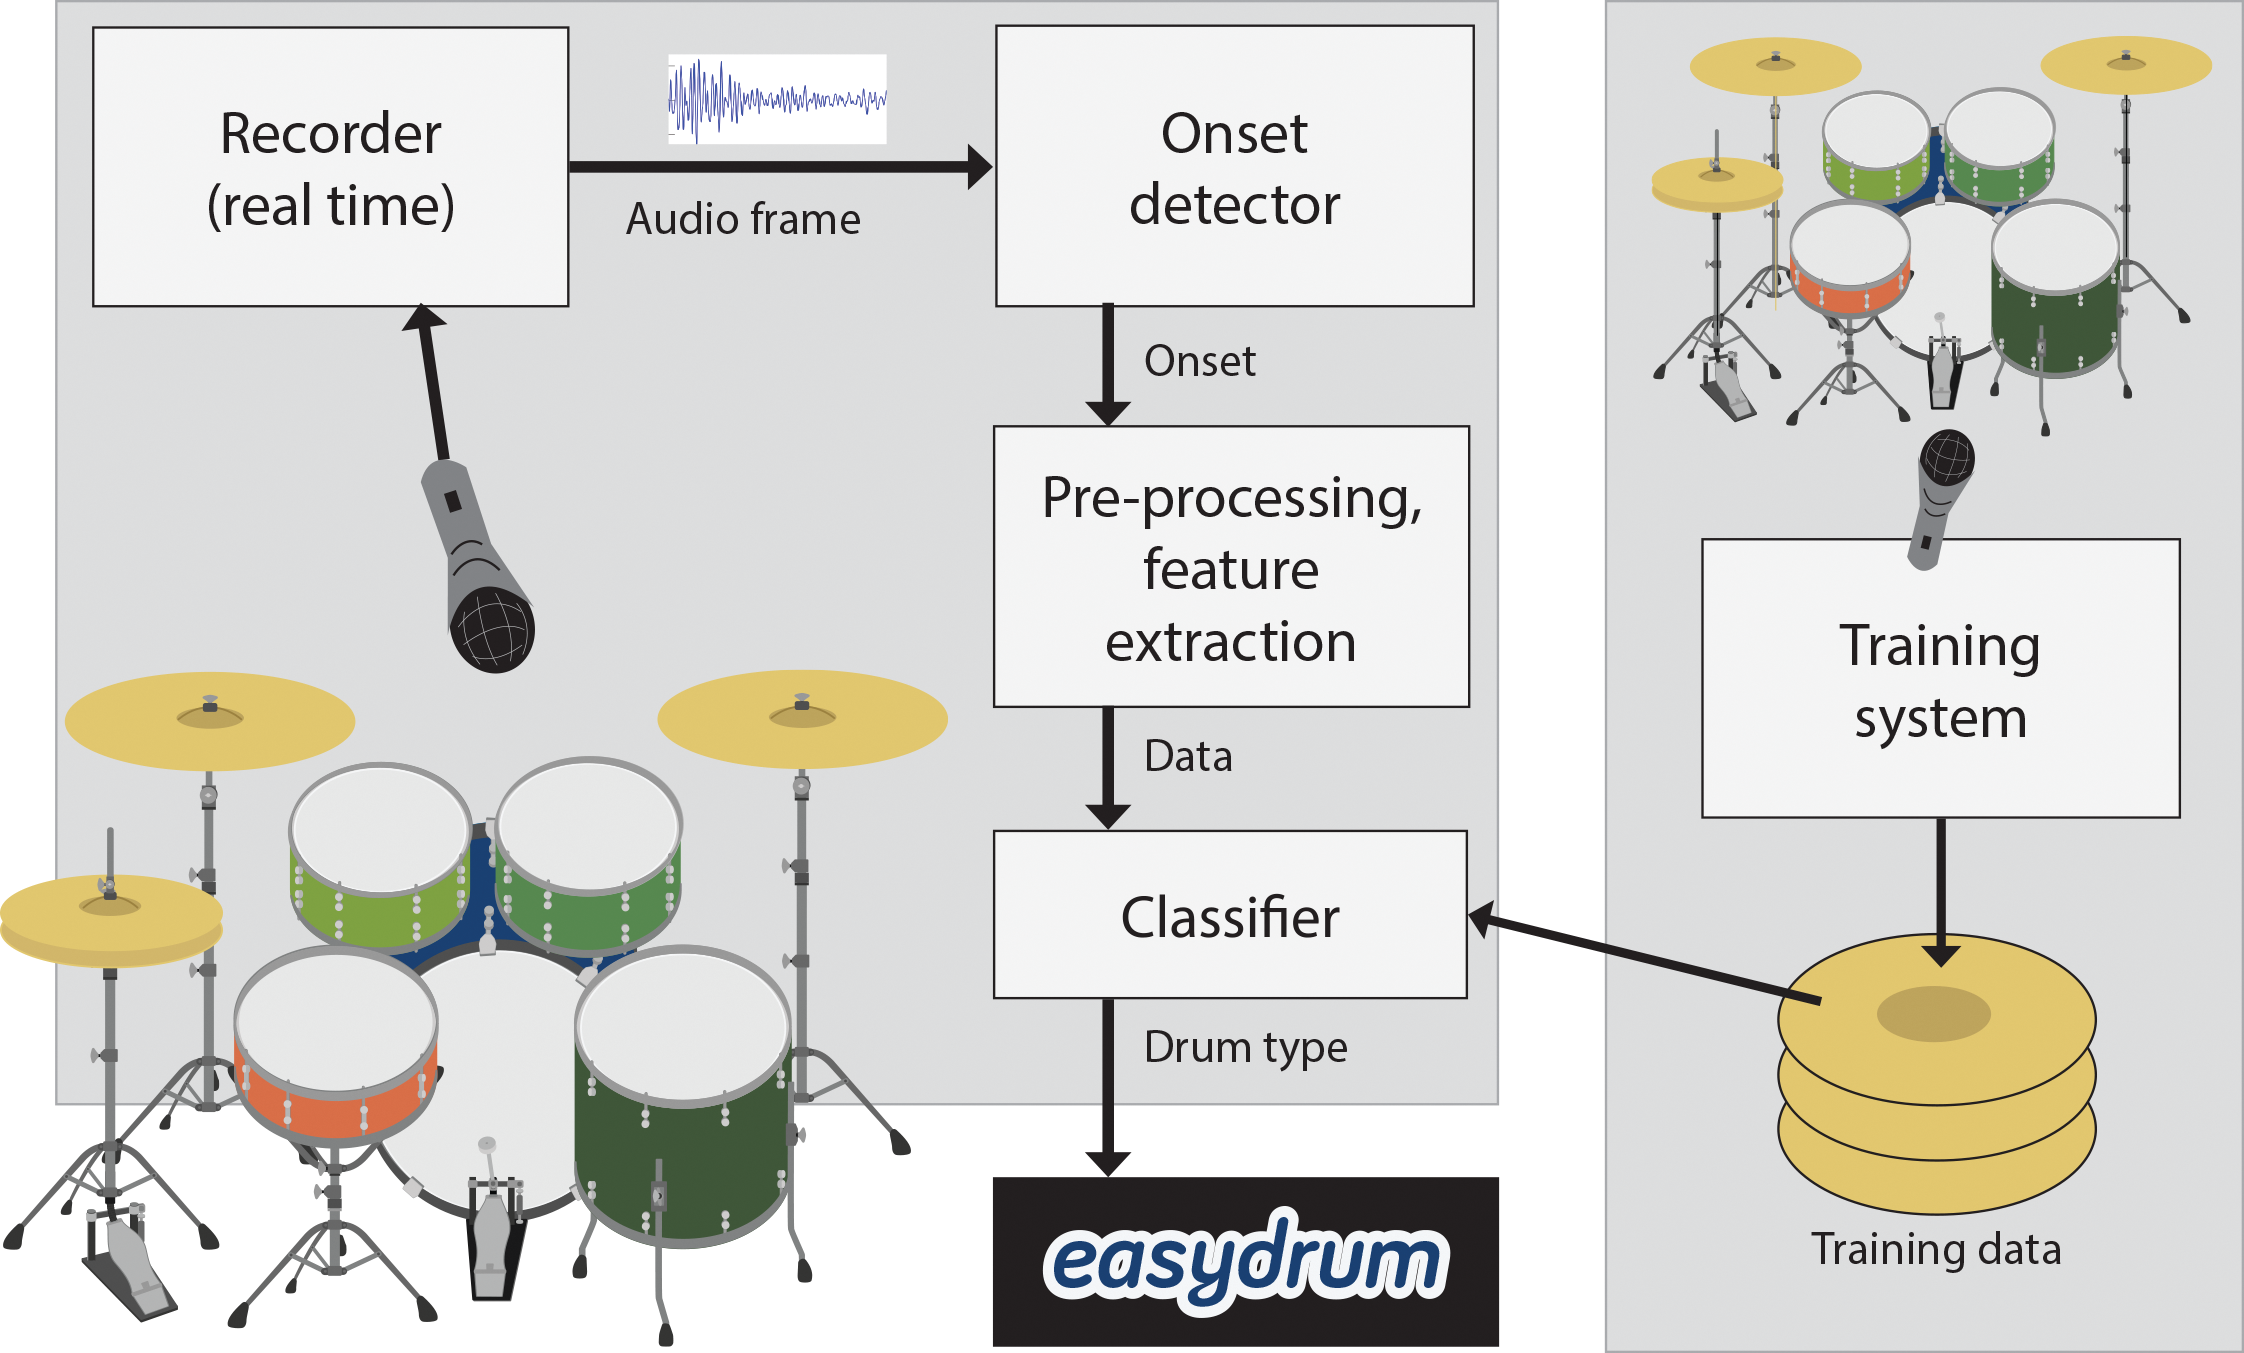
\includegraphics[width=\textwidth]{images/architecture.png}
	\caption{Drum sound analysis software architecture}
	\label{fig:architecture}
\end{figure}

With the help of the training system, the user shall be able to calibrate his drum set to use it with the software. It shall be integrated in the Easydrum drum configurator, which has already been used to configure an electronic drum set.  

The real-time drum analyzer shall be integrated in the Easydrum player. It shall consist of four steps: an audio recorder, an onset detector, a component for pre-precessing and feature extraction and a classifier. The recorder shall record small audio frames and send each of them to the onset detector. The data of each found onset shall be pre-processed for classification. Thereby, required features shall be extracted. The resulting data shall be sent to the classifier, which shall return the determined drum type and send it as an input event to the existing Easydrum player. 

In the following sections, the components required to realize this system are developed with the help of a basic drum set, which is described in section \ref{section:hardware}. An onset detection algorithm is developed that is able to run in real-time in section \ref{section:onsetdetectionmethod}, as well as two different methods for the classification of single drums and cymbals from section \ref{section:classificationSpectrumAnalysis} to section \ref{section:method2}. Furthermore, the second method is tested with simultaneous played strokes in section \ref{section:methodCombined}. The onset detection and classification algorithms are tested with MatLab\textsuperscript{\textregistered}. Finally, this chapter introduces a basic example which uses JavaScript to receive an audio stream via the browser and displays it on an HTML canvas element in section \ref{section:methodJavascript}.

\subsection{Test Drum Set and Hardware} \label{section:hardware}

For the development of the methods in this thesis, a standard drum set, a microphone, an external sound card and a laptop have been used. The used components are displayed in figure \ref{fig:components}.

\begin{SCfigure}[][h]
	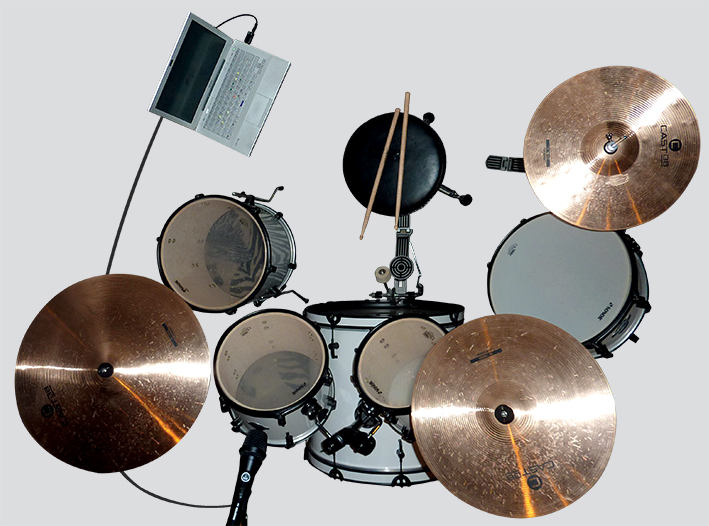
\includegraphics[width=10cm]{images/drumset/drumset_01.jpg}
	\caption{Hardware components 1. Basic drum set (Sonor SFX 11), 2. Maple leaf drumsticks, 3. Dynamic microphone (AKG P3 S), 4. External sound card (LogiLink 7.1), 5. Laptop (Sony VPCSB, 2.7 GHz, 8 GB RAM)}
	\label{fig:components} 
\end{SCfigure}

The used drum set is a basic Sonor SFX 11 drum set that consist of the following components:

\begin{itemize} 
	\item SMF 11 1816 BD WM Bass Drum 18" x 16"
	\item SMF 11 1455 SDW Snare Drum 14" x 5,5"
	\item SMF 11 1008 TT Tom Tom 10" x 8"
	\item SMF 11 1209 TT Tom Tom 12" x 9"
	\item SMF 11 1414 FT Floor Tom 14" x 14"
	\item CB8 Set 1 Cast B8 Cymbals (14" Hi-Hat, 16" Crash, 20" Ride)
	\item Maple wood drum sticks
\end{itemize}

The drum sound is recorded via a dynamic microphone (AKG P3 S) with an audio frequency bandwidth from	40 Hz to 20000 Hz. It is linked to an external USB sound card (LogiLink 7.1) via xlr to 3.5 mm headphone jack. The software runs on an 2.7 GHz Sony VAIO Laptop with 8 GB RAM and the operation system Windows 7.

\subsection{Onset Detection} \label{section:onsetdetectionmethod}

The first step of the system developed in this thesis is to detect the onsets of the drums and cymbals. Therefore, an onset detection algorithm is developed, which is able to run in real-time.

\subsubsection{Test Data}
\begin{figure}[tbp]
	\centering
	\subfloat[Bass drum]{
		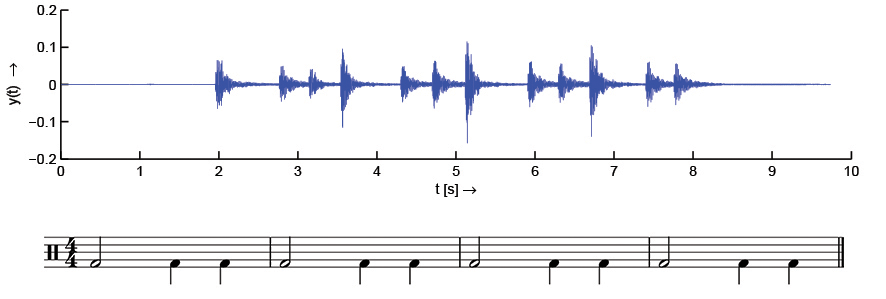
\includegraphics[width=7.3cm]{images/drumsandsheets/drum_bass.png}
	}
	\subfloat[Snare drum 1]{
		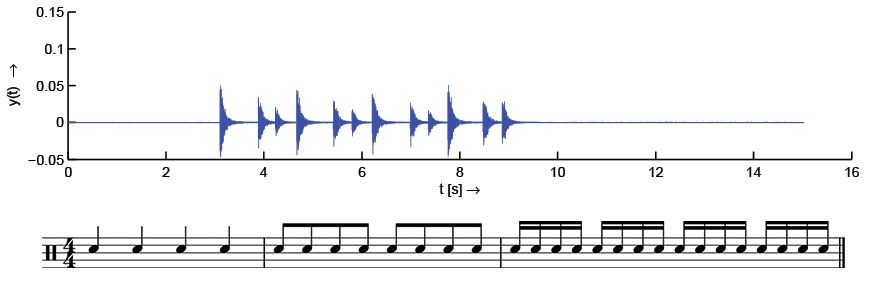
\includegraphics[width=7.3cm]{images/drumsandsheets/drum_snare.png}
	}
	\qquad
	\subfloat[Snare drum 2]{
		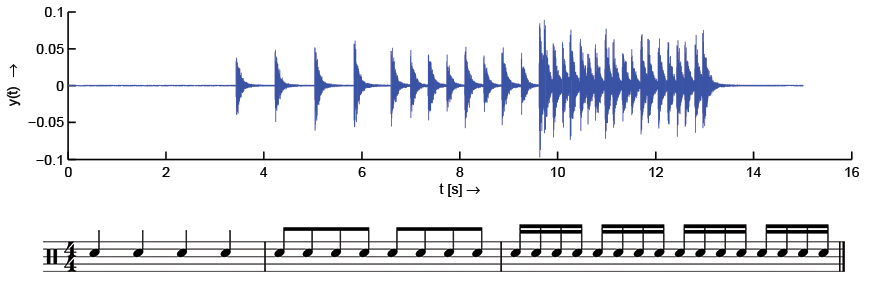
\includegraphics[width=7.3cm]{images/drumsandsheets/drum_snare2.png}
	}
	\subfloat[Tom 1]{
		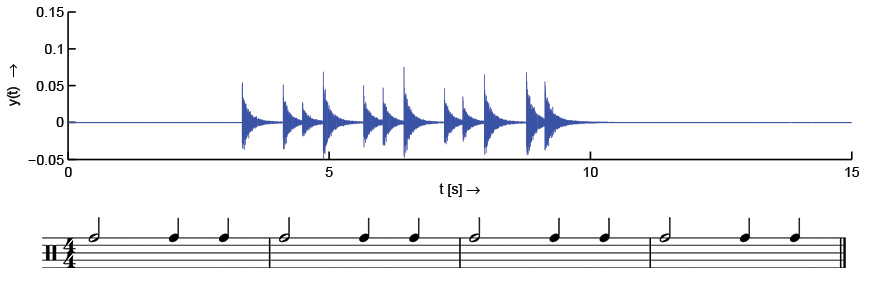
\includegraphics[width=7.3cm]{images/drumsandsheets/drum_tom1.png}
	}
	\qquad
	\subfloat[Tom 2]{
		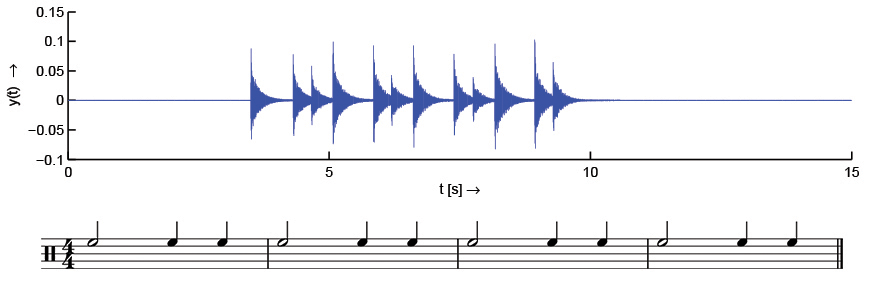
\includegraphics[width=7.3cm]{images/drumsandsheets/drum_tom2.png}
	}
	\subfloat[Tom 3]{
		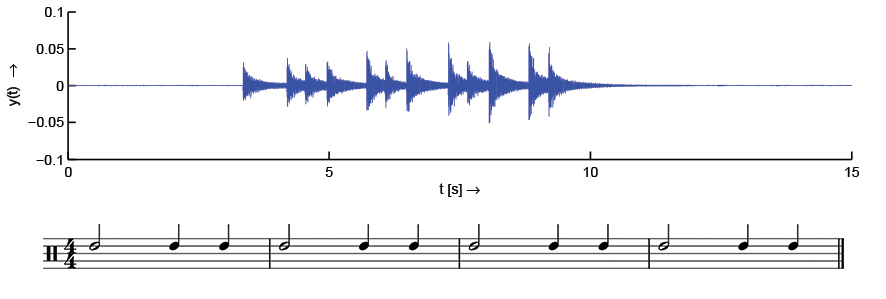
\includegraphics[width=7.3cm]{images/drumsandsheets/drum_tom3.png}
	}
	\caption{Drum loops with single drums.}
	\label{fig:recordings1}
\end{figure}

\begin{figure}[tbp]
	\centering
	\subfloat[Hi-hat closed]{
		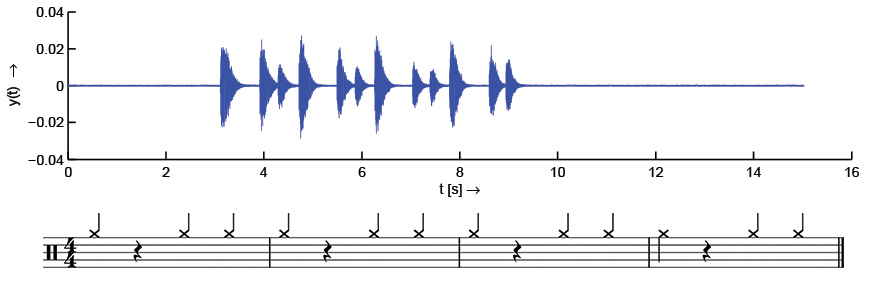
\includegraphics[width=7.3cm]{images/drumsandsheets/drum_hihatclosed.png}
	}
	\subfloat[Hi-hat open]{
		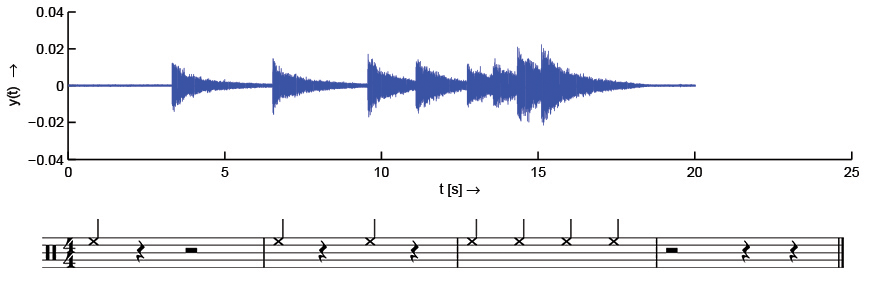
\includegraphics[width=7.3cm]{images/drumsandsheets/drum_hihatopen.png}
	}
	\qquad
	\subfloat[Crash cymbal]{
		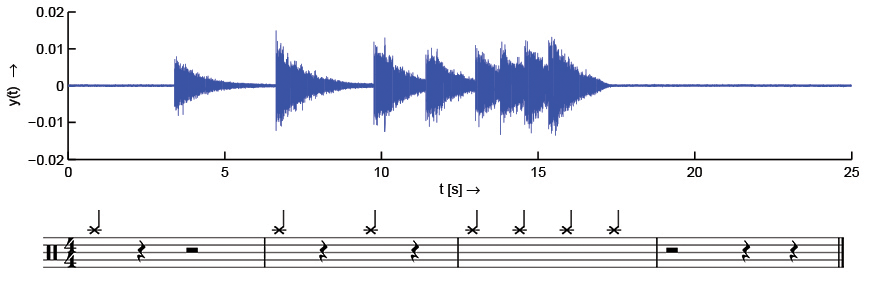
\includegraphics[width=7.3cm]{images/drumsandsheets/drum_crash.png}
	}
	\subfloat[Ride cymbal]{
		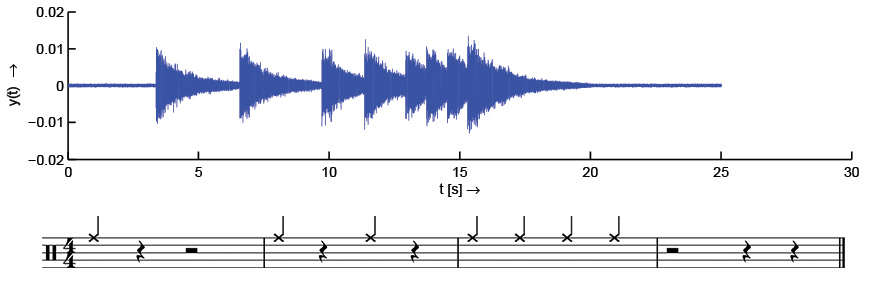
\includegraphics[width=7.3cm]{images/drumsandsheets/drum_ride.png}
	}
	\caption{Drum loops with single cymbals.}
	\label{fig:recordings2}
\end{figure}

\begin{figure}[tbp]
	\centering
	\subfloat[Loop 1]{
		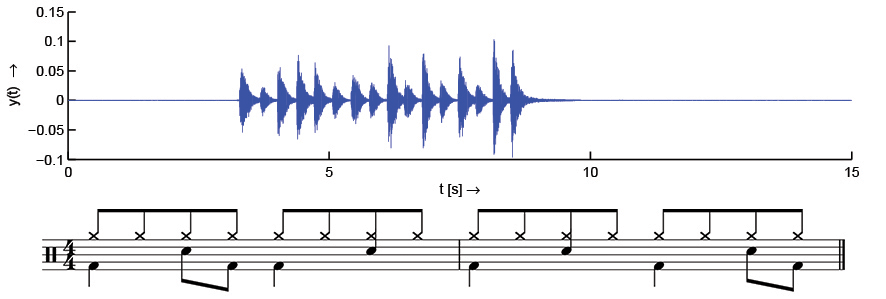
\includegraphics[width=7.3cm]{images/drumsandsheets/loop1.png}
	}
	\subfloat[Loop 2]{
		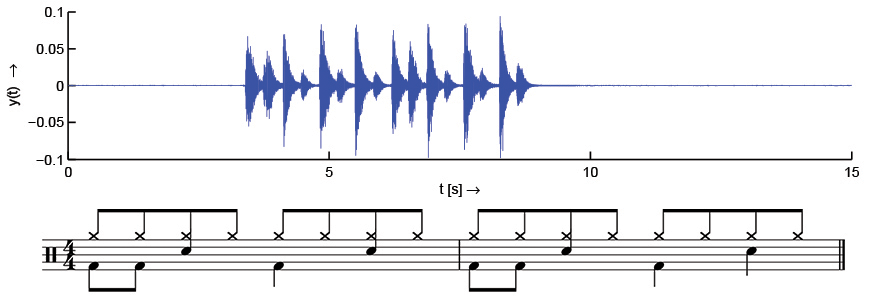
\includegraphics[width=7.3cm]{images/drumsandsheets/loop2.png}
	}
	\qquad
	\subfloat[Loop 3]{
		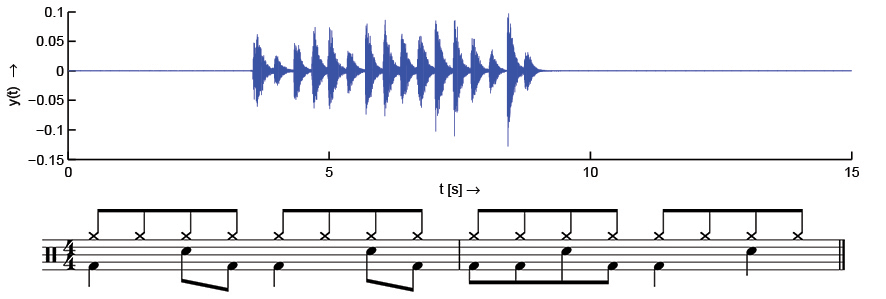
\includegraphics[width=7.3cm]{images/drumsandsheets/loop3.png}
	}
	\subfloat[Loop 4]{
		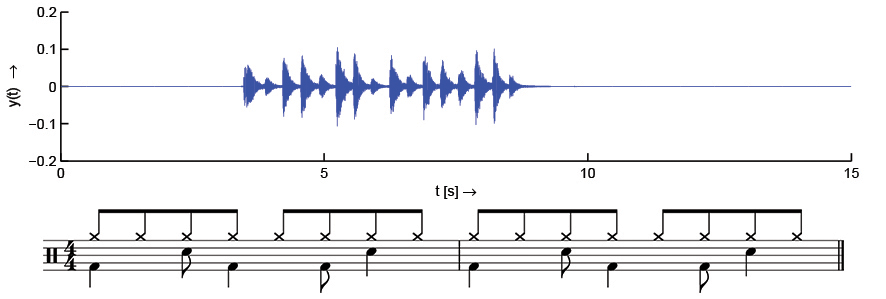
\includegraphics[width=7.3cm]{images/drumsandsheets/loop4.png}
	}
	\caption{Drum loops with bass drum, snare drum and closed hi-hat.}
	\label{fig:recordings3}
\end{figure}

\begin{figure}[tbp]
	\centering
	\subfloat[Fill-in 1 - snare drum, tom 1, tom 2, tom 3]{
		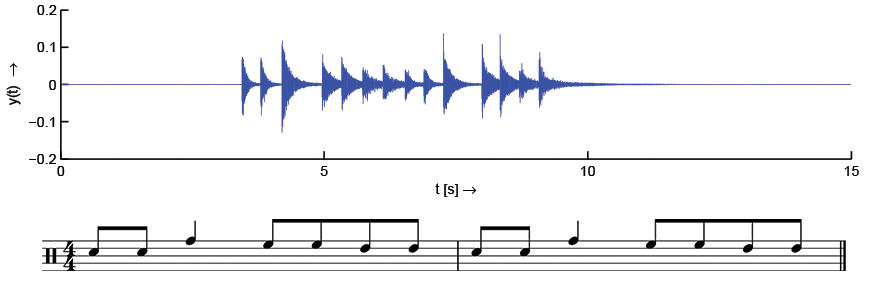
\includegraphics[width=7.3cm]{images/drumsandsheets/fillin1.png}
		\label{fig:fillin1}
	}
	\subfloat[Fill-in 2 - bass drum, snare drum, crash cymbal]{
		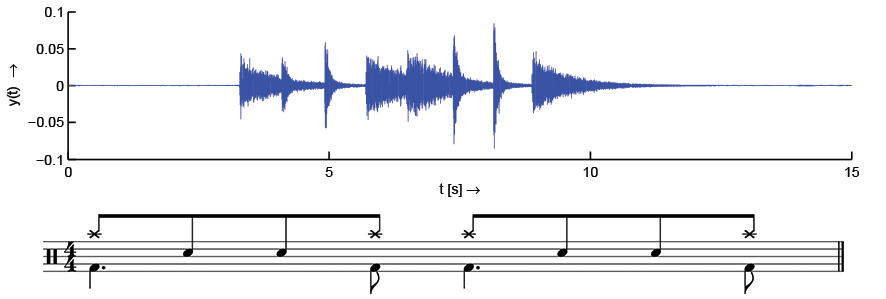
\includegraphics[width=7.3cm]{images/drumsandsheets/fillin2.png}
		\label{fig:fillin2}
	}
	\qquad
	\subfloat[Fill-in 3 - bass drum, snare drum, crash cymbal]{
		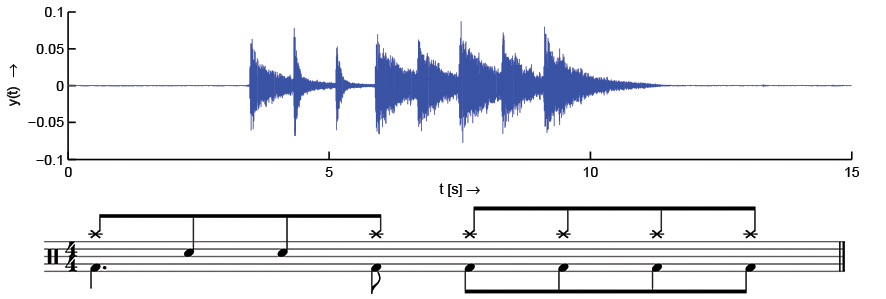
\includegraphics[width=7.3cm]{images/drumsandsheets/fillin3.png}
		\label{fig:fillin3}
	}
	\subfloat[Fill-in 4 - ride cymbal bow and bell]{
		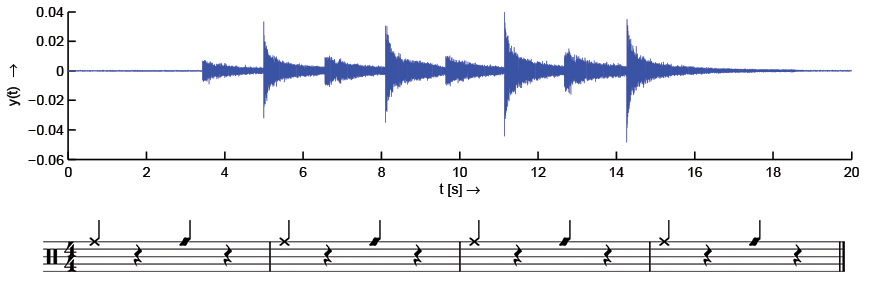
\includegraphics[width=7.3cm]{images/drumsandsheets/fillin4.png}
		\label{fig:fillin4}
	}
	\caption{Fill-ins.}
	\label{fig:recordings4}
\end{figure}

To evaluate the onset detection algorithm developed in the following, there are different short drum loops recorded. They are further used to analyze the waveforms of the different drums and cymbals. Figures \ref{fig:recordings1} to \ref{fig:recordings4} show the audio signals of these recordings with appropriate sheets. The sound files include a recording for each used drum and cymbal in which they are played at different intervals (figure \ref{fig:recordings1} and \ref{fig:recordings2}). For the snare drum there is an additional recording in which it is played faster. Moreover, four drum loops and four fill-ins were recorded. The drum loops (figure \ref{fig:recordings3}) contain common drum rhythms including the bass drum, the snare drum and the closed hi-hat. One of the fill-ins (figure \ref{fig:fillin1}) contains the snare drums and the three tom toms. Two of the fill-ins (figures \ref{fig:fillin2} and \ref{fig:fillin3}) contain the bass drum, the snare drum and the crash cymbal, whereas the crash cymbal is played together with the bass drum. The last fill-in (figure \ref{fig:fillin4}) contains the ride cymbal with rim and bell played alternately.

\subsubsection{Analysis of Drum Recordings}

Before the onset detection algorithm is developed, the recordings are analyzed to figure out which characteristics need to be considered for onset detection. Thereby, it is observed that every stroke on a drum or cymbal produces an explicit rise in amplitude. This rise in energy is followed by the decay of the signal. Hence, the algorithm only needs to be based on the audio wave. There is no need to consider the frequency spectrum. This way, the computing time can be reduced. 

To be able to find the onsets only on the basis of the audio wave, the forms of the different drum strokes need to be regarded. Different drum types vary in their attack and decay time. The decay of all drums shows an inversely proportional form. The cymbals, except the closed hi-hat, decay much slower than the drums. 

The opened hi-hat, the crash cymbal and the ride cymbal show similar waveforms. They decay much slower than the closed hi-hat and the drums. The attack time of these cymbals is nearly zero. The decay can show vibrations. Thus, in the decaying phase of a tone the amplitudes can rise without a new stroke. The crash cymbal shows most vibrations, the opened hi-hat the least. The closed hi-hat can also show vibrations, but it decays much faster. In contrast to the other cymbals, it has a higher attack time. This means that its amplitude rises for a short time period after the onset. This phenomenon can also be observed for the bass drum. It even has a longer attack time than the hi-hat. Furthermore, there are more vibrations, whilst the decay time is similar. The remaining drums show no significant attack time or vibrations. While the tom toms decay slower than the bass drum, the snare drum shows the shortest decay time of all considered drums and cymbals. It decays slightly shorter than the hi-hat and bass drum. 

Hence, for the onset detector it is significant to support different decay times, and not to detect vibrations and rising amplitudes during the attack as onsets.

\newpage
\subsubsection{Method}

The developed onset detection algorithm is based on the algorithm in \autocite{Schloss:1985}, which is described in section \ref{section:OnsetDetectionSchloss}. Schloss uses a fast and simple algorithm which only considers the amplitude envelope of the audio wave. As a stroke on a drum always produces an increase in the amplitude envelope, this is a good method to achieve a short computing time. Moreover, Schloss considers subsequent frames of an audio file to detect the onsets. Thus, the algorithm described in \autocite{Schloss:1985} provides the required features to run in real-time.

Hence, based on the method of Schloss, the algorithm developed in this thesis scans subsequent recorded frames for sudden rises in the amplitude of the audio wave. Therefore, the actual frame is compared to the mean of a given number of preceding frames. The algorithm is able to run in real-time. It is implemented as a MatLab\textsuperscript{\textregistered} class called \textit{DetectOnset}. An UML diagram of the class is shown in figure \ref{fig:onsetDetectorUML}.

\begin{figure}[htb]
	\centering
	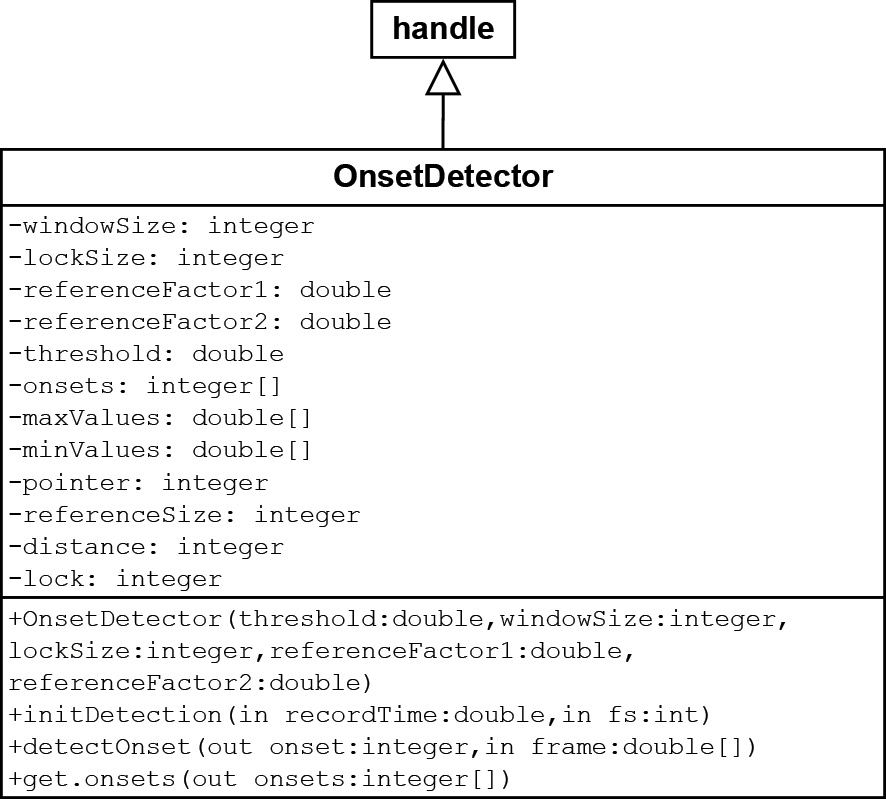
\includegraphics[width=7.5cm]{images/UML/onsetDetectorUML.png}
	\caption{UML diagram of the onset detector}
	\label{fig:onsetDetectorUML}
\end{figure}

The class has the properties \lstinline{threshold} (data type double), \lstinline{windowSize} (data type integer), \lstinline{lockSize} (data type integer), \lstinline{referenceFactor1} (data type double), \lstinline{referenceFactor2} (data type double), \lstinline{onsets} (vector of data type integer), \lstinline{maxValues} (vector of data type double), \lstinline{minValues} (vector of data type double), \lstinline{pointer} (data type integer), \lstinline{referenceSize} (data type integer), \lstinline{distance} (data type integer) and \lstinline{lock} (data type integer).

\begin{sloppypar}
The property values for \lstinline{threshold}, \lstinline{windowSize},  \lstinline{lockSize}, \lstinline{referenceFactor1} and \lstinline{referenceFactor2} are set by the constructor. Whereas the threshold always needs to be specified, there are default values for the remaining parameters. If they are not passed, the values are set to \lstinline{windowSize=512}, \lstinline{lockSize=8}, \lstinline{referenceFactor1=1} and \lstinline{referenceFactor2=0.5}. The parameter \lstinline{referenceFactor1} should contain a value greater than one and \lstinline{referenceFactor2} a value between zero and one.
\end{sloppypar}

The parameter \lstinline{threshold} defines the minimum amplitude that can be declared as an onset. With the help of this parameter the algorithm defining the noise of the recording or low background sounds as onsets is avoided. For testing method developed in this thesis, the threshold is defined by analyzing a frame that only contains noise. The maximum value of this frame multiplied with the factor five is chosen as the threshold value. Thus, an onset must have the minimum amplitude of five times the maximum noise amplitude.

The parameter \lstinline{windowSize} defines the size of the frames in which the audio file is segmented. 

The parameter \lstinline{lockSize} defines the size of the lock, which is set after every onset. This lock prohibits to find two onsets in an interval of a given number of frames after an onset. It is needed because the amplitude rises a certain time after the onset. Furthermore, especially the amplitude of a cymbal can be very unstable. Thus, in this time interval there should be no more onset detected because it would be produced by the same stroke. 

The vectors \lstinline{minValues} and \lstinline{maxValues} are used to save the minimum and maximum amplitudes of each frame. 

The property \lstinline{pointer} saves the number of recently processed frames during the runtime of the current onset detection process. Thus, it points to the index of the last added value in the vectors \lstinline{minValues} and \lstinline{maxValues}.

The properties \lstinline{referenceSize}, \lstinline{distance} and \lstinline{lock} store non-static values, which are changing during the runtime of the algorithm. 

The property \lstinline{distance} saves the number of frames from the currently considered frame to the frame with the last found onset. 

The property \lstinline{referenceSize} defines the number of preceding frames considered when analyzing a frame for an onset. It is used to calculate the values of \lstinline{minReference} and \lstinline{maxReference}, which save two thresholds. To be declared as an onset, the frame must contain an amplitude smaller than \lstinline{minReference} and an amplitude greater than \lstinline{maxReference}. The maximum amplitude is calculated by the mean of all maxima in the preceding frames multiplied with the value of \lstinline{referenceFactor1}, which is transferred to the onset detector as a parameter. The minimum amplitude is calculated in the same way, with the difference that the minimum values are used. Thereby, \lstinline{minReference} may not be greater than \lstinline{-threshold} and \lstinline{maxReference} may not be smaller than \lstinline{threshold}. Listing \ref{lst:onset1} shows the appropriate MatLab\textsuperscript{\textregistered} code.

%[\label{listing:onset1}]
\begin{lstlisting}[caption={Calculation of minReference and maxReference},label={lst:onset1}]
minReference= ...
		mean(obj.minValues(obj.pointer-obj.referenceSize-1:obj.pointer-1)) ...
		*obj.referenceFactor1;
maxReference= ...
		mean(obj.maxValues(obj.pointer-obj.referenceSize-1:obj.pointer-1)) ...
		*obj.referenceFactor1;

if (minReference > obj.threshold) minReference=-obj.threshold; end
if (maxReference < obj.threshold) maxReference=obj.threshold; end  
\end{lstlisting}

%- Die Variable lock definiert eine Sperre. Ist die Sperre aktiviert kann kein Onset vorliegen. Nachdem ein Onset gefunden wurde wird lock gleich dem Parameter lock_size gesetzt. Nach jedem Frame wird lock um eins vermindert. Nur wenn lock null ist, kann ein Onset gefunden werden.
The property \lstinline{lock} saves the status of the lock. It is set to the size of the parameter \lstinline{lockSize} after an onset is detected and otherwise downsized by one. The minimum value of \lstinline{lock} is zero. If the value is greater than zero, the lock is activated and no onset can be found. Thus, an onset can only be detected if \lstinline{lock} is equal to zero.   

To calculate the value for \lstinline{referenceSize}, the parameter \lstinline{referenceFactor2} is needed. It defines the percentage of frames from the currently considered frame to the frame with the last onset. Within the MatLab\textsuperscript{\textregistered} function the value is calculated by \lstinline{referenceSize=ceil(distance*referenceFactor2)}. Hence, the higher the distance to the last onset, the higher the value for \lstinline{referenceSize}. After an onset has been found, \lstinline{referenceSize} is reset to one.

%Die reference_size wird größer, je weiter der letzte Onset zurückliegt. Es werden nur Frames betrachtet, die nach dem letzten Onset liegen. Je weiter dieser zurück liegt, desto mehr Frames liegen also zwischen letztem Onset und gerade analysiertem Frame, desto mehr Frames können betrachtet werden, um den Mittelwert zu berechnen. Da die Amplitude nach einem Onset langsam abnimmt, muss auch der Referenzwert für einen neuen Onset abnehmen. Der als Referenzwert berechnete Mittelwert darf also nicht zu groß werden, da dadurch unter Umständen ein Onset mit geringerer Amplitude als der vorangehende nicht entdeckt wird. Dies wird dadurch vermieden, dass bei der Berechnung von min_reference/max_reference nicht alle Frames bis zum letzten Onset genutzt werden. Die Anzahl der Frames, die betrachtet werden wird durch ceil(distance/reference_denominator) berechnet.
The variation of the property \lstinline{referenceSize} is a decisive part of the algorithm. It is based on the fact that the amplitude decays inversely proportional after an onset. Thereby, some stroke types decay faster than others. Hence, the higher the distance to the last onset, the slower the sound decays and the smaller the amplitude difference when comparing the actual frame with the mean of the preceding ones. By rising the number of frames for comparison, the calculated mean values do also rise. Thus, the amplitude rise has to be greater than it had to be if it would be compared with less frames. This way, the detection of small rises in amplitude, which are caused by vibrations, as false onsets is avoided. Contrariwise, the comparison may also not include too many frames because if the mean value is too high, onsets with lower amplitudes than the preceding one would not be detected.

The vector \lstinline{onsets} saves the positions of all found onsets. It can be read with the help of the  getter function \lstinline{onsets=get.onsets(obj)}.

The function \lstinline{start} needs to be called to initialize a new onset detection process. It is used both before the start of the first onset detection process and to reset the onset detector to begin the detection for a new recording. The function receives the parameters \lstinline{recordTime} and \lstinline{fs}. 

The parameter \lstinline{recordTime} is the period of time in seconds that the onset detection process will be running. In the final system this time will be the duration of the played exercise. If an audio file is scanned it is the duration of the record. The parameter \lstinline{fs} is the sampling rate of the audio input in frames per second. The parameters are needed here to predefine the length of the vectors \lstinline{minValues} and \lstinline{maxValues} and thus to allocate the appropriate memory. It is calculated by \lstinline{ceil(recordTime/(obj.windowSize/fs))}. Further on, the \lstinline{start} function sets the values for the properties \lstinline{pointer}, \lstinline{distance} and \lstinline{lock} to zero and the value for \lstinline{referenceSize} to one. 

After the onset detector is started, the function \lstinline{detectOnset}, which is the essential part of the onset detection algorithm, has to be called for every incoming frame. It receives the audio data as input argument, and if an onset is found, it returns the position of the sample containing the onset. The position is calculated by \lstinline{obj.pointer*obj.windowSize+maxIdx}, whereas \lstinline{maxIdx} defines the index of the actual frames maximum amplitude. If there is no onset found the function returns zero.

The function \lstinline{detectOnset} scans each frame for an onset as follows:

\begin{enumerate}
	\item The variable \lstinline{onset} is defined and set to zero.
	\item \lstinline{pointer} is increased by one.
	\item The minimum and maximum amplitudes of the particular frame are identified and stored in the arrays \lstinline{minValues} and \lstinline{maxValues}. The index of the maximum amplitude is saved as the variable \lstinline{maxIdx}.
	\item If the actual value of the property \lstinline{pointer} is greater than the value of \lstinline{referenceSize+1}, the function proceeds with the next step, otherwise the function returns.
	\item The variables \lstinline{minReference} and \lstinline{maxReference} are calculated as shown in listing \ref{lst:onset1}.
	\item  If the minimum value of the considered frame is smaller than \lstinline{minReference}, the maximum value higher than \lstinline{maxReference} and there is no lock set, the function proceeds with step 6a, otherwise it proceeds with step 6b.
	\begin{enumerate}
		\item The actual maximum position is declared as an onset. The onsets position is calculated by \lstinline{obj.pointer*obj.windowSize+maxIdx}. It is saved in the variable \lstinline{onset} and appended to the vector \lstinline{onsets}. Further on, the property \lstinline{referenceSize} is reset to one, \lstinline{distance} to zero and \lstinline{lock} to \lstinline{lockSize}. It is proceeded with step 7.
		
		\item The property \lstinline{distance} is set to one and the property \lstinline{referenceSize} is calculated by \lstinline{ceil(obj.distance*obj.referenceFactor2)}. It is proceeded with step 7.
	\end{enumerate}
	\item If the property \lstinline{lock} is	greater than zero, it is decreased by one.				
\end{enumerate}

The entire \lstinline{detectOnset} function is displayed in listing \ref{lst:detectOnset}.

\begin{lstlisting}[caption={detectOnset},label={lst:detectOnset}]
function onset=detectOnset(obj,frame)
	onset=0;
	obj.pointer=obj.pointer+1;
  [maxValue,maxIdx]=max(frame);
	obj.minValues(obj.pointer)=min(frame);
	obj.maxValues(obj.pointer)=maxValue;
	
	if obj.pointer>obj.referenceSize+1 
		minReference=  ...
				mean(obj.minValues(obj.pointer-obj.referenceSize-1:obj.pointer-1)  ...
				*obj.referenceFactor1;
		maxReference=  ...
				mean(obj.maxValues(obj.pointer-obj.referenceSize-1:obj.pointer-1))  ...
				*obj.referenceFactor1;

		if (minReference > obj.threshold) minReference = -obj.threshold; end
		if (maxReference < obj.threshold) maxReference = obj.threshold; end  

		if (obj.minValues(obj.pointer) < minReference  ...
		&& obj.maxValues(obj.pointer) > maxReference && obj.lock==0) 
			onset=obj.pointer*obj.windowSize+maxIdx; 
			obj.onsets=[obj.onsets,onset];
			obj.referenceSize=1;
			obj.distance=0;
			obj.lock=obj.lockSize;
		else
			obj.distance=obj.distance+1;
			obj.referenceSize=ceil(obj.distance*obj.referenceFactor2);
		end
		if obj.lock > 0
			obj.lock=obj.lock-1;
		end            
	end	
end
\end{lstlisting}


\subsubsection{Tests}

To test the algorithm, it is applied to the previously recorded sound files. These recordings contain a total of 226 onsets.

A MatLab function reads in the files and splits them into frames with the size of a given value for the parameter \lstinline{windowSize}. For each record, an instance of the class \lstinline{OnsetDetector} is created and its \lstinline{start} function is called. Subsequent, the appropriate frames are sent to the \lstinline{onsetDetection} function. The resulting array of onsets for each record is drawn to a figure. To improve the hit-rate, the parameters \lstinline{windowSize}, \lstinline{lockSize}, \lstinline{referenceFactor1} and \lstinline{referenceFactor2} are varied. 

It is important to choose a convenient window size to enable the algorithm to run in real-time. If the frame size is too small, the algorithm needs too long to perform during the runtime. If it is too large, the resolution is too small and a detected onset is returned too late. Moreover, onsets can be missed because two onsets are located within the same frame. It also needs to be considered that the number of onsets can rise when choosing a small frame size because vibrations are split to several frames and thus declared as onsets. The best results have been gained with a frame size of 512 samples, which equals 11.6 ms. The lock size is set to 8. Thus, there is a lock for a total of 4096 ($8*512$) samples. This equals 92 ms during which no further onset can be detected. The value for \lstinline{referenceFactor1} is found to be effective between 1.4 and 1.6 in combination with \lstinline{referenceFactor2} between 0.4 and 0.5. 

The best results have been gained by using the values 1.52 for \lstinline{referenceFactor1} and 0.4 for \lstinline{referenceFactor2}. There is one onset missing and one false positive onset. The results are shown in figure \ref{fig:onsetTest1}. The missing onset is a stroke on the snare drum in figure \ref{fig:onsetTest1_1}. At this part of the record the snare drum is played fast. The stroke is to close to the preceding one and the minimum amplitude of the stroke is much lower, but the used factors \lstinline{referenceFactor1=1.52} and \lstinline{referenceFactor2=0.4} produce a lower value for \lstinline{minReference}, here. Hence, the stroke cannot be detected. The false positive is a stroke on the crash cymbal, the cymbal which creates the strongest vibrations. At the point where the false onset is detected the amplitude rises even higher than at the onset itself. Thus, the calculated values for \lstinline{minReference} are too low and for \lstinline{maxReference} too high, which causes the false detection of the onset. The stroke is placed in figure \ref{fig:onsetTest1_2}.

\begin{sloppypar}
Figure \ref{fig:onsetTest2} shows the results with the use of the factors \lstinline{referenceFactor1=1.45} and \lstinline{referenceFactor2=0.45}. With these lower factors the detection of all onsets can be achieved, but the number of false detected onsets rises to five. The results are shown in figure \ref{fig:onsetTest2}. Contrarily, trying to avoid false onsets leads to a rise in the number of missing ones. To test this, the factors are set to \lstinline{referenceFactor1=1.6} and \lstinline{referenceFactor2=0.5}. The results are displayed in figure \ref{fig:onsetTest3}. There are no false onsets, but four of the onsets are not detected by the algorithm.
\end{sloppypar}

\begin{figure}[bp]
	\centering
	\subfloat[Bass drum]{
		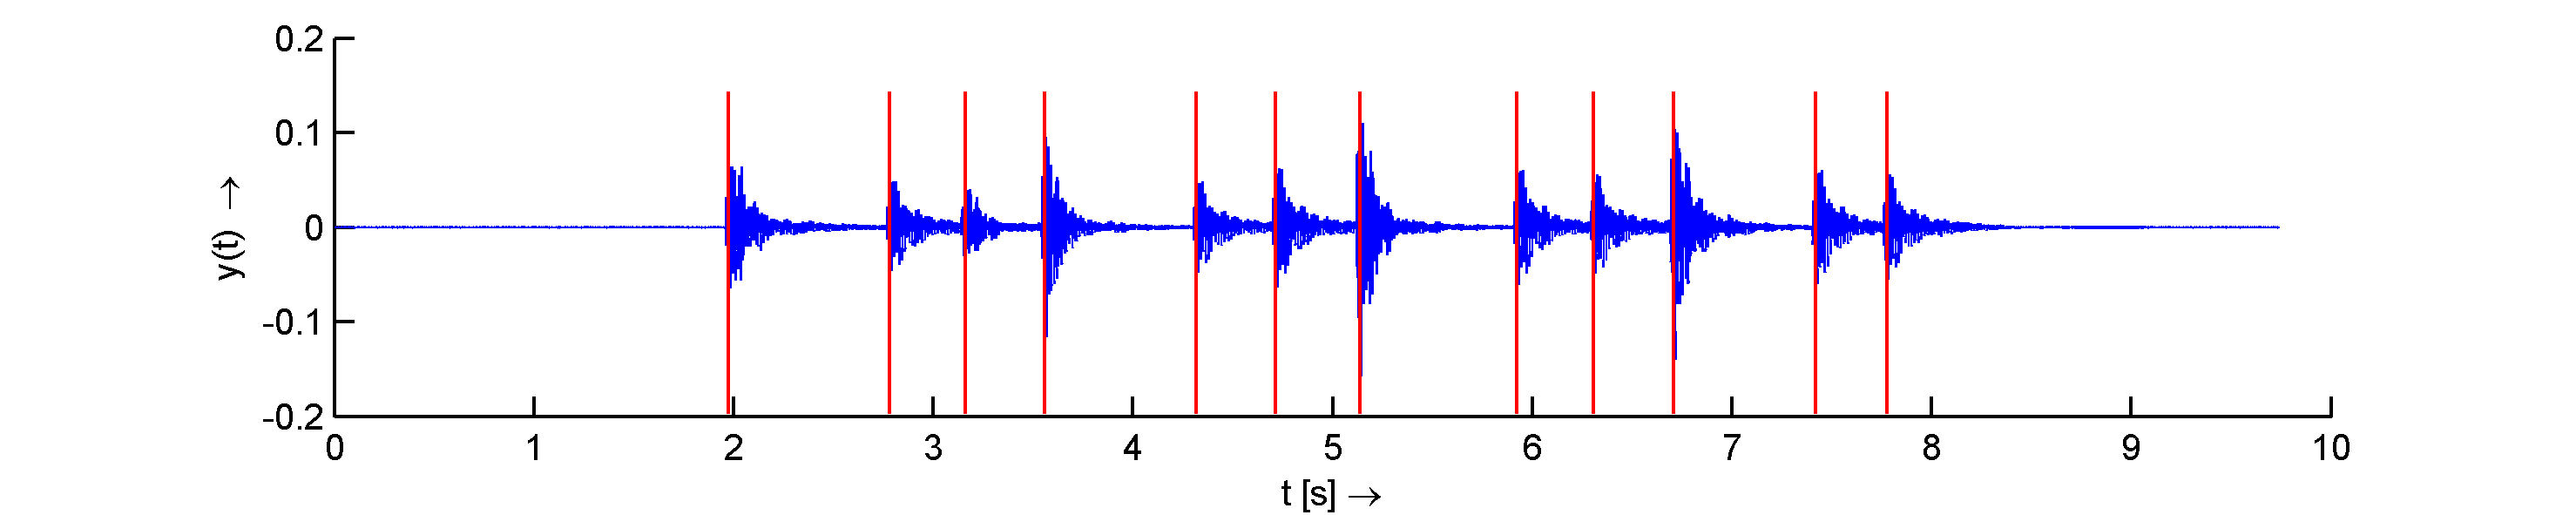
\includegraphics[width=7cm]{images/onsettest/1/drum_bass.png}
	}
	\subfloat[Snare drum 1]{
		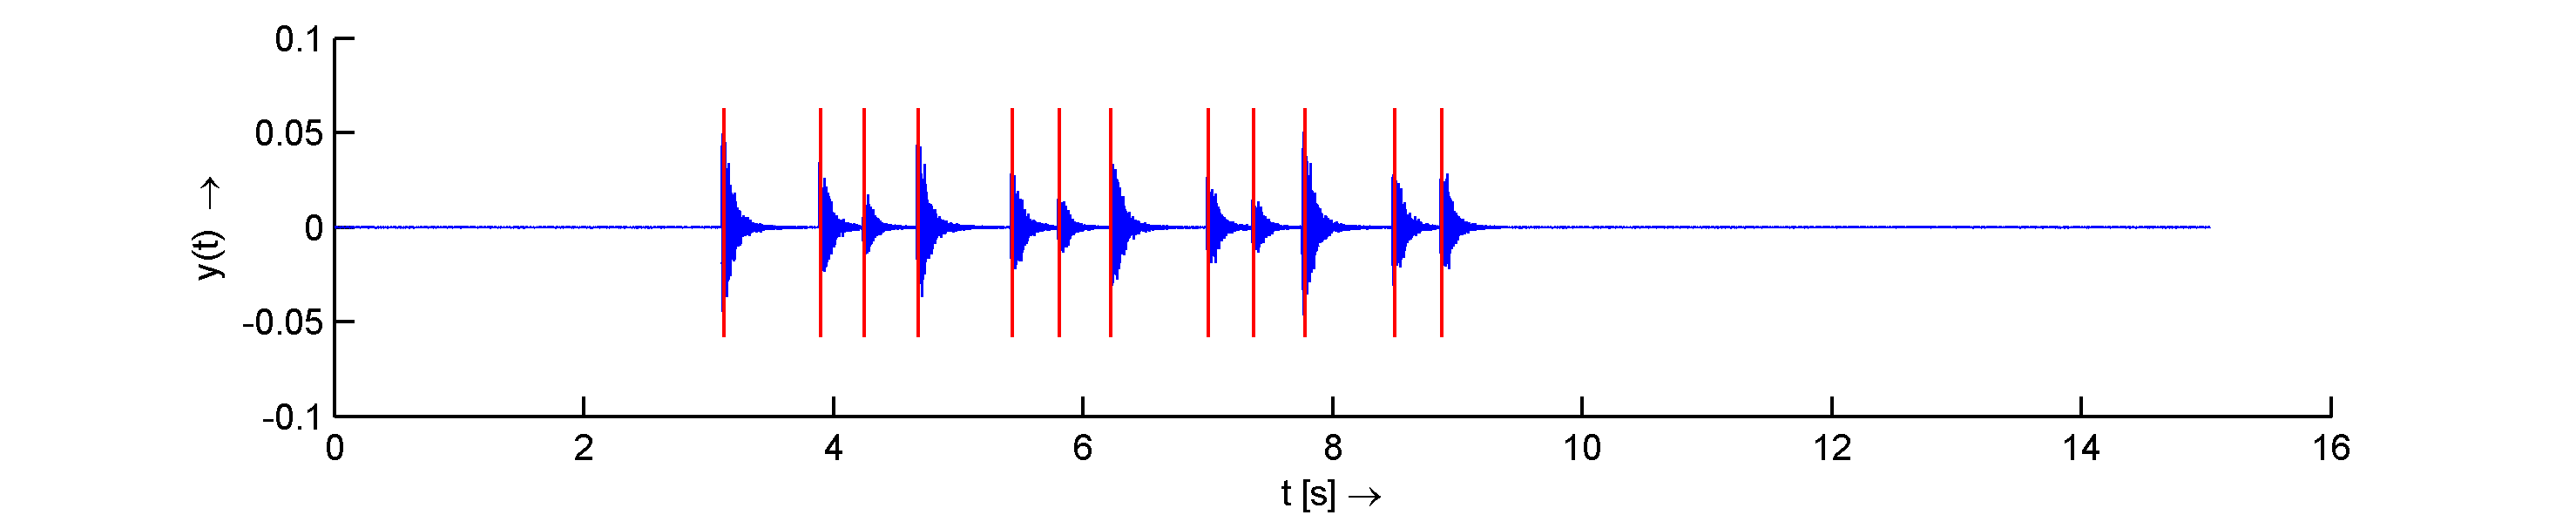
\includegraphics[width=7cm]{images/onsettest/1/drum_snare.png}
	}
	\qquad
	\subfloat[Snare drum 2]{
		\includegraphics[width=7cm]{images/onsettest/1/drum_snare2.png}
	\label{fig:onsetTest1_2}
	}
	\subfloat[Tom 1]{
		\includegraphics[width=7cm]{images/onsettest/1/drum_tom1.png}
	}
	\qquad
	\subfloat[Tom 2]{
		\includegraphics[width=7cm]{images/onsettest/1/drum_tom2.png}
	}
	\subfloat[Tom 3]{
		\includegraphics[width=7cm]{images/onsettest/1/drum_tom3.png}
	}
	\qquad
	\subfloat[Hi-hat closed]{
		\includegraphics[width=7cm]{images/onsettest/1/drum_hihatclosed.png}
	}
	\subfloat[Hi-hat open]{
		\includegraphics[width=7cm]{images/onsettest/1/drum_hihatopen.png}
	}
	\qquad
	\subfloat[Crash cymbal]{
		\includegraphics[width=7cm]{images/onsettest/1/drum_crash.png}
	 \label{fig:onsetTest1_1}
	}
	\subfloat[Ride cymbal]{
		\includegraphics[width=7cm]{images/onsettest/1/drum_ride.png}
	}
	\qquad
	\subfloat[Loop 1]{
		\includegraphics[width=7cm]{images/onsettest/1/loop1.png}
	}
	\subfloat[Loop 2]{
		\includegraphics[width=7cm]{images/onsettest/1/loop2.png}
	}
	\qquad
	\subfloat[Loop 3]{
		\includegraphics[width=7cm]{images/onsettest/1/loop3.png}
	}
	\subfloat[Loop 4]{
		\includegraphics[width=7cm]{images/onsettest/1/loop4.png}
	}
	\qquad
	\subfloat[Fill-in 1 - snare drum, tom 1, tom 2, tom 3]{
		\includegraphics[width=7cm]{images/onsettest/1/fillin1.png}
	}
	\subfloat[Fill-in 2 - bass drum, snare drum, crash cymbal]{
		\includegraphics[width=7cm]{images/onsettest/1/fillin2.png}
	}
	\qquad
	\subfloat[Fill-in 3 - bass drum, snare drum, crash cymbal]{
		\includegraphics[width=7cm]{images/onsettest/1/fillin3.png}
	}
	\subfloat[Fill-in 4 - ride cymbal bow and bell]{
		\includegraphics[width=7cm]{images/onsettest/1/fillin4.png}
	}
	\caption{Onset detection test 1.}
	\label{fig:onsetTest1}
\end{figure}


\begin{figure}[bp]
	\centering
	\subfloat[Bass drum]{
		\includegraphics[width=7cm]{images/onsettest/2/drum_bass.png}
	}
	\subfloat[Snare drum 1]{
		\includegraphics[width=7cm]{images/onsettest/2/drum_snare.png}
	}
	\qquad
	\subfloat[Snare drum 2]{
		\includegraphics[width=7cm]{images/onsettest/2/drum_snare2.png}
	}
	\subfloat[Tom 1]{
		\includegraphics[width=7cm]{images/onsettest/2/drum_tom1.png}
	}
	\qquad
	\subfloat[Tom 2]{
		\includegraphics[width=7cm]{images/onsettest/2/drum_tom2.png}
	}
	\subfloat[Tom 3]{
		\includegraphics[width=7cm]{images/onsettest/2/drum_tom3.png}
	}
	\qquad
	\subfloat[Hi-hat closed]{
		\includegraphics[width=7cm]{images/onsettest/2/drum_hihatclosed.png}
	}
	\subfloat[Hi-hat open]{
		\includegraphics[width=7cm]{images/onsettest/2/drum_hihatopen.png}
	}
	\qquad
	\subfloat[Crash cymbal]{
		\includegraphics[width=7cm]{images/onsettest/2/drum_crash.png}
	}
	\subfloat[Ride cymbal]{
		\includegraphics[width=7cm]{images/onsettest/2/drum_ride.png}
	}
	\qquad
	\subfloat[Loop 1]{
		\includegraphics[width=7cm]{images/onsettest/2/loop1.png}
	}
	\subfloat[Loop 2]{
		\includegraphics[width=7cm]{images/onsettest/2/loop2.png}
	}
	\qquad
	\subfloat[Loop 3]{
		\includegraphics[width=7cm]{images/onsettest/2/loop3.png}
	}
	\subfloat[Loop 4]{
		\includegraphics[width=7cm]{images/onsettest/2/loop4.png}
	}
	\qquad
	\subfloat[Fill-in 1 - snare drum, tom 1, tom 2, tom 3]{
		\includegraphics[width=7cm]{images/onsettest/2/fillin1.png}
	}
	\subfloat[Fill-in 2 - bass drum, snare drum, crash cymbal]{
		\includegraphics[width=7cm]{images/onsettest/2/fillin2.png}
	}
	\qquad
	\subfloat[Fill-in 3 - bass drum, snare drum, crash cymbal]{
		\includegraphics[width=7cm]{images/onsettest/2/fillin3.png}
	}
	\subfloat[Fill-in 4 - ride cymbal bow and bell]{
		\includegraphics[width=7cm]{images/onsettest/2/fillin4.png}
	}
	\caption{Onset detection test 2.}
	\label{fig:onsetTest2}
\end{figure}


\begin{figure}[bp]
	\centering
	\subfloat[Bass drum]{
		\includegraphics[width=7cm]{images/onsettest/3/drum_bass.png}
	}
	\subfloat[Snare drum 1]{
		\includegraphics[width=7cm]{images/onsettest/3/drum_snare.png}
	}
	\qquad
	\subfloat[Snare drum 2]{
		\includegraphics[width=7cm]{images/onsettest/3/drum_snare2.png}
	}
	\subfloat[Tom 1]{
		\includegraphics[width=7cm]{images/onsettest/3/drum_tom1.png}
	}
	\qquad
	\subfloat[Tom 2]{
		\includegraphics[width=7cm]{images/onsettest/3/drum_tom2.png}
	}
	\subfloat[Tom 3]{
		\includegraphics[width=7cm]{images/onsettest/3/drum_tom3.png}
	}
	\qquad
	\subfloat[Hi-hat closed]{
		\includegraphics[width=7cm]{images/onsettest/3/drum_hihatclosed.png}
	}
	\subfloat[Hi-hat open]{
		\includegraphics[width=7cm]{images/onsettest/3/drum_hihatopen.png}
	}
	\qquad
	\subfloat[Crash cymbal]{
		\includegraphics[width=7cm]{images/onsettest/3/drum_crash.png}
	}
	\subfloat[Ride cymbal]{
		\includegraphics[width=7cm]{images/onsettest/3/drum_ride.png}
	}
	\qquad
	\subfloat[Loop 1]{
		\includegraphics[width=7cm]{images/onsettest/3/loop1.png}
	}
	\subfloat[Loop 2]{
		\includegraphics[width=7cm]{images/onsettest/3/loop2.png}
	}
	\qquad
	\subfloat[Loop 3]{
		\includegraphics[width=7cm]{images/onsettest/3/loop3.png}
	}
	\subfloat[Loop 4]{
		\includegraphics[width=7cm]{images/onsettest/3/loop4.png}
	}
	\qquad
	\subfloat[Fill-in 1 - snare drum, tom 1, tom 2, tom 3]{
		\includegraphics[width=7cm]{images/onsettest/3/fillin1.png}
	}
	\subfloat[Fill-in 2 - bass drum, snare drum, crash cymbal]{
		\includegraphics[width=7cm]{images/onsettest/3/fillin2.png}
	}
	\qquad
	\subfloat[Fill-in 3 - bass drum, snare drum, crash cymbal]{
		\includegraphics[width=7cm]{images/onsettest/3/fillin3.png}
	}
	\subfloat[Fill-in 4 - ride cymbal bow and bell]{
		\includegraphics[width=7cm]{images/onsettest/3/fillin4.png}
	}
	\caption{Onset detection test 3.}
	\label{fig:onsetTest3}
\end{figure}


\subsection{Analysis of the Frequency Spectra of Different Drums and Cymbals} 
\label{section:classificationSpectrumAnalysis}

Before a classification algorithm can be applied to a drum sound frame, it needs to be searched for significant features. To find those features, the time and frequency domains of each used drum and cymbal are examined. The aim of this analysis is to find features that enable to distinguish between the components of the used drum set. There were recorded different stroke types on every component.  The recordings were made with a sampling rate of 44.1 kHz and a resolution of 16 bit. The frequency spectrum of the drum strokes is calculated by finding the onset and applying MatLab\textsuperscript{\textregistered}s built in FFT algorithm with a window size of 2048 and a hamming window.

First, the different drums are considered. These are a bass drum, snare drum, two rack toms (tom 1, tom 2) and one floor tom (tom 3). Subsequently, the cymbals are analyzed. Used cymbals are the hi-hat, which can be played opened or closed, a crash cymbal and a ride cymbal. For each drum or cymbal, different kinds of strokes are considered. Drums can be stroked on their center or at the edge and a cymbal at its rim, bow or bell. Moreover, a stroke can be performed with low or high power. Each kind of stroke can produce a slightly different sound and frequency spectrum.

It is observed that the main frequency bins of a drum sound are located in the frequency band from 40 Hz to 1000 Hz and those of a cymbal in a much broader frequency band from 40 Hz to 10.000 Hz or higher. Thus, in the following a frequency spectrum from 0 Hz to 1000 Hz for the drums and from 0 Hz to 10000 Hz for the cymbals is considered.

There are three different graphics created for each drum stroke. The first graphic shows the time domain with a marked window of 2048 samples, beginning at the onset of the stroke. Further on, it shows the frequency spectrum of the marked window either from 0 Hz to 1000 Hz or from 0 Hz to 10.000 Hz, depending on the occurrence of frequency peaks in the spectrum. The second graphic is created by MatLab\textsuperscript{\textregistered}s build in spectrogram function. It displays the frequency domain in the x-axis and the time domain in the y-axis. The frequency amplitudes are displayed by blue- and red-intensities of colored rectangles. The more red a color rectangle contains, the higher is the frequency amplitude at this point. Blue signals a low frequency amplitude. Thus, this graphic shows how the frequency spectrum of an entire stroke develops over time. The third graphic displays frequency spectra of three subsequent frames with a window size of 1024 and an overlap length of 512. Here, it can be analyzed how the frequency spectrum develops within first 2028 samples. This gives information about the steadiness of the examined sound.

%While a drum (except the snare drum) produces a few explicit frequency peaks, a cymbal produces lots of peaks with varying relations between amplitudes while a stroke and also between different drum strokes.


% Farblegende zu spectrogram hinzufügen!!!

\subsubsection{Bass Drum}

The bass drum is played with a felt covered mallet that is stroked against the drum head by the use of a foot pedal. Hence, the bass drum is always hit at the same point with similar power. So only one kind of stroke needs to be considered here

A stroke on the bass drum creates a very low frequent sound. The frequency spectrum shows two major frequency peaks at 86.1 Hz and 172.3 Hz and a smaller peak at 258.3 Hz \ref{fig:bass1}. The spectrogram in figure \ref{fig:bass2} shows that the peaks at 86.1 Hz and 258.3 Hz decay earlier than the peak at 172.3 Hz. 

\begin{figure}[hbp]
	\centering
	\subfloat[%
			\newline
			Top: Time Domain
			\newline
			Center: Frequency domain from 0 to 10 kHz
			\newline
			Bottom: Frequency domain from 0 to 1000 Hz
		]{
		\includegraphics[width=7.3cm]{images/drum_spectra/play_bass_114749_2048_0_plot_01.png}
		\label{fig:bass1}
	}
	\qquad
	\subfloat[%
			\newline 
			Spectrogram of frequency peak intensities from 0 to 1000 Hz with fft-length of 2048 and an overlap length of 1024 displayed in time domain.
		]{
		\includegraphics[width=7.3cm]{images/drum_spectra/play_bass_114749_2048_0_plot_03.png}
		\label{fig:bass2}
	}
	\caption{Stroke on a bass drum.}
	\label{fig:bass}
\end{figure}


\subsubsection{Tom Toms}

For the three tom toms, there are considered centered, non-centered, low and high powered strokes. For all strokes, there are explicit peaks in a frequency band from 40 Hz to 1000 Hz, which appear in all of the four stroke variants.
 
Figure \ref{fig:tom11} shows a centered stroke at tom 1. One outstanding peak is produced at 193.8 Hz and some smaller ones with higher frequency rates up to 1000 Hz. As shown in the spectrogram, there are peaks around 200 Hz, 300 Hz and 560 Hz persisting over time. The subsequent frames in figure \ref{fig:tom113} show that the peaks decrease but persist stable during the first 2048 samples. 

\begin{figure}
	\centering
	\subfloat[Time and frequency domain]{
		\includegraphics[height=5.5cm]{images/drum_spectra/play_tom1_113641_2048_0_plot_01_center.png}
		\label{fig:tom111}
	}
	\subfloat[Spectrogram]{
		\includegraphics[height=5.5cm]{images/drum_spectra/play_tom1_113641_2048_0_plot_03_center.png}
		\label{fig:tom112}
	}
	\subfloat[Frames]{
		\includegraphics[height=5.5cm]{images/drum_spectra/play_tom1_113641_2048_0_plot_05_center.png}
		\label{fig:tom113}
	}
	\caption{Centered stroke on tom 1.}
	\label{fig:tom11}
\end{figure}

For a stroke at the edge of tom 1 the peaks remain the same, but the previously small peaks appears larger. The highest peak is still at 193.8 Hz. This can be seen in figure \ref{fig:tom12}.

\begin{figure}
	\centering
	\subfloat[Time and frequency domain]{
		\includegraphics[height=5.5cm]{images/drum_spectra/play_tom1_113712_2048_0_plot_01_edge.png}
		\label{fig:tom121}
	}
	\subfloat[Spectrogram]{
		\includegraphics[height=5.5cm]{images/drum_spectra/play_tom1_113712_2048_0_plot_03_edge.png}
		\label{fig:tom122}
	}
	\subfloat[Frames]{
		\includegraphics[height=5.5cm]{images/drum_spectra/play_tom1_113712_2048_0_plot_05_edge.png}
		\label{fig:tom123}
	}
	\caption{Stroke on the edge of tom 1.}
	\label{fig:tom12}
\end{figure}

Figure \ref{fig:tom13} shows a low powered and figure \ref{fig:tom14} a high powered centered stroke on tom 1. For the low powered stroke it is noticed that the peak at 193.8 Hz is not as significant as before anymore. Furthermore, if subsequent frames are considered, the frequency amplitudes are varying substantially in the first few milliseconds of the stroke. Later on, the sound stabilizes and only the known peaks persist (figure \ref{fig:tom132}). In contrast to the varying amplitudes of a low powered stroke, for a high powered one the peaks are explicit and remain stable over time. Thus, it can be expected that the higher the power of the stroke, the clearer the outstanding peak is separated from the others.

\begin{figure}
	\centering
	\subfloat[Time and frequency domain]{
		\includegraphics[height=5.5cm]{images/drum_spectra/play_tom1_113759_2048_0_plot_01_low.png}
		\label{fig:tom131}
	}
	\subfloat[Spectrogram]{
		\includegraphics[height=5.5cm]{images/drum_spectra/play_tom1_113759_2048_0_plot_03_low.png}
		\label{fig:tom132}
	}
	\subfloat[Frames]{
		\includegraphics[height=5.5cm]{images/drum_spectra/play_tom1_113759_2048_0_plot_05_low.png}
		\label{fig:tom133}
	}
	\caption{Low powered centered stroke on tom 1.}
	\label{fig:tom13}
\end{figure}

\begin{figure}
	\centering
	\subfloat[Time and frequency domain]{
		\includegraphics[height=5.5cm]{images/drum_spectra/play_tom1_113807_2048_0_plot_01_high.png}
		\label{fig:tom141}
	}
	\subfloat[Spectrogram]{
		\includegraphics[height=5.5cm]{images/drum_spectra/play_tom1_113807_2048_0_plot_03_high.png}
		\label{fig:tom142}
	}
	\subfloat[Frames]{
		\includegraphics[height=5.5cm]{images/drum_spectra/play_tom1_113807_2048_0_plot_05_high.png}
		\label{fig:tom143}
	}
	\caption{High powered centered stroke on tom 1.}
	\label{fig:tom14}
\end{figure}


Tom 2 produces a lower sound than tom 1. It shows one single explicit peak at 172.3 Hz, which remains stable over time (figures \ref{fig:tom21}, \ref{fig:tom22} and \ref{fig:tom23}). It also is recognized that the lower frequency peaks are quite unstable and decay fast in contrast to the outstanding one. These smaller peaks appear higher and persist over time if the edge of tom 2 is stroked. Though, the peak at 172.3 Hz remains the highest one (figure \ref{fig:tom22}). This peak persists in both low and high powered strokes. 

\begin{figure}
	\centering
	\subfloat[Time and Frequency domain]{
		\includegraphics[height=5.5cm]{images/drum_spectra/play_tom2_114153_2048_0_plot_01_low.png}
		\label{fig:tom211}
	}
	\subfloat[Spectrogram]{
		\includegraphics[height=5.5cm]{images/drum_spectra/play_tom2_114153_2048_0_plot_03_low.png}
		\label{fig:tom212}
	}
	\subfloat[Frames]{
		\includegraphics[height=5.5cm]{images/drum_spectra/play_tom2_114153_2048_0_plot_05_low.png}
		\label{fig:tom213}
	}
	\caption{Centered stroke with low power on tom 2.}
	\label{fig:tom21}
\end{figure}


\begin{figure}
	\centering
	\subfloat[Time and Frequency domain]{
		\includegraphics[height=5.5cm]{images/drum_spectra/play_tom2_114302_2048_0_plot_01_high.png}
		\label{fig:tom221}
	}
	\subfloat[Spectrogram]{
		\includegraphics[height=5.5cm]{images/drum_spectra/play_tom2_114302_2048_0_plot_03_high.png}
		\label{fig:tom222}
	}
	\subfloat[Frames]{
		\includegraphics[height=5.5cm]{images/drum_spectra/play_tom2_114302_2048_0_plot_05_high.png}
		\label{fig:tom223}
	}
	\caption{Centered stroke with high power on tom 2.}
	\label{fig:tom22}
\end{figure}

\begin{figure}
	\centering
	\subfloat[Time and Frequency domain]{
		\includegraphics[height=5.5cm]{images/drum_spectra/play_tom2_114039_2048_0_plot_01_edge.png}
		\label{fig:tom231}
	}
	\subfloat[Spectrogram]{
		\includegraphics[height=5.5cm]{images/drum_spectra/play_tom2_114039_2048_0_plot_03_edge.png}
		\label{fig:tom232}
	}
	\subfloat[Frames]{
		\includegraphics[height=5.5cm]{images/drum_spectra/play_tom2_114039_2048_0_plot_05_edge.png}
		\label{fig:tom233}
	}
	\caption{Stroke on the edge of tom 2.}
	\label{fig:tom23}
\end{figure}


Tom 3 produces the lowest frequent sound of all tested tom toms. It shows several outstanding peaks. The three highest ones appear at 172.3 Hz, 258.4 Hz and 387.6 Hz. 

If figures \ref{fig:tom31}, \ref{fig:tom32} and \ref{fig:tom33} are compared, it is recognized that the spectral shape changes its form, depending on if the stroke is low powered, high powered, centered or placed at the edge. The maximum peak appears shifted at 108.1 Hz for high powered strokes and 151.3 Hz for strokes at the edge. Just like tom 1 and tom 2, tom 3 shows its main peak clearer separated from the others if the stroke has more power. 

%TOM3
\begin{figure}
	\centering
	\subfloat[Time and Frequency domain]{
		\includegraphics[height=5.5cm]{images/drum_spectra/play_tom3_114420_2048_0_plot_01_center.png}
		\label{fig:tom311}
	}
	\subfloat[Spectrogram]{
		\includegraphics[height=5.5cm]{images/drum_spectra/play_tom3_114420_2048_0_plot_03_center.png}
		\label{fig:tom312}
	}
	\subfloat[Frames]{
		\includegraphics[height=5.5cm]{images/drum_spectra/play_tom3_114420_2048_0_plot_05_center.png}
		\label{fig:tom313}
	}
	\caption{Centered stroke with low power on tom 3}
	\label{fig:tom31}
\end{figure}

\begin{figure}
	\centering
	\subfloat[Time and Frequency domain]{
		\includegraphics[height=5.5cm]{images/drum_spectra/play_tom3_114703_2048_0_plot_01_high.png}
		\label{fig:tom321}
	}
	\subfloat[Spectrogram]{
		\includegraphics[height=5.5cm]{images/drum_spectra/play_tom3_114703_2048_0_plot_03_high.png}
		\label{fig:tom322}
	}
	\subfloat[Frames]{
		\includegraphics[height=5.5cm]{images/drum_spectra/play_tom3_114703_2048_0_plot_05_high.png}
		\label{fig:tom323}
	}
	\caption{Centered stroke with high power on tom 3}
	\label{fig:tom32}
\end{figure}

By examining the subsequent frames and spectrograms of all kinds of strokes on tom 3, it is considered that the frequency amplitudes and positions of the maximum peak are not stable over time, neither during the first 2048 samples nor over the entire duration of the stroke.

\begin{figure}
	\centering
	\subfloat[Time and Frequency domain]{
		\includegraphics[height=5.5cm]{images/drum_spectra/play_tom3_114526_2048_0_plot_01_edge.png}
		\label{fig:tom331}
	}
	\subfloat[Spectrogram]{
		\includegraphics[height=5.5cm]{images/drum_spectra/play_tom3_114526_2048_0_plot_03_edge.png}
		\label{fig:tom332}
	}
	\subfloat[Frames]{
		\includegraphics[height=5.5cm]{images/drum_spectra/play_tom3_114526_2048_0_plot_05_edge.png}
		\label{fig:tom333}
	}
	\caption{Stroke on the edge of tom 3}
	\label{fig:tom33}
\end{figure}


\subsubsection{Snare drum}

In contrast to other drum types, the snare has more frequency peaks, which also appear in a higher frequency range than 1000 Hz. This is caused by the rattles of gut on the backside head of the drum. These rattles produce more but lower, fast decaying peaks. So the most significant peaks, similar to the other drums, are located in a frequency band from 40 Hz to 1000 Hz. 

Very low or high powered strokes show an explicit peak at 194.6 Hz and several lower peaks. The lower peaks are varying for each stroke due to the sound produced by the rattles. Conspicuously, strokes with a medium power show a different spectral shape, which is less stable during the first few frames. This phenomena could also be produced by the rattles. It can appear if at this stroke intensity the sound of the rattles and the sound of the drum create similar frequency amplitude intensities. A medium stroke is displayed in figure \ref{fig:snare1}, a low and a high powered stroke in figure \ref{fig:snare2}.

\begin{figure}
	\centering
	\subfloat[Time and Frequency domain]{
		\includegraphics[height=5.5cm]{images/drum_spectra/play_snare_113025_2048_0_plot_01_center.png}
		\label{fig:snare12}
	}
	\subfloat[Spectrogram (0 - 10 kHz)]{  
		\includegraphics[height=5.5cm]{images/drum_spectra/play_snare_113025_2048_0_plot_02_center.png}
		\label{fig:snare12}
	}
	\qquad
	\subfloat[Time and Frequency domain]{
		\includegraphics[height=5.5cm]{images/drum_spectra/play_snare_113025_2048_0_plot_05_center.png}
		\label{fig:snare11}
	}
	\subfloat[Spectrogram (0 - 1000 Hz)]{
		\includegraphics[height=5.5cm]{images/drum_spectra/play_snare_113025_2048_0_plot_03_center.png}
		\label{fig:snare13}
	}
	\caption{Centered stroke on the snare drum.}
	\label{fig:snare1}
\end{figure}


\begin{figure}
	\centering
	\subfloat[Low powered]{
		\includegraphics[width=7.3cm]{images/drum_spectra/play_snare_113343_2048_0_plot_01_low.png}
		\label{fig:snare21}
	}
	\subfloat[High powered]{
		\includegraphics[width=7.3cm]{images/drum_spectra/play_snare_113351_2048_0_plot_01_high.png}
		\label{fig:snare22}
	}
	\caption{Different powered centered stroke on a snare drum.}
	\label{fig:snare2}
\end{figure}

As shown in figure \ref{fig:snare3}, additional frequency peaks appear for strokes at the edge of the drum head. 

\begin{figure}
	\centering
	\subfloat[Time and Frequency domain]{
		\includegraphics[height=5.5cm]{images/drum_spectra/play_snare_113109_2048_0_plot_01_edge.png}
		\label{fig:snare31}
	}
	\subfloat[Spectrogram (0 - 10 kHz)]{
		\includegraphics[height=5.5cm]{images/drum_spectra/play_snare_113109_2048_0_plot_02_edge.png}
		\label{fig:snare32}
	}
	\qquad
	\subfloat[Frames]{
		\includegraphics[height=5.5cm]{images/drum_spectra/play_snare_113109_2048_0_plot_05_edge.png}
		\label{fig:snare33}
	}
	\qquad
	\subfloat[Spectrogram (0 - 1000 Hz)]{
		\includegraphics[height=5.5cm]{images/drum_spectra/play_snare_113109_2048_0_plot_03_edge.png}
		\label{fig:snare33}
	}
	\caption{Stroke at the edge of the snare drum.}
	\label{fig:snare3}
\end{figure}


\newpage
\subsubsection{Hi-hat}

The Hi-hat can be played opened or closed. Whereas the closed hi-hat produces a short bursting sound, the opened hi-hat's sound is clear and decays slowly. For this thesis, strokes on the rim of the hi-hat are considered for both opened and closed hi-hat's. In contrast to the drums, the hi-hat produces much more frequency peaks in a much broader spectrum, whereas the opened hi-hat produces less peaks than the closed one.

\begin{figure}[hbp]
	\centering
	\subfloat[Time and frequency domain stroke 1]{
		\includegraphics[width=7.2cm]{images/drum_spectra/play_hihat_112909_2048_0_plot_01_high2.png}
		\label{fig:hihat11}
	}
	\subfloat[Time and frequency domain stroke 2]{
		\includegraphics[width=7.2cm]{images/drum_spectra/play_hihat_112924_2048_0_plot_01_high2.png}
		\label{fig:hihat12}
	}
	\caption{Two equally powered strokes on the rim of a closed hi-hat.}
	\label{fig:hihat1}
\end{figure}

\begin{figure}[hbp]
	\centering
	\subfloat[Time and Frequency domain]{
		\includegraphics[height=5.5cm]{images/drum_spectra/play_hihat_112840_2048_0_plot_01_low.png}
		\label{fig:hihat21}
	}
	\subfloat[Spectrogram]{
		\includegraphics[height=5.5cm]{images/drum_spectra/play_hihat_112840_2048_0_plot_02_low.png}
		\label{fig:hihat22}
	}
	\subfloat[Frames]{
		\includegraphics[height=5.5cm]{images/drum_spectra/play_hihat_112840_2048_0_plot_05_low.png}
		\label{fig:hihat23}
	}
	\caption{Low powered stroke on a closed hi-hat.}
	\label{fig:hihat2}
\end{figure}

%hihat closed
For strokes on a closed hi-hat the frequency spectra are varying from stroke to stroke. This is shown in figure \ref{fig:hihat1}. Here two equally powered strokes on the rim of the closed hi-hat are displayed. It is recognized that some peaks in the spectrum appear for both strokes, but with different intensities. The most significant of these peaks are marked red in the diagram. Further on, figure \ref{fig:hihat2} shows that also subsequent frames vary strongly.

As displayed in figure \ref{fig:hihat3}, for strokes with a higher power a clearer separation between low and high frequency peaks is observed. Furthermore, peaks appear in higher frequency ranges.

\begin{figure}
	\centering
	\subfloat[Time and Frequency domain]{
		\includegraphics[height=5.5cm]{images/drum_spectra/play_hihat_112924_2048_0_plot_01_high.png}
		\label{fig:hihat31}
	}
	\subfloat[Spectrogram]{
		\includegraphics[height=5.5cm]{images/drum_spectra/play_hihat_112924_2048_0_plot_02_high.png}
		\label{fig:hihat32}
	}
	\subfloat[Frames]{
		\includegraphics[height=5.5cm]{images/drum_spectra/play_hihat_112924_2048_0_plot_05_high.png}
		\label{fig:hihat33}
	}
	\caption{High powered stroke on a closed hi-hat.}
	\label{fig:hihat3}
\end{figure}

%hihat opened
For strokes on an opened hi-hat the peaks remain more stable if different strokes or subsequent frames are considered. More constant peaks appear between different strokes than for the closed hi-hat. For strokes with the same power the amplitudes stay more stable than for strokes with different powers. 

\begin{figure}
	\centering
	\subfloat[Time and frequency domain]{
		\includegraphics[height=3.4cm]{images/drum_spectra/play_hihat_open_112557_2048_0_plot_01_rim_low.png}
		\label{fig:hihat41}
	}
	\qquad
	\subfloat[Spectrogram]{
		\includegraphics[height=5.1cm]{images/drum_spectra/play_hihat_open_112557_2048_0_plot_02_rim_low.png}
		\label{fig:hihat42}
	}	
	\subfloat[Frames]{
		\includegraphics[height=5.1cm]{images/drum_spectra/play_hihat_open_112557_2048_0_plot_05_rim_low.png}
		\label{fig:hihat43}
	}
	\caption{Low powered stroke on an opened hi-hat.}
	\label{fig:hihat4}
\end{figure}

Moreover, for higher powered strokes, more frequency peaks in higher frequency ranges are observed than for low powered ones. When the sound decays, only a few of the peaks consist. These peaks remain the same during different strokes. Figure \ref{fig:hihat4} shows a low powered and figure \ref{fig:hihat5} a high powered stroke on the closed hi-hat.
	
\begin{figure}
	\centering
	\subfloat[Time and frequency domain]{
		\includegraphics[height=3.4cm]{images/drum_spectra/play_hihat_open_112641_2048_0_plot_01_rim_high.png}
		\label{fig:hihat51}
	}
	\qquad	
	\subfloat[Spectrogram]{
		\includegraphics[height=5.1cm]{images/drum_spectra/play_hihat_open_112641_2048_0_plot_02_rim_high.png}
		\label{fig:hihat52}
	}
	\subfloat[Frames]{
		\includegraphics[height=5.1cm]{images/drum_spectra/play_hihat_open_112641_2048_0_plot_05_rim_high.png}
		\label{fig:hihat53}
	}	
	\caption{High powered stroke on an opened hi-hat.}
	\label{fig:hihat5}
\end{figure}

\newpage
\subsubsection{Crash and Ride Cymbal}

The sound of the crash and ride cymbal is similar to the sound of the opened hi-hat. The crash cymbal creates a sharper, more crashing and higher frequent sound than the ride cymbal, which decays even slower with a shimmering sound. For the two cymbals, strokes on their rim, bow and bell are considered. The frequency spectra of the crash and ride cymbal also show similar properties to the hi-hat. Hence, figures \ref{fig:crash1} and \ref{fig:ride1} show that they produce frequency peaks persisting at equal frequency ranges with altering amplitudes. Thereby, they show less unstable peaks than the hi-hat. 

If the cymbals are stroked on the bow (figure \ref{fig:crashride1}), the peaks are more equally distributed over the frequency domain. Peaks also appear in higher frequency ranges than for cymbals stroked on their rim. The bell of a cymbal creates a much clearer sound than its rim or bow. The frequency spectra show less peaks than those for strokes on rim or bow. Especially, there are less peaks persisting over time. The distribution of the peak is equal to the distribution for strokes on the bow.

\begin{figure}[bp]
	\centering
	\subfloat[Time and frequency domain stroke 1]{
		\includegraphics[height=3.3cm]{images/drum_spectra/play_crash_snare_off_154836_2048_0_plot_01_rim.png}
		\label{fig:crash11}
	}
	\subfloat[Time and frequency domain stroke 2]{
		\includegraphics[height=3.3cm]{images/drum_spectra/play_crash_snare_off_154844_2048_0_plot_01_rim.png}
		\label{fig:crash12}
	}	
	\qquad
	\subfloat[Spectrogram stroke 1]{
		\includegraphics[height=5cm]{images/drum_spectra/play_crash_snare_off_154836_2048_0_plot_02_rim.png}
		\label{fig:crash13}
	}
	\subfloat[Spectrogram stroke 2]{
		\includegraphics[height=5cm]{images/drum_spectra/play_crash_snare_off_154844_2048_0_plot_02_rim.png}
		\label{fig:crash14}
	}		
	\caption{Equally powered strokes on the rim of the crash cymbal.}
	\label{fig:crash1}
\end{figure}

For different powered strokes, the crash and the ride cymbal show opposed properties, which can be seen in figure \ref{fig:crashride2}. For the crash cymbal, the emphasis of frequency peaks is in a frequency band between 0 Hz and 100 Hz for low powered strokes and in a frequency band from 2000 Hz to 5000 Hz for high powered strokes. Contrarily, for the ride cymbal, low powered strokes produce more frequency peaks in higher ranges (around 1000 Hz to 3000 Hz), whereas for high powered strokes, an explicit outstanding peak at 280 Hz is observed. Figure \ref{fig:ride22} shows that this peak stays consistent during the first 2048 samples.

Figure \ref{fig:crashride2} displays the subsequent frames. By comparing both figures it is figured out that the peaks for the crash cymbal are much more stable between the frames. The strokes on the bell create the most stable peaks for both cymbals. Furthermore, strokes on the bow are more stable than strokes on the rim and high powered strokes show more stable peaks than low powered ones.

\begin{figure}
	\centering
	\subfloat[Time and frequency domain stroke 1]{
		\includegraphics[height=3.3cm]{images/drum_spectra/play_ride_snare_off_154317_2048_0_plot_01_rim.png}
		\label{fig:ride11}
	}
	\subfloat[Time and frequency domain stroke 2]{
		\includegraphics[height=3.3cm]{images/drum_spectra/play_ride_snare_off_154325_2048_0_plot_01_rim.png}
		\label{fig:ride12}
	}	
	\qquad
	\subfloat[Spectrogram stroke 1]{
		\includegraphics[height=5cm]{images/drum_spectra/play_ride_snare_off_154317_2048_0_plot_02_rim.png}
		\label{fig:ride13}
	}
	\subfloat[Spectrogram stroke 2]{
		\includegraphics[height=5cm]{images/drum_spectra/play_ride_snare_off_154325_2048_0_plot_02_rim.png}
		\label{fig:ride14}
	}	
	\caption{Equally powered strokes on the rim of the ride cymbal.}
	\label{fig:ride1}
\end{figure}

\begin{figure}
	\centering
	\subfloat[Time and frequency domain crash]{
		\includegraphics[height=3.3cm]{images/drum_spectra/play_crash_snare_off_154855_2048_0_plot_01_bow.png}
		\label{fig:crashride11}
	}	
	\subfloat[Time and frequency domain ride]{
		\includegraphics[height=3.3cm]{images/drum_spectra/play_ride_snare_off_154409_2048_0_plot_01_bow.png}
		\label{fig:crashride12}
	}
	\qquad
	\subfloat[Spectrogram crash]{
		\includegraphics[height=5cm]{images/drum_spectra/play_crash_snare_off_154855_2048_0_plot_02_bow.png}
		\label{fig:crashride13}
	}	
	\subfloat[Spectrogram ride]{
		\includegraphics[height=5cm]{images/drum_spectra/play_ride_snare_off_154409_2048_0_plot_02_bow.png}
		\label{fig:crashride14}
	}	
	\caption{Strokes on the bow of the crash and the ride cymbal.}
	\label{fig:crashride1}
\end{figure}

\begin{figure}
	\centering
	\subfloat[Time and frequency domain crash]{
		\includegraphics[height=3.3cm]{images/drum_spectra/play_crash_snare_off_155005_2048_0_plot_01_bell.png}
		\label{fig:crashride11}
	}	
	\subfloat[Time and frequency domain ride]{
		\includegraphics[height=3.3cm]{images/drum_spectra/play_ride_snare_off_154528_2048_0_plot_01_bell.png}
		\label{fig:crashride12}
	}
	\qquad
	\subfloat[Spectrogram crash]{
		\includegraphics[height=5cm]{images/drum_spectra/play_crash_snare_off_155005_2048_0_plot_02_bell.png}
		\label{fig:crashride13}
	}	
	\subfloat[Spectrogram ride]{
		\includegraphics[height=5cm]{images/drum_spectra/play_ride_snare_off_154528_2048_0_plot_02_bell.png}
		\label{fig:crashride14}
	}	
	\caption{Strokes on the bell of the crash and the ride cymbal.}
	\label{fig:crashride1}
\end{figure}

\begin{figure}
	\centering
	\subfloat[crash low]{
		\includegraphics[height=3.3cm]{images/drum_spectra/play_crash_snare_off_155045_2048_0_plot_01_low.png}
		\label{fig:crashride21}
	}	
	\subfloat[ride low]{
		\includegraphics[height=3.3cm]{images/drum_spectra/play_ride_snare_off_154557_2048_0_plot_01_low.png}
		\label{fig:crashride22}
	}	
	\qquad
	\subfloat[crash high]{
		\includegraphics[height=3.3cm]{images/drum_spectra/play_crash_snare_off_155140_2048_0_plot_01_high.png}
		\label{fig:crashride23}
	}	
	\subfloat[ride high]{
		\includegraphics[height=3.3cm]{images/drum_spectra/play_ride_snare_off_154713_2048_0_plot_01_high.png}
		\label{fig:crashride24}
	}	
	\caption{Time and frequency domains of low and high powered strokes on crash and ride cymbal.}
	\label{fig:crashride2}
\end{figure}

\begin{figure}
	\centering	
	\subfloat[Crash rim low]{
		\includegraphics[height=5cm]{images/drum_spectra/play_crash_snare_off_154836_2048_0_plot_05_rim.png}
		\label{fig:crash21}
	}
	\subfloat[Crash rim high]{
		\includegraphics[height=5cm]{images/drum_spectra/play_crash_snare_off_155140_2048_0_plot_05_high.png}
		\label{fig:crash22}
	}
	\subfloat[Crash bow]{
		\includegraphics[height=5cm]{images/drum_spectra/play_crash_snare_off_154855_2048_0_plot_05_bow.png}
		\label{fig:crash23}
	}
	\subfloat[Crash bell]{
		\includegraphics[height=5cm]{images/drum_spectra/play_crash_snare_off_155005_2048_0_plot_05_bell.png}
		\label{fig:crash24}
	}
	\qquad	
	\subfloat[Ride rim low]{
		\includegraphics[height=5cm]{images/drum_spectra/play_ride_snare_off_154557_2048_0_plot_05_low.png}
		\label{fig:ride21}
	}		
	\subfloat[Ride rim high]{
		\includegraphics[height=5cm]{images/drum_spectra/play_ride_snare_off_154713_2048_0_plot_05_high.png}
		\label{fig:ride22}
	}
	\subfloat[Ride bow]{
		\includegraphics[height=5cm]{images/drum_spectra/play_ride_snare_off_154409_2048_0_plot_05_bow.png}
		\label{fig:ride23}
	}		
	\subfloat[Ride bell]{
		\includegraphics[height=5cm]{images/drum_spectra/play_ride_snare_off_154528_2048_0_plot_05_bell.png}
		\label{fig:ride24}
	}	
	\caption{Subsequent frames for different strokes on the crash and ride cymbal.}
	\label{fig:crashride2}
\end{figure}


\subsection{Training and Training Set}
\label{section:training}

The classification methods developed in this thesis are based on supervised learning. Thus, a representative training set for the used drum kit is required. This training set is developed in consideration of the analysis of the frequency spectra of different stroke types in the preceding section and the usability of the future training system integrated in Easydrum.

The training system shall be included in the existing drum configurator for e-drum sets described in section \ref{section:Easydrum}. Here, the user has to stroke each drum once, whereby he can quickly configure its drum set. Because of the incoming MIDI signal produced by the e-drum set, the once trained components can be clearly differentiated. But for an analog drum set, different strokes on the same drum or cymbal can vary, as figured out in the preceding analysis of the spectral shapes. Thus, to provide a more representative training set, different stroke types of each of the drum set's components are used for the method developed in this thesis. Nevertheless, the training of several strokes of the same stroke type shall be avoided to reduce the number of training instances to a minimum. This way, the usability for the further system is ensured.

Usually, a training set contains a lot of training instances for each possible label to handle the variance that can appear in single instances. Particularly, by the use of the FFT variances can appear because of the possible loss of information or the leakage phenomenon, which is described in section \ref{section:shortTime}. Moreover, the strokes on some of the drums and especially the cymbals can produce unstable frequency peaks, which vary between different strokes. To handle these problems, by using only one training instance per stroke type, a method has been developed. This method pre-processes a recorded drum stroke for the use as a training instance, as follows:

\begin{enumerate}
  \item The onset detection algorithm (section \ref{section:onsetdetectionmethod}) is applied to the recorded audio data $y$ to find the onsets $o$ in the recorded sound. The first found onset $o(1)$ is used for the following steps.
  \item 24 frames $y_n$ with a window size of 2048 samples are extracted from the audio data. The first frame begins on the onset $o(1)$. The following frames are each shifted by 128 samples. Thus, the last frame ends 5120 samples behind the onset $o(1)$.
  %\item Each of the extracted frames $y_n$ is Fourier transformed with a Hamming window into its frequency spectrum $F(y_n)$ by using MatLab\textsuperscript{\textregistered}s build in FFT function.
\end{enumerate}

Each of the resulting frames $y_n$ is used as a training instance. This way, it is possible to reduce the user input and the errors that appear by Fourier transforming a finite sequence.

The used window size of 2048 samples is chosen in consideration of the further classification algorithm being able to run in real-time. It needs to be equal to the window size of the further classification algorithm because the resolution of the Fourier transformed spectrum needs to be equal to gain comparable data. Also the used lock time of the onset detection algorithm needs to be considered. The lock time is set to 4096 samples. Thus, the window size for classification may not be larger than 4096 samples, because otherwise more than two onsets can appear within one frame. Contrarily, if the window size is too small, the resolution of the resulting frequency spectrum doesn't show enough details to distinguish between drums or cymbal with similar frequency properties. Also, errors can appear in the frequency spectrum if the wave  length of the analyzed stroke is greater than the extracted frame. Moreover, the size of the entire processed range of samples, which is 5120, needs special consideration. It is a result of the number of 24 generated training instances by recording and the size of the window shift of 128. The more significant and varying training instances are created, the better the results of the classification algorithm are. Thereby, the size of the transient of the shortest trained stroke is considered. Using samples located after the transient needs to be avoided because these samples would contain noise, and thus would falsify the training data.

To record the test instances for this thesis, a MatLab\textsuperscript{\textregistered} interface is built. The interface is shown in figure \ref{fig:recorderInterface}. The input is recorded with a sampling rate of 44.1 kHz and a resolution of 16 bit. 

\begin{figure}[htb]
	\centering
	\includegraphics[width=3.6cm]{images/recorderinterface.png}
	\label{}
	\caption{Interface for recording drum sounds in MatLab\textsuperscript{\textregistered}.}
	\label{fig:recorderInterface}
\end{figure}
A training set including 696 instances is created, whereas only 29 strokes are recorded. Thereby, every stroke type of each drum and cymbal is recorded once. The drums, except for the bass drum, are trained with low powered and high powered strokes on the center and medium powered strokes at the edge of the drum head. The bass drum is only trained with a low and a high powered stroke because it can only be stroked centered. The cymbals are trained with low and high powered strokes on their rim and medium powered strokes on their bow. Moreover, low and high powered strokes on the bell of the ride drum are used as training instances. As the current Easydrum application does not distinguish between different stroke types, every drum and cymbal only has assigned a single label. Thus, the algorithm developed in this thesis only needs to be able to distinguish between the different components of the drum kit. It doesn't need to be able to differentiate varying stroke types for the same drum or cymbal. The second classification method, which is described in section \ref{section:method2}, additionally tries to differentiate between the trained stroke types.

\subsection{Test Set}
\label{section:testset}

To test the different classification methods, which are described in the following sections, a test set is created. For the test set there are recorded ten strokes for every stroke type of each drum and cymbal. This makes a total number of 290 test recordings.

\subsection{Classification by Decision Trees}
\label{section:method1}

%Die Feature Extraction findet in der Matlab Function GetFeatures.m statt. Hier wird ein Feature Vektor aus verschiedenen Eigenschaften eines Frames erstellt.
%Auch hier muss beachtet werden, dass die spätere Software in Realtime lauffähig sein soll. Deshalb muss eine Drum oder ein Becken nach dem Schlag möglichst schnell erkannt werden. Es können also nur Bereiche im Audiofile betrachtet werden, die sich unmittelbar nach dem Onset befinden. Außerdem soll der Feature Vektor aus möglichst wenigen Werten bestehen, um eine möglichst kurze Laufzeit bei der anschließenden Klassifizierung zu gewährleisten.
The first approach to the problem of classification was to extract a feature vector out of the recorded data and apply it to an existing classification algorithm. After the recorded audio data is pre-processed, the features are extracted by using MatLab\textsuperscript{\textregistered}. To be able to use the extracted features with Weka, they are written into a .csv file. In Weka, different classification algorithms are applied to the data. The best results are gained by the use of decision trees. Thus, decision trees are used to test different compositions of features.

\subsubsection{Pre-Processing}

\label{section:method1pre-processing}
Before the features can be extracted, the recorded data needs to be pre-processed. The pre-processing starts with the onset detection and the extraction of the subsequent window \lstinline{w}. This window \lstinline{w} contains the attack of the stroke. It further calculates three subsequent, overlapping frames \lstinline{w1}, \lstinline{w2} and \lstinline{w3} from the window \lstinline{w}. Subsequently, the four resulting windows are processed by Fourier transform, noise reduction and normalization. For the training data, the training method, which is explained in section \ref{section:training}, is applied.

For the detection of the onset the algorithm described in section \ref{section:onsetdetectionmethod} is used. Since every test and training recording includes only one stroke, the first found onset is declared as the starting point of the window \lstinline{w}. Based on the window size of the training data in section \ref{section:training}, the size of \lstinline{w} is set to 2048 samples. To receive the three frames, the window \lstinline{w} is split into three subsequent frames that are overlapping about halve their size. The size of the frames is half the size of the initial window \lstinline{w}. Thus, as shown in figure \ref{fig:frames}, if the initial window includes 2048 samples, the new windows have a size of 1024 samples and are overlapping by 512 samples.

\begin{figure}[htb]
	\centering
	\includegraphics[height=3cm]{images/frames.png}
	\label{}
	\caption{Three subsequent frames with the size of 1024 samples, overlapping by 512 samples.}
	\label{fig:frames}
\end{figure}

After extracting window \lstinline{w} and the subsequent frames \lstinline{w1}, \lstinline{w2} and \lstinline{w3}, the containing audio information is transformed to their frequency spectra by applying MatLab\textsuperscript{\textregistered}s FFT function with a Hamming window. The resulting spectra are shortened to half their sizes because the values are repeated reversely from the middle of the spectrum. Thus, the duplicated values are removed.

Since the recorded data includes a low frequent noise from 0 Hz to 40 Hz, the first two frequency bins are set to zero. These bins include the frequency spectrum from 0 Hz to 43 Hz. Thus, the noise frequencies are removed from the spectrum. A more variable method for noise reduction is used for the second classification method, which is described in section \ref{section:method2}.

Finally, the normalization is performed to get comparable values for the amplitudes of different powered strokes. Therefore, every value in the windows \lstinline{w}, \lstinline{w1}, \lstinline{w2} and \lstinline{w3} is divided by the appropriate window's maximum. Hence, the maximum value in the resulting normalized arrays is one.

The pre-processing is done by a MatLab\textsuperscript{\textregistered} function called \lstinline{prepareTrainingData()}, which is used for the training records and a function called \lstinline{prepareTestData()}, which is used for the test records. The function receives the audio data as matrix \lstinline{testdata} and the window size as value \lstinline{windowSize}. It returns the windows \lstinline{w}, \lstinline{w1}, \lstinline{w2} and \lstinline{w3} for each data set as the matrices \lstinline{W}, \lstinline{W1}, \lstinline{W2} and \lstinline{W3}.

\subsubsection{Feature Extraction}
\label{section:method1Features}

The feature extraction is based on the pre-processed frequency spectrum of the drum strokes. As described in the preceding sections, a frequency band from 0 Hz to 22.050 Hz is considered in the four different windows \lstinline{w}, \lstinline{w1}, \lstinline{w2} and \lstinline{w3}. To reach a good calculation time for the feature extraction, the number of used features is a decisive factor. The less features there are needed to classify the drum type, the less calculation time is made demands on. The extracted features are saved as a .csv file which can be read by Weka. 

The MatLab\textsuperscript{\textregistered} implementation for the feature extraction is realized by the function \lstinline{getFeatures}. The function receives the Fourier transformed window from which it extracts 20 different features. Thereby, only half of the frequency spectrum is considered because the values are repeated reversely from the middle of the spectrum. The chosen features are single values saved in variables of the data type double. The following features are extracted:

\begin{itemize} 
	\item Maximum peak 1 amplitude and frequency (\lstinline{peak1A}, \lstinline{peak1F})
	\item Maximum peak 2 amplitude and frequency (\lstinline{peak2A}, \lstinline{peak2F})
	\item Maximum peak 3 amplitude and frequency (\lstinline{peak3A}, \lstinline{peak3F})
	\item Number of peaks (\lstinline{numPeaks})
	\item Mean peak amplitude and frequency (\lstinline{meanPeakA}, \lstinline{meanPeakF})
	\item Mean amplitude (\lstinline{meanA})
	\item Maximum peak amplitude and frequency of interval 1 (\lstinline{maxAI1}, \lstinline{maxFI1})
	\item Mean amplitude of interval 1 and interval (2\lstinline{meanAI1}, \lstinline{meanAI2})
	\item Amplitude rate between interval 1 and interval 2 (\lstinline{iRate})
	\item Maximum peak of each frame w1, w2 and w3 (\lstinline{peakW1}, \lstinline{peakW2}, \lstinline{peakW3})
	\item Steadiness of the maximum peak 1 (\lstinline{maxS}	)
	\item Mean steadiness (\lstinline{meanS})
	%%%% amplitude in %
\end{itemize}

%- peak_1, peak_2, peak_3 -> die drei höchsten Peaks in F (Frequenz, Amplitude)
The variables \lstinline{peak1A}, \lstinline{peak2A} and \lstinline{peak3A} store the amplitudes and \lstinline{peak1F}, \lstinline{peak2F} and \lstinline{peak3F} the frequency bin positions of the three maximum peaks in the frequency spectrum. The peaks are found by MatLab\textsuperscript{\textregistered}s build in function \lstinline{findpeaks()}, which returns the amplitudes (\lstinline{pks}) and the indices \lstinline{locs} of all peaks within a vector as new vectors. The minimum peak height is additionally transmitted as attribute \lstinline{MinPeakHeight}. It is set to a 20th part of the maximum value in the examined window \lstinline{w}. In this way small peaks formed by the noise within the recorded signal are excluded. To get the three maximum peaks, the received peaks array is sorted according to the amplitudes, beginning with the greatest one. The sorting is processed by \lstinline{P = sortrows([locs';pks']',-2)}. The result is returned as a matrix \lstinline{P}, which has a length of the number of peaks and the height of two. It stores both the amplitude and the index. The searched values for the three maximum peaks are received by picking \lstinline{peak1A=P(1,1)}, \lstinline{peak1F=P(1,2)}, \lstinline{peak2A=P(2,1)}, \lstinline{peak2F=P(2,2)}, \lstinline{peak3A=P(3,1)} and \lstinline{peak3F=P(1,2)}. Furthermore, the number of peaks in array \lstinline{P} is saved in the variable \lstinline{numPeaks}. The entire code for the extraction of the maximum peaks and the number of peaks is shown in listing \ref{lst:featuresMaxPeaks}.

\newpage

\begin{lstlisting}[caption={Extraction of the three maximum peaks of a vector w},label={lst:featuresMaxPeaks}]
[pks,locs] = findpeaks(w, 'MinPeakHeight', max(w)/20); 
P = sortrows([locs;pks]',-2);
numPeaks = length(P(:,1));
if numPeaks > 0  
		peak1F = P(1,1);   
		peak1A = P(1,2);
else
		peak1F = 0;
		peak1A = 0;
end    
if numPeaks > 1 
		peak2F = P(2,1);
		peak2A = P(2,2);
else
		peak2F = 0;
		peak2A = 0;
end    
if numPeaks > 2 
		peak3F = P(3,1);
		peak3A = P(3,2);       
else
		peak3F = 0;
		peak3A = 0;
end  
\end{lstlisting}

%- mean_peak_frequency, mean_peak_amplitude -> Mittleres Peak aus allen Peaks von F. Durch das mittlere Peak können Drums eindeutig von Becken unterschieden werden. Die Frequenzpeaks von Trommeln liegen fast ausschließlich im Bereich niedriger Frequenzen, während Becken auch viele Frequenzpeaks in hohen Frequenzbereichen haben. Dadurch ist das mittlere Peak eines Beckens immer deutlich höher als das einer Drum. Auch die Anzahl der Peaks ist bei Becken höher. (Eventuell auch noch Anzahl der Peaks als Feature?)
The next extracted features are the mean peak amplitude and the mean peak frequency. They are saved as the variables \lstinline{meanPeakA} and \lstinline{meanPeakF}. The values are calculated on the basis of the vectors \lstinline{pks} and \lstinline{locs}. The mean peaks amplitude is calculated by the quadratic mean, also called root mean square. Thereby, the extraction of the root is omitted to save calculation time. Thus, the root mean square $meanPeakA$ for each absolute amplitude value $|pks_{1..n}|$ in vector $pks$ with the length $n$ is calculated by:

\begin{equation}
	meanPeakA = \frac{|pks_1|^2+|pks_2|^2+...+|pks_n|^2}{n}
\end{equation}

The mean peaks frequency $meanPeakF$ is calculated with the help of squared amplitudes by:

\begin{equation}
	meanPeakF = \frac{(|pks_1|^2*loc_1)+(|pks_2|^2*loc_2)+...+(|pks_n|^2*loc_n)}{|pks_1|^2+|pks_2|^2+...+|pks_n|^2}
\end{equation}

For each peak the squared absolute amplitude is calculated. Further on, its location in the frequency spectrum is multiplied with the adequate squared amplitude. Subsequently, the summed frequency values are divided by the summed amplitude values.

%- RMS_ges -> Root Mean Square Energy des gesamten Frequenzspektrums
%RMS_ges_tmp = 0;
%for i=1:length(F)
%  RMS_ges_tmp = RMS_ges_tmp + abs(F(i)^2); 
%end
%RMS_ges = RMS_ges_tmp/length(F);
The value \lstinline{meanA} saves the root mean square energy of the entire frequency spectrum. As for the mean peak, the extraction of the root is omitted. The value is calculated by:

\begin{equation}
	meanA = \frac{|a_1|^2+|a_2|^2+...+|a_n|^2}{n}
\end{equation}

The root mean square peak frequency and amplitude and the root mean square energy are gained with the help of MatLab\textsuperscript{\textregistered} by the code shown in listing \ref{lst:featuresMeanPeak}.

\begin{lstlisting}[caption={Calculation of the mean peak frequency and amplitude and the root mean square energy of window w.},label={lst:featuresMeanPeak}]
[pks,locs] = findpeaks(w);
pks=pks(1:length(pks)/2);
meanPeakATmp = 0;
meanPeakFTmp = 0;
for i=1:length(pks)
	meanPeakATmp=meanPeakATmp+abs(pks(i)^2);
	meanPeakFTmp=meanPeakFTmp+(abs(pks(i)^2)*locs(i));
end
meanPeakF=meanPeakFTmp/meanPeakATmp;
meanPeakA=meanPeakATmp/length(pks);

meanATmp = 0;
for i=1:length(w)
	meanATmp = meanATmp + abs(w(i)^2); 
end
meanA = meanATmp/length(w); 
\end{lstlisting}

Subsequently, the window is divided into two frequency subbands. The first subband (\lstinline{I1}) is in the interval from 1 Hz to 2000 Hz, the second subband (\lstinline{I2}) in the interval from 2000 Hz to 22,050 Hz. The number of bins placed within the first interval is calculated by:

\begin{equation}
	numBinsI1 = \frac{ws*2000}{fs} \text{ }\text{ , } ws = \text{ size of the fft window, } fs = \text{ sampling rate in Hz}
\end{equation}

For the first interval, the maximum peak amplitude and frequency are saved in \lstinline{maxAI1} and \lstinline{maxFI1}. The values are calculated by \lstinline{[maxAI1, maxFI1] = max(w(1:numBinsI1))}. 

For both intervals the quadratic mean amplitudes (\lstinline{meanAI1}, \lstinline{meanAI2}) and mean frequency (\lstinline{meanF1}, \lstinline{meanF2}) are determined. The values are calculated by the same method as the mean peak amplitude and frequency for the entire frequency spectrum in listing \ref{lst:featuresMeanPeak}.

%Maximum peak amplitude and frequency of interval 1 \lstinline{maxAI1}, \lstinline{maxFI1}

%- RMS_i1, RMS_i2 -> Root Mean Square Energy verschiedener Intervalle im Frequenzspektrum (Interval 1 Hz von 1 bis length(F)/6 Hz, Interval 2 von  length(F)/6 Hz bis length(F) Hz).
%- RMS_rate_i1, RMS_rate_i2 -> Gibt die Verschiebung von RMS_i1, RMS_i2 zu RMS_ges als einen Wert zwischen 0 und 1 an. Wie beim mittleren Peak können mit diesen Werten Trommeln von Becken unterschieden werden, da bei Becken in Interval 1 durchschnittlich eine geringere und in Interval 2 eine höhere Energie als bei Trommeln, erzeugt wird. mean_peak_frequency und mean_peak_amplitude liefern jedoch ein deutlich besseres Ergebnis.
Since the drums primary show frequency peaks in the subband \lstinline{I1} and the cymbals in both subbands, the value \lstinline{meanAI1} should be greater than \lstinline{meanAI2} if a drum has been stroked and \lstinline{I2} should be greater than \lstinline{I1} if a cymbal has been stroked. To save the relation between \lstinline{I1} and \lstinline{I2}, the interval rate (\lstinline{iRate}) is used. It saves a value between -1 and +1, whereas a negative value means that \lstinline{I1} is greater and a positive value shows that \lstinline{I2} is greater. If \lstinline{iRate} is -1, \lstinline{meanAI1} is 1 and \lstinline{meanAI2} is 0. Inversely, if \lstinline{iRate} is +1, \lstinline{meanAI1} is 0 and \lstinline{meanAI2} is 1. The interval is calculated by \lstinline{iRate = meanAI2-meanAI1}.

%- Frames -> Array mit Frequenzspektren von drei aufeinanderfolgenden Frames der größe window_size. Durch das Untersuchen aufeinanderfolgender Frames kann die Entwicklung des Tones analysiert werden. Unterschiedliche Drums/Becken zeigen eine unterschiedliche Entwicklung.
The remaining features are based on the three subsequent frames \lstinline{w1}, \lstinline{w2} and \lstinline{w3}. With the help of the frequency spectra of these frames, differences in the development over time of the tested drums and cymbals can be identified. 

%- peak_c1, peak_c2, peak_c3 -> Maximales Frequenzpeak in Frame1, Frame2 und Frame3
First, the maximum peak amplitude and frequency of each frame (\lstinline{peakW1A}, \lstinline{peakW1F}, \lstinline{peakW2A}, \lstinline{peakW2F}, \lstinline{peakW3A}, \lstinline{peakW3F}) are calculated with the help of MatLab\textsuperscript{\textregistered}s \lstinline{max()} function. 

%- s -> Steadiness. Steadiness gibt an, wie stabil ein Ton ist. Sie ist die Differenz der Phasenverschiebungen zwischen den betrachteten Frames. Zu Erwarten wäre eine niedrigere Steadiness bei Tönen die in ihrem Klang stark variieren, also instabil sind. Diese wären zum Bespiel die Hihat, die Snaredrum oder das Crashbecken. Hier konnten jedoch bisher keine brauchbaren Ergebnisse erziehlt werden.
Further on, two values for the steadiness are calculated. The first one is the steadiness of the maximum peak \lstinline{peak1}, which is saved in variable \lstinline{maxS}. The second one is the mean steadiness \lstinline{meanS}.

%P = angle(Z) returns the phase angles, in radians, for each element of complex array Z. The angles lie between ±π.
%For complex Z, the magnitude R and phase angle theta are given by
%R = abs(Z)
%theta = angle(Z)
%and the statement
%Z = R.*exp(i*theta)
%converts back to the original complex Z.
%http://www.mathworks.com/help/matlab/ref/angle.html

The steadiness specifies whether the frequency spectrum stays stable over time or shows vibrations. The more stable a tone, the higher the steadiness. It is calculated with the help of the phase shift. As explained in \autocite{MatLabRefAngle:2015}, MatLab\textsuperscript{\textregistered} provides the function \lstinline{angle(Z)} to compute the phase shift. It calculates the phase angles $theta_1$ to $theta_n$ for each element of the complex array $Z_{1..n}$ and returns them as a new vector $P_{1..n}$. The phase angles are specified in radians. Thus, they lie between $-\pi$ and $+\pi$. To calculate the phase shift between two frames, the two adequate arrays $theta1_{1..n}$ and $theta2_{1..n}$ have to be subtracted from each other. To calculate the steadiness, the phase angle vectors $theta1$, $theta2$ and $theta3$ are calculated from the windows $w1$, $w2$ and $w3$. Subsequently, the phase shift $theta2-theta1$ between $theta1$ and $theta2$ and the phase shift $theta2-theta3$ between $theta2$ and $theta3$ is calculated. Hence, the steadiness $S$ can be determined by the following formula.

\begin{equation}
S = theta2-theta1+theta2-theta3
\end{equation}

%which is equal to
%
%\begin{equation}
%S=|\frag{w_2}{|w_2|}*\frag{|w_1|}{w_1}+\frag{w_2}{|w_2|}*\frag{|w_3|}{w_3}|^2
%\end{equation}

In MatLab\textsuperscript{\textregistered} the steadiness of each frequency bin is calculated by 
\lstinline{s = abs (angle (w2 .* w2 ./ w1 ./ w3))}. 

For the maximum steadiness \lstinline{maxS}, the value at the bin position of the maximum peak \lstinline{peak1} is chosen from array \lstinline{s}. For the mean steadiness, the mean of all values in the array \lstinline{s} is calculated by MatLab\textsuperscript{\textregistered}s build in \lstinline{mean()} function.

The entire code for the extraction of the features based on three frames \lstinline{w1}, \lstinline{w2} and \lstinline{w3} can be seen in listing \ref{lst:featuresFrames}.

\begin{lstlisting}[caption={Calculation of the maximum peaks and maximum and minimum steadiness within the three subsequent frames w1, w2 and w3.},label={lst:featuresFrames}]
% max frame peaks   
[peakW1A, peakW1F] = max(abs(w1));
[peakW2A, peakW2F] = max(abs(w2));
[peakW3A, peakW3F] = max(abs(w3));    

%steadiness     
S = angle(w2.*w2./w1./w3); 
S(find(isnan(S)))=0;
meanS = mean(abs(S(1:length(w)/10)));     
maxS = abs(S(peak1F));
\end{lstlisting}

After all features are extracted, they are written into a .csv file. There are two files written. One includes the training instances and one the test instances. Each line in the files describes the features for one data record. The particular values for each feature are separated by a tabulator. Hence, the file can be read and analyzed by Weka.

\subsubsection{Feature Sets}

With the help of Weka, the .csv files can be loaded and analyzed. Therefore, Weka includes a visualization tool in the tab \textit{Visualize}. Here the used features are analyzed and reduced to the most significant ones. The graphics of figures \ref{fig:visPeaksA} to  \ref{fig:visS} are extracted with the help of this tool. They descibe the distribution of the test sets feature values for each drum. With the help of this distribution the features are evaluated and either discarded or kept. In the following, the build graphics are analyzed. Three different feature sets are prepared on the basis of this analysis. They are applied to the classification algorithms, afterward.

%peak amplitude
\begin{figure}[hp]
	\centering
	\subfloat[Peak 1]{
		\includegraphics[width=5cm]{images/weka/vis/peak1A.png}
		\label{fig:visPeak1A}
	}
	\subfloat[Peak 2]{
		\includegraphics[width=5cm]{images/weka/vis/peak2A.png}
		\label{fig:visPeak2A}
	}
	\subfloat[Peak 3]{
		\includegraphics[width=5cm]{images/weka/vis/peak3A.png}
		\label{fig:visPeak3A}
	}
	\caption{Amplitudes of the three maximum peaks.}
	\label{fig:visPeaksA}
\end{figure}

Figure \ref{fig:visPeaksA} shows the distribution of values for the amplitudes of the three maximum peaks. For the maximum peak (figure \ref{fig:visPeak1A}), the value 1 is always returned, because of the normalization of the frequency spectrum, which was described in section \ref{section:method1pre-processing}. Thus, this feature can be discarded for all feature sets. The amplitudes for peak 2 (figure \ref{fig:visPeak2A}) and peak 3 (figure \ref{fig:visPeak3A}) show values between 0 and 1. There are huge overlapping areas in both of the graphics. Furthermore, there are few repeating values. It is observed that the values for the cymbals and the snare drum tend to be placed in higher ranges, whereas the values for the drums are placed in lower ones. For the drums there is mostly just one outstanding peak, which is much higher than the remaining ones. An exception of this example is the tom 3. It shows three maximum peaks of similar height when a loud or edged stroke is done. The values for the ride cymbal, closed hi-hat and tom 3 spread over the entire range of values. Thus, they can't be distinguished with the help of this features. The best results are gained for the ride bell, the bass drum, tom 1 and tom 2. They show values that tend to conglomerate on a specific area. This behavior can help to distinguish between the different class labels. With peak 3, a better differentiation is achieved than with peak 2. Hence, peak 2 is used for feature set 1 and peak 3 for feature set 1 and feature set 2.

The distribution of the maximum peaks frequencies are displayed in figure \ref{fig:visPeaksF}. In contrast to the values for the amplitudes, here are observed many repeating values. This is because the maximum peaks generally rise at the same places for each drum. Thus, the peak frequencies can help to distinguish between the drums if their peak positions are not overlapping. There are observed partially overlapping values for strokes on the ride cymbal and on the ride bell as well as for strokes on the opened and closed hi-hat. The best results are gained for peak 1. For peak 2 and peak 3 the peaks are varying more in their positions. Thus, peak 1 is used for feature sets 1 and feature set 2, peak 2 is only used for feature set 1 and peak 3 is discarded from all feature sets.

%peak frequencies
\begin{figure}[tp]
	\centering
	\subfloat[Peak 1]{
		\includegraphics[width=5cm]{images/weka/vis/peak1F.png}
		\label{fig:visPeak1F}
	}
	\subfloat[Peak 2]{
		\includegraphics[width=5cm]{images/weka/vis/peak2F.png}
		\label{fig:visPeak2F}
	}
	\subfloat[Peak 3]{
		\includegraphics[width=5cm]{images/weka/vis/peak3F.png}
		\label{fig:visPeak3F}
	}
	\caption{Frequencies of the three maximum peaks.}
	\label{fig:visPeaksF}
\end{figure}


The further features, which are based on the peaks in the frequency spectrum, are displayed in figure \ref{fig:visPeakFeatures}. These are the number of peaks (figure \ref{fig:visMeanPeakF}) and the mean peak amplitude (figure \ref{fig:visMeanPeakA}) and frequency (figure \ref{fig:visMeanPeakF}). For most values these features show a conglomeration of peaks for the different class labels.

The number of peaks is much higher for the cymbals and snare drum than for the other drums. The cymbal with the lowest number of peaks is the ride bell and the one with the most peaks is the closed hi-hat. They can be clearly separated from each other. Moreover, the drums (except for the snare drum) can be clearly separated from the cymbals because of their low values. It can be clearly separated between bass drum, snare drum and toms, but not between the different toms. The lowest values are reached for the bass drum, the highest ones for the snare drum. The values for the three toms are located between snare and bass drum. Hence, the number of peaks provides a good feature to differentiate between most class labels, which is why it is used in all of the feature sets.

The mean peak amplitude shows an explicit difference between the bass drum and the other drums and cymbals. Here, the amplitude is much higher and can be clearly separated from the other drums in the majority of cases. In fewer cases, the values can overlap with the values of tom 3. The three toms have similar ranges, whereof tom 2 has the smallest range and tom 3 the largest. If the toms are compared with the snare drum, it is observed that the snare drum mostly has a lower mean amplitude and thus can be distinguished from the toms for most instances. The cymbals show overlapping, only slightly varying ranges. Thus, they can hardly be separated by this feature. Hence, the mean peak amplitude is used for feature set 1 and feature set 2.   

The mean peak frequency can help to distinguish between most of the drums. Here the ranges for the cymbals also show differences and are only overlapping in some parts. Merely for the opened hi-hat, the values spread over almost the whole range of values. For the cymbals there is a good differentiation between the snare drum, the bass drum and the toms, but the value range for the different toms is overlapping again. Hence, the mean peak frequency is used for all feature sets.

%number of peaks, mean peak amplitude, frequency
\begin{figure}[tp]
	\centering
	\subfloat[Number of peaks]{
		\includegraphics[width=5cm]{images/weka/vis/numPeaks.png}
		\label{fig:visNumPeaks}
	}
	\subfloat[mean peak amplitude]{
		\includegraphics[width=5cm]{images/weka/vis/meanPeakA.png}
		\label{fig:visMeanPeakA}
	}
	\subfloat[mean peak frequency]{
		\includegraphics[width=5cm]{images/weka/vis/meanPeakF.png}
		\label{fig:visMeanPeakF}
	}
	\caption{Features extracted from the peaks in the spectrum.}
	\label{fig:visPeakFeatures}
\end{figure}

For the quadratic mean, which is displayed in figure \ref{fig:visMeanA}, also parallels in the value ranges for the particular class labels can be observed. The cymbals show very similar ranges. Merely the closed hi-hat shows higher values than the other cymbals, but is also overlapping with them. For the drums, the snare drum and the tom 3 are overlapping, as well as tom 1 and tom 2 and the bass drum. In contrast to the preceding features, tom 3 can be differentiated  from the other toms in most of the cases. The feature is used for feature set 1 and feature set 2.

%Mean amplitude %mean frequency
\begin{figure}[tp]
	\centering
	\includegraphics[width=5cm]{images/weka/vis/meanA.png}
	\label{fig:visMeanA}
	\caption{Quadratic mean energy of the entire spectrum.}
	\label{fig:visMeanA}
\end{figure}

Next, the different features extracted from the two intervals from 0 Hz to 2000 Hz (interval 1) and from 2000 Hz to 22.050 Hz (interval 2) are considered. These features are the maximum peak amplitude and frequency of interval 1 (figures \ref{fig:visMaxAI1} and \ref{fig:visMaxFI1}), the mean amplitude of interval 1 and interval 2 (figures \ref{fig:visMeanAI1} and \ref{fig:visMeanAI2}) and the interval rate (figure \ref{fig:visIRate}).

Like the maximum peak amplitude of the entire spectrum, the values for interval 1 are usually one, because of the normalization. Only for the cymbals, where the maximum peak is placed within interval 2, the values are lower. The values varying from one are spread over the entire value range. Thus, the feature is discarded for all feature sets. The maximum peak frequency shows a similar result to the ones of the entire spectrum. If only the value in interval 1 is considered, there are less possible peak values, which can improve the result. Furthermore, there are less overlapping values and the calculation time for the feature is lower. Thus, the feature is used for every feature set.

%intervals max peaks
%intervals mean peaks, interval rate
\begin{figure}[tp]
	\centering
	\subfloat[Maximum peak amplitude of interval 1]{
		\includegraphics[width=5cm]{images/weka/vis/maxAI1.png}
		\label{fig:visMaxAI1}
	}
	\subfloat[Maximum peak frequency of interval 1]{
		\includegraphics[width=5cm]{images/weka/vis/maxFI1.png}
		\label{fig:visMaxFI1}
	}
	\caption{Maximum peak extracted from interval 1 (0-2000 Hz)}
	\label{fig:visIntervalFeatures1}
\end{figure}

The quadratic mean amplitude of interval 1 (figure \ref{fig:visMeanAI1}) shows few differences between the cymbals. For the drums there are also overlapping ranges, which are equal to the quadratic mean energy of the entire spectrum. Since the cymbals can be differentiated better by considering the entire spectrum, the quadratic mean amplitude of interval 1 feature is only used for feature set 1. For interval 2, the quadratic mean is more significant for the cymbals. The ride cymbal and the opened hi-hat show the lowest values. The values of the crash cymbal and the ride bell are overlapping with their range, but start with higher values. The closed hi-hat shows even higher values. The range of its values is much wider than the range of the other cymbals. Some of the values are overlapping, but most values can be differentiated. The drums show much lower values than the cymbals due to their absence of peaks in this frequency range. Only the snare drum shows some outstanding values, which are similar to the values of the opened hit-hat and the ride cymbal. Thus, the snare drum can be differentiated from the recent drums. As the bass drum and the toms show the same value ranges, they cannot be differentiated from each other. Hence, the feature is used for feature set 1 and feature set 2.

The interval rate shows similar characteristics to the quadratic mean amplitude with inverted value ranges. This is due to the fact that the values of the quadratic mean in interval 2 are smaller than the ones in interval 1. Thus, they are carrying almost no weight, except to invert the values to negative ones. Hence, the feature is discarded for all feature sets.

\begin{figure}[tp]
	\centering
	\subfloat[Quadratic mean amplitude of interval 1]{
		\includegraphics[width=5cm]{images/weka/vis/meanAI1.png}
		\label{fig:visMeanAI1}
	}
	\subfloat[Quadratic mean amplitude of interval 2]{
		\includegraphics[width=5cm]{images/weka/vis/meanAI2.png}
		\label{fig:visMeanAI2}
	}
	\subfloat[Interval rate]{
		\includegraphics[width=5cm]{images/weka/vis/irate.png}
		\label{fig:visIRate}
	}
	\caption{Mean amplitudes and interval rate of interval 1 (0-2000 Hz) and interval 2 (2001-22.050 Hz).}
	\label{fig:visIntervalFeatures2}
\end{figure}

Next, the features based on the three subsequent frames are analyzed. These are the maximum peak amplitudes and frequencies of each of the frames (figure \ref{fig:visFramePeaks}) as well as the maximum and the mean steadiness (figure \ref{fig:visS}).

The maximum peak amplitudes for the three frames show largely overlapping ranges. The value ranges of the cymbals are similar in each frame. Most of their values are overlapping and thus cannot be differentiated. The values for the drums show varying ranges. Two clusters for each drum, formed due to the different stroke intensities, are observed. Low and high powered sounds are trained, so it can be assumed that the area between the two clusters would be filled by medium powered strokes. Hence, the ranges for the drum would also be overlapping and would not be significant enough for a differentiation. Therefore, the maximum peak amplitudes of the frames are not used for the feature sets.

The maximum peak frequencies of the three frames show similar characteristics to the maximum peak frequency of the single frame, differing in the positions of the peaks. The positions of peaks are also different between the three frames. The features are used for feature set 1. Additionally, the maximum peak frequency for the second window is used for feature set 2.

%frames peaks
\begin{figure}[tp]
	\centering
	\subfloat[Maximum peak amplitude of frame 1]{
		\includegraphics[width=5cm]{images/weka/vis/frame1A.png}
		\label{fig:visFrame1A}
	}
	\subfloat[Maximum peak amplitude of frame 2]{
		\includegraphics[width=5cm]{images/weka/vis/frame2A.png}
		\label{fig:visFrame2A}
	}
	\subfloat[Maximum peak amplitude of frame 3]{
		\includegraphics[width=5cm]{images/weka/vis/frame3A.png}
		\label{fig:visFrame3A}
	}
	\qquad
	\subfloat[Maximum peak frequency of frame 1]{
		\includegraphics[width=5cm]{images/weka/vis/frame1F.png}
		\label{fig:visFrame1F}
	}
	\subfloat[Maximum peak frequency of frame 2]{
		\includegraphics[width=5cm]{images/weka/vis/frame2F.png}
		\label{fig:visFrame2F}
	}
	\subfloat[Maximum peak frequency of frame 3]{
		\includegraphics[width=5cm]{images/weka/vis/frame3F.png}
		\label{fig:visFramePeaks}
	}
\end{figure}


The resulting values for the steadiness of the maximum peak are overlapping in a wide range for most class labels. The values for the crash cymbal and the opened hi-hat vary most. They spread over the entire value range. The best results are gained for the toms. Tom 1 and tom 2 only show very low values, whereas tom 3 produces mainly centered and some high values. There is one outlier which is placed in the same range as tom 1 and tom 2. The maximum peaks steadiness is used for feature set 1.

The mean steadiness shows more differentiating but also overlapping ranges than the steadiness of the maximum peak. The ranges of the different class labels have a similar dimension. Merely the crash cymbal spreads over the entire value range, whereby it tends to produce low and centered values. The cymbals are widely overlapping, except of the closed hi-hat, which shows much higher values. The drums, the bass drum, the snare drum and tom 3 show higher values than tom 1 and tom 2. Their ranges are also widely overlapping. The mean steadiness is used for feature set 1 and feature set 2.

%steadiness
\begin{figure}[tp]
	\centering
	\subfloat[Steadiness of maximum peak]{
		\includegraphics[width=5cm]{images/weka/vis/maxS.png}
		\label{fig:visMaxS}
	}
	\subfloat[Mean steadiness]{
		\includegraphics[width=5cm]{images/weka/vis/meanS.png}
		\label{fig:visMeanS}
	}
	\caption{Features based on the steadiness.}
	\label{fig:visS}
\end{figure}

\newpage
For each feature set, there is created a Weka .arff training file containing the training data and a test file containing the test data.

In the training sets are 696 instances (24 for each trained stroke type) and in the test set are 290 instances (ten for each trained stroke type). There is no differentiation between the stroke types for a particular drum or cymbal.

Feature set 1 uses the following relation on the basic .csv training and test data files:

\lstinline{data-weka.filters.unsupervised.attribute.Remove-R3,6,13-14,17,19,21,23}

Hence, the following 17 attributes remain:

\begin{itemize} 
	\item drums
	\item peak 1 (frequency)
	\item peak 2 (frequency)
	\item peak 2 (amplitude)
	\item peak 3 (amplitude)
	\item number of peaks
	\item mean peak (frequency)
	\item mean peak (amplitude)
	\item mean amplitude
	\item maximum peak interval 1 (frequency)
	\item mean amplitude interval 1
	\item mean amplitude interval 2
	\item peak frame 1 (frequency)
	\item peak frame 2 (frequency)
	\item peak frame 3 (frequency)
	\item maximum steadiness
	\item mean steadiness	
\end{itemize}

Feature set 2 uses the following relation on the basic .csv training and test data files:

\lstinline{data-weka.filters.unsupervised.attribute.Remove-R3-6,13-15,17-19,21-24}

The following eleven attributes remain:

\begin{itemize} 
	\item drums 1
	\item peak 1 (frequency)
	\item peak 3 (amplitude)
	\item number of peaks
	\item mean peak (frequency
	\item mean peak (amplitude)
	\item mean amplitude
	\item maximum peak interval 1 (frequency)
	\item mean amplitude interval 2
	\item peak frame 2 (frequency)
	\item mean steadiness	
\end{itemize}

Feature set 3 uses the following relation on the basic .csv training and test data files:

\lstinline{data-weka.filters.unsupervised.attribute.Remove-R2-7,10-11,13-25}

The following four attributes remain:

\begin{itemize} 
	\item drums
	\item number of peaks
	\item mean peak (frequency)
	\item maximum peak interval 1 (frequency)
\end{itemize}

The attribute \textit{drums} is the nominal value that defines the class labels for the particular drums and cymbals.

\subsubsection{Classification in Weka}

%Mit Hilfe von Weka kann das mit dem Feature Extractor erstellte Textfile analysiert werden.
%Um zusätzlich zur Unterscheidung zwischen den einzelnen Drums und Cymbals auch unterscheiden zu können, ob es sich um eine Trommel oder ein Becken handelt, wird dem Textfile manuell eine Spalte hinzugefügt, die dieses angibt. Außerdem wurde je ein zusätzliches File erstellt, in dem nur Trommeln bzw. nur Becken enthalten sind.
%Das File wird anschließend in Weka geladen. Hier werden alle nicht benötigten Features gelöscht. Anschließend können verschiedene Klassifikationsalgorithmen auf die Daten angewand werden. Dabei stellt sich heraus, dass die in Weka enthaltenen Algorithmen 'J48 Tree' und 'Simple Card' die besten Ergebnisse liefern.
%Verwendete Einstellungen
%Für die erste Analyse in Weka wurden Audiofiles mit 44.100 Hz aufgenommen. Jede Drum / jedes Becken wurde 20 mal mit verschiedenen Schlagintensitäten eingespielt. Das Mikrofon wurde dabei über dem Schlagzeug platziert. Im Feature Extractor wurde eine Framesize von 1024 für die drei aufeinanderfolgenden Frames ausgewählt. Daraus ergibt sich eine Framesize von 3072 für den nicht unterteilten Frame.

The developed feature sets are used for the classification in Weka. The pruned C4.5 decision tree using the J48 algorithm in Weka, is chosen as the classification algorithm. The algorithm is trained with the training data file. As test set, the test data file is applied. As parameters for the algorithm, the standard parameters of Weka are used. These are a confidence factor of 0.25 and a minimum number of instances per leaf of 2. The confidence factor is used for pruning, whereby smaller values incur more pruning. The used Weka scheme is \lstinline{weka.classifiers.trees.J48 -C 0.25 -M 2}.


\subsubsection{Results Feature Set 1}

For feature set 1, the tree displayed in figure \ref{fig:wekaTree1} is gained. It shows a size of 37 nodes, a height of nine and a number of 19 leaves. The classification system is built in 0.22 seconds. There are 243 correctly classified and 47 incorrectly classified instances, which equals a hit-rate of 83.79 \%. Tables \ref{tab:WekaEval1} and \ref{tab:wekaAcc1} show a summary for the evaluation of the test set with feature set 1 and a detailed accuracy by class.

\begin{figure}[h]
	\centering
  \includegraphics[width=\textwidth]{images/weka/weka_tree_1.png}
	\caption{J48 tree of feature set 1.}
	\label{fig:wekaTree1}
\end{figure}

\begin{table}[h]
  \caption{Evaluation on feature set 1}
  \label{tab:WekaEval1} 
	\centering
	\footnotesize
	\begin{tabular}[c]{|l|l|}
	  \hline
		Correctly Classified Instances & 243 (83.7931 \%) \\
	  \hline
		Incorrectly Classified Instances & 47 (16.2069 \%) \\
	  \hline
		Kappa statistic & 0.819  \\
	  \hline
		Mean absolute error & 0.0329 \\
	  \hline
		Root mean squared error & 0.1797 \\
	  \hline
		Relative absolute error & 18.3462 \% \\
	  \hline
		Root relative squared error & 60.0304 \% \\
	  \hline
		Total Number of Instances & 290  \\
	  \hline
	\end{tabular}
\end{table}

\begin{table}
  \caption{Detailed accuracy by class for feature set 1}
  \label{tab:wekaAcc1} 
	\centering
	\footnotesize
	\begin{tabular}[c]{|l|l|l|l|l|l|l|l|}
	  \hline
		& TP Rate &  FP Rate &  Precision  & Recall & F-Measure  & ROC Area & Class \\
	  \hline
    & 0.933 & 0.065    &  0.622  &   0.933  &   0.747   &   0.91  &  crash \\
	  \hline
    & 0.667 &   0.015  &    0.833   &  0.667  &   0.741  &    0.827  &  ride \\
	  \hline
    &  0.4 &    0.004  &    0.889  &   0.4    &   0.552  &    0.698  &  ride bell \\
	  \hline
    & 0.7 &   0.062  &    0.568 &    0.7    &   0.627  &    0.819  &  hihat open \\
	  \hline
    & 0.775 &   0.028  &    0.816 &    0.775  &   0.795 &     0.874 &   hihat closed \\
	  \hline
    & 0.95 &    0      &    1    &     0.95   &   0.974 &     0.975 &   bass \\
	  \hline
    &  0.867 &   0.004  &    0.963 &    0.867 &    0.912 &     0.94 &    snare \\
	  \hline
    & 1 &     0     &     1     &    1     &    1     &     1    &    tom 1 \\
	  \hline
    & 1 &      0     &     1     &    1    &     1    &      1    &    tom 2 \\
	  \hline
    & 1 &      0.004   &   0.968  &   1    &     0.984  &    0.998 &   tom 3 \\
	  \hline
Weighted Avg.   & 0.838 &    0.02   &   0.859  &   0.838  &   0.837   &   0.908  & \\
	  \hline
	\end{tabular}
\end{table}

\newpage
The resulting confusion matrix, which is displayed in figure \ref{fig:wekaMatrix1} shows how the test records are classified. The correctly classified instances are colored in green, the incorrectly classified instances in red. 

\begin{figure}[tp]
	\centering
  \includegraphics[width=.65\textwidth]{images/weka/weka_matrix_1.png}
	\caption{Confusion Matrix for J48 tree on feature set 1.}
	\label{fig:wekaMatrix1}
\end{figure}

For the cymbals, there are 108 correctly classified instances out of a total of 150 instances. For the drums there are 135 out of 140 instances classified with the right class label. Thus, the hit-rate for the cymbals is 72 \% and the hit-rate for the drums 96.43 \%. The highest hit-rate is received for the tom toms. Each of them shows a hit-rate of 100 \%. The bass drum shows only one wrong classified instance, which is declared as a tom 3. The snare drum shows four errors out of 30 instances. It is falsely classified once as the crash cymbal, and three times as the opened hi-hat. The highest number of misses is gained for the ride bell. Here, twelve out of 20 records are classified incorrectly. 8 instances with the class label for the ride bell are classified as crash cymbal, three as ride cymbal and one as snare. The best results for the cymbals are gained for the crash drum. Here, only two incorrectly classified instances are received. These two instances are classified as the opened hi-hat. Furthermore, the ride cymbal shows ten errors out of 30 instances, the opened hi-hat nine errors out of 30 instances and the closed hi-hat shows nine errors out of 40 test instances.

\subsubsection{Results Feature Set 2}

For feature set 2, the tree displayed in figure \ref{fig:wekaTree2} is gained. It shows a size of 39 nodes, a height of nine and a number of 20 leaves. The classification system is built in 0.2 seconds. There are 247 correctly classified and 47 incorrectly classified instances, which equals a hit-rate of 85.17 \%. Thus, the hit-rate is improved by 1.38 \% in contrast to feature \linebreak set 1. Tables \ref{tab:WekaEval2} and \ref{tab:wekaAcc2} show a summary for the evaluation on the test set with feature set 1 and a detailed accuracy by class.

\begin{figure}[bp]
	\centering
  \includegraphics[width=\textwidth]{images/weka/weka_tree_2.png}
	\caption{J48 tree of feature set 2.}
	\label{fig:wekaTree2}
\end{figure}

\begin{table}[bp]
  \caption{Evaluation on feature set 2}
  \label{tab:WekaEval2} 
	\centering
	\footnotesize
	\begin{tabular}[c]{|l|l|}
	  \hline
		Correctly Classified Instances   &      247 (85.1724 \%) \\
	  \hline
Incorrectly Classified Instances    &    43 (14.8276 \%) \\
	  \hline
Kappa statistic      &                    0.8344 \\
	  \hline
Mean absolute error    &                  0.0297 \\
	  \hline
Root mean squared error  &                0.1721 \\
	  \hline
Relative absolute error  &               16.5376 \% \\
	  \hline
Root relative squared error   &          57.4681 \% \\
	  \hline
Total Number of Instances    &          290   \\
	  \hline
	\end{tabular}
\end{table}

\begin{table}[bp]
  \caption{Detailed accuracy by class for feature set 2}
  \label{tab:wekaAcc2} 
	\centering
	\footnotesize
	\begin{tabular}[c]{|l|l|l|l|l|l|l|l|}
	  \hline
		   &            TP Rate &  FP Rate & Precision &  Recall  &F-Measure &  ROC Area & Class \\
	  \hline
      &           0.933  &   0.065   &   0.622  &   0.933  &   0.747   &   0.934   & crash \\
	  \hline
        &         0.667  &   0.015    &  0.833  &   0.667   &  0.741   &   0.827   & ride \\
	  \hline
        &         0.45   &   0.004   &   0.9    &   0.45   &   0.6    &    0.723  &  ride bell \\
	  \hline
        &         0.7    &   0.05   &    0.618  &   0.7    &   0.656    &  0.825 &   hihat open \\
	  \hline
       &          0.775  &   0.028  &    0.816  &   0.775  &   0.795    &  0.874 &   hihat closed \\
	  \hline
       &          0.95   &   0    &      1   &      0.95   &   0.974    &  0.975  &  bass \\
	  \hline
       &          0.967  &   0    &      1    &     0.967   &  0.983    &  0.983 &   snare \\
	  \hline
       &          1    &     0   &       1     &    1    &     1    &      1     &   tom 1 \\
	  \hline
       &          1   &     0    &      1      &   1    &     1    &      1    &    tom 2 \\
	  \hline
       &          1  &       0.004    &  0.968   & 1   &      0.984    &  0.998   & tom 3 \\
	  \hline
Weighted Avg. &   0.852   &  0.018  &    0.868  &   0.852   &  0.85  &     0.917  & \\
	  \hline
	\end{tabular}
\end{table}

The confusion matrix for feature set 2 is displayed in figure \ref{fig:wekaMatrix2}. For the cymbals, there are 109 correctly classified instances out of a total of 150 instances for cymbals. Thus, there is one hit more than for feature set 1. For the drums there are 138 out of 140 instances classified with the right class label, which is an increase of three hits in contrast to feature set 1. In terms of a percentage, the hit-rate for the cymbals is 72.66 \% and the hit-rate for the drums 98.57 \%. This means an increase of 0.66 \% for the cymbals and 2.14 \% for the drums. 

Hence, the confusion matrix shows similar results as the one for feature set 1. The additional hit for the cymbals is for the test instance of the ride bell, which was declared as snare drum before. The three additional hits for the drums are received for the snare drum. Thus, there is only one miss for this drum, which is classified as crash cymbal.

\begin{figure}[htb]
	\centering
  \includegraphics[width=.65\textwidth]{images/weka/weka_matrix_2.png}
	\caption{Confusion Matrix for J48 tree on feature set 2.}
	\label{fig:wekaMatrix2}
\end{figure}


\subsubsection{Results Feature Set 3}

For feature set 3, the tree displayed in figure \ref{fig:wekaTree2} is gained. It shows a size of 47 nodes, a height of ten and a number of 24 leaves. The classification system is built in 0.22 seconds. There are 243 correctly classified and 47 incorrectly classified instances, which equals a hit-rate of 91.72 \%. Thus, the hit-rate is improved by 7.93 \% in contrast to feature set 1 and 6,55 \% in contrast to feature set 2. Tables \ref{tab:WekaEval3} and \ref{tab:wekaAcc3} show a summary for the evaluation on the test set with feature set 1 and a detailed accuracy by class.

\begin{figure}[htb]
	\centering
  \includegraphics[width=\textwidth]{images/weka/weka_tree_3.png}
	\caption{J48 tree of feature set 3.}
	\label{fig:wekaTree3}
\end{figure}

\begin{table}
  \footnotesize
  \caption{Evaluation on feature set 3}
  \label{tab:WekaEval3} 
	\centering
	\begin{tabular}[c]{|l|l|}
	  \hline
		Correctly Classified Instances   &     266 (91.7241 \%) \\
	  \hline
Incorrectly Classified Instances    &    24 (8.2759 \%) \\
	  \hline
Kappa statistic      &                    0.9077 \\
	  \hline
Mean absolute error    &                  0.0166 \\
	  \hline
Root mean squared error  &                0.1287 \\
	  \hline
Relative absolute error  &               9.273 \% \\
	  \hline
Root relative squared error   &          42.9724 \% \\
	  \hline
Total Number of Instances    &          290 \\
	  \hline
	\end{tabular}
\end{table}

\begin{table}
  \caption{Detailed accuracy by class for feature set 3}
  \label{tab:wekaAcc3} 
	\centering
	\footnotesize
	\begin{tabular}[c]{|l|l|l|l|l|l|l|l|}
	  \hline		  
         &      TP Rate &  FP Rate &  Precision  & Recall &  F-Measure  & ROC Area  &Class \\
	  \hline
          &       0.933  &   0.015   &   0.875  &   0.933   &  0.903   &   0.959   & crash \\
	  \hline
        &         0.667  &   0.008   &   0.909  &   0.667   &  0.769  &    0.829  &  ride \\
	  \hline
        &         0.8   &    0.011   &   0.842   &  0.8   &    0.821   &   0.894 &   ride bell \\
	  \hline
         &        0.967  &   0.038    &  0.744   &  0.967  &   0.841   &   0.964   & hihat open \\
	  \hline
          &       0.875  &   0.016   &   0.897    & 0.875  &   0.886   &   0.93    & hihat closed \\
	  \hline
       &          0.95   &   0      &    1     &    0.95   &   0.974    &  0.975 &   bass \\
	  \hline
        &         0.967   &  0    &      1    &     0.967   &  0.983   &   0.983  &  snare \\
	  \hline
       &          1    &     0.004    &  0.968  &   1     &    0.984  &    0.998  &  tom 1 \\
	  \hline
         &        1     &    0      &    1      &   1 &       1      &    1      &  tom 2 \\
	  \hline
        &         1    &     0   &       1    &     1   &      1    &      1    &    tom 3 \\
	  \hline
Weighted Avg.  &  0.917   &  0.01   &    0.923  &   0.917   &  0.916     & 0.954 & \\
	  \hline
	\end{tabular}
\end{table}

The confusion matrix for feature set 3 is displayed in figure \ref{fig:wekaMatrix3}. There are 128 correctly classified instances out of a total of 150 instances for cymbals. Thus, there is an increase of 20 hits in contrast to feature set 1 and 19 hits in contrast to feature set 2. The hit-rate for the cymbals raised about 13.33 \% in contrast to feature set 1 and about 12.67 \% in contrast to feature set 2 to a percentage of 85.33 \%. For the drums the hit-rate remains at 98.57 \%, equal to feature set 2. 

The confusion matrix shows increases in the hit-rate for the ride bell, the opened hi-hat and the closed hi-hat. For the ride bell, 16 correctly classified instances and only four misses are received. This is an increase for the hit-rate of the ride bell of 50 \% in contrast to the results of feature set 1. For the opened hi-hat there is only one miss, so there are eight hits more than for feature set 1. The wrong classified instance is declared as a ride bell. For the closed hi-hat four additional hits are received in contrast to feature set 1. Thus, there are 35 correctly classified instances out of a total number of 40 test records for the closed hi-hat. 

\begin{figure}[htb]
	\centering
  \includegraphics[width=.65\textwidth]{images/weka/weka_matrix_3.png}
	\caption{Confusion Matrix for J48 tree on feature set 3.}
	\label{fig:wekaMatrix3}
\end{figure}

\subsection{Classification by Templates Based on the Spectral Shape}
\label{section:method2}

The second method is based on the comparison of the spectral shape of the different stroke types. Therefore, in the training phase, templates for each trained drum and cymbal are created. These templates are used for comparison when classifying a stroke.

%a)create mean spectrum and use correlation coefficient for spectral shape comparison
%Dann brauchen wir ein Maß, das angibt, ob das Spektrum A und B
%übereinstimmt, wobei die Gesamtstärke keine Rolle spielen soll, nur die
%Form (spectral shape).  Dafür schlage ich vor:
%
  %sum (A .* B) / sqrt (sum (A.^2) * sum (B.^2)).
%
%Das ist aus der Statistik bekannt als (nicht zentraler)
%"Korrelationskoeffizient". Er ist 1, wenn A und B die gleiche Form
%haben, sonst kleiner und minimal -1.

%Sometimes, the exact relationship is not of interest, only the degree of association between two variables.
%This relationship (=association) is called the correlation between x and y. The strength of the correlation and whether it is negative or positive is given by a single statistic, r, the CORRELATION COEFFICIENT (also known as the Pearson Product Moment Correlation Coefficient):
%It is the ratio of the COVARIATION between x and y (corrected for their respective means) to the total variation in both x and y (once again corrected for their respective means)
%Covariation means just what the term implies - when (x - x-bar) is large (in absolute terms) and negative, is (y - y-bar) also large and negative? When x - x-bar is small and positive, is y - y-bar also small and positive?
%If (x - x-bar) is positive, and (y - y-bar) is positive, then the resulting term is positive
%If(x - x-bar) is negative, and (y - y-bar) is negative, then the resulting term is positive
%If (x - x-bar) is positive, and (y - y-bar) is negative, then the resulting term is negative
%If (x - x-bar) is negative, and (y - y-bar) is positive, then the resulting term is negative
%So you can see, that if x and y always match signs, the numerator will turn out to be positive, If they don't match, the numerator will be negative.
%The denominator is always positive due to the squaring, so whether or not r is positive or negative depends on the degree of matching in the numerator.
%A negative r indicates an inverse relationship (as x gets large, y gets large)
%r = 0 indicates no relationship between x and y
%A negative r indicates an inverse relationship (as x gets large, y gets small)

%Der empirische Korrelationskoeffizient als Maßzahl für die Stärke eines linearen Zusammenhangs wird mittels einer Normierung der empirischen Kovarianz durch das Produkt der Standardabweichung berechnet

The first approach to the comparison of the spectral shape was to use a correlation coefficient to compare the test instance $T$ with the training data. Therefore, a mean frequency spectrum $M$ from all training records for one class label is calculated. After that, the correlation coefficient is calculated from the vectors $T$ and $M$. The correlation coefficient $r$ is calculated by:

\begin{equation}
\label{eq:correlationcoefficient}
	r = \frac{\sum_{i=1}^{n}{(T_i * M_i)}}{\sqrt{\sum_{i=1}^{n}{(T_i^2)}\sum_{i=1}^{n}{(M_i^2)}}}
\end{equation}

%To test the correlation coefficient with MatLab\textsuperscript{\textregistered}, the following code was used:
%\lstinline{ r = sum (T .* M) / sqrt (sum (T.^2) * sum (M.^2)).}

This formula calculates the linear correlation in the spectral shapes of the two vectors $T$ and $M$ as a value between -1 and +1. If $T$ and $M$ represent the same drum or cymbal, the calculation shall return a value near one. The smaller the returned value, the smaller the correlation, the smaller the probability that the two spectra represent the same class label. Further information on correlation coefficients can be found in \autocite{Hedderich:2012}. 

%The empiric correlation coefficient $r_{xy}$ is described in \autocite{Hedderich:2012} as a measurement for the degree of the linear correlation between the variables $x_i$ and $y_i$. Like shown in the following formula (\ref{eq:correlationcoefficient}), it is calculated by the empiric covariance ($S_{xy}$) divided by the product of the standard deviations of $x_i$ and $y_i$ ($S_{x}S_{y}$). 
%
%\begin{equation}
%\label{eq:correlationcoefficient}
	%r_{xy} = \frac{S_{xy}}{S_x S_y} = \frac{\sum_{i=1}^{n}{(x_i-\bar{x})(y_i-\bar{y})}}{\sqrt{\sum_{i=1}^{n}{(x_i-\bar{x})^2}\sum_{i=1}^{n}{(y_i-\bar{y})^2}}}
%\end{equation}
%
%This formula returns a value $r$ between -1 and +1. A positive $r$ indicates a relationship between $x$ and $y$, a positive $r$ an inverse relationship. If $r = 0$, there is no relationship between $x$ and $y$. 

The use of the correlation between $T$ and $M$ leads to a low hit-rate, especially because of the varying amplitudes in a cymbal stroke. Here, the spectral shape differs a lot from stroke to stroke and also in the development of a single stroke. Thus, the correlation coefficient can be very small despite two equal drums are compared. This problem leads to a new approach that does not compare the test instance with the mean of the training data, but rather examines if the frequency bins of the test instance are located within an acceptable range. As displayed in figure \ref{fig:templates1}, this range is defined by two templates containing vectors. One defines the minimum and one the maximum limit for each bin in the drum strokes frequency spectrum. With this method a hit-rate of 97.2 \% is reached.

\begin{figure}[htb]
	\centering
	\includegraphics[height=6cm]{images/acceptable_range.png}
	\caption{Minimum and maximum template.}
	\label{fig:templates1}
\end{figure}

%If the resulting spectra of minimum and maximum amplitudes for a drum type are displayed, it can be seen, that the distance between the minimum and maximum bin at the most main peak positions is much smaller than the distance at non peak positioned bins. This leads to a smaller acceptable range in the classification step. The phenomena can be seen in figure \ref{fig:minmax}. It can be attributed to the fact that the main peaks of a stroke are more stable than other appearing frequencies, like shown in section \ref{section:classificationSpectrumAnalysis}. Because the main peaks can vary strong from stroke to stroke, the smaller acceptable range could cause errors in the classification step. This leads to the idea to create an additional template which only considers the peak positions within the frequency spectra of a record.

The creation of the templates is described in the following section. After that, three different methods for classification are tested. The methods are explained in sections \ref{section:shapeComparisonClassification1}, \ref{section:shapeComparisonClassification2} and \ref{section:shapeComparisonClassification3}.


\subsubsection{Template Creation} \label{section:shapeComparisonTemplates}

For the template creation the training data recorded as described in section \ref{section:training} is used. There are 24 different frequency spectra saved for each drum type. To use this frequency spectra for templating, each data record is pre-processed by onset detection, Fourier transform, noise reduction and normalization. Onset detection and Fourier transform are performed identically to the first classification method, which is described in section \ref{section:method1pre-processing}. For noise reduction and normalization an improved approach is used.

The new method for the noise reduction is developed in consideration of the usage in the final system. A future user might use a noisy microphone that interferes the drum sound, so it must be possible to filter every kind of noise. To realize that, an additional audio sequence containing silence is recorded. Thus, only the noise that is produced by the microphone is recorded. A frequency spectrum $N$ of the noise file is prepared for noise reduction as follows:

\begin{enumerate}
  \item The audio sequence $Y$ of the recorded file is loaded.
  \item The mean $M$ of three subsequent frames $Y_1, Y_2, Y_3$ extracted from the audio sequence is calculated, beginning with the first sample of the audio wave. Thereby, the frame size is 2048 samples, equal to the frame size used for the training set in section \ref{section:training}. The mean M is calculated by $(Y_1+Y_2+Y_3)/3$.
  \item The calculated mean $M$ is Fourier transformed to its frequency spectrum $N$ by MatLab\textsuperscript{\textregistered}s build in FFT function.
	\item The values of each amplitude bin $n_i$ in the frequency spectrum $N$ are transformed to its absolute values.
\end{enumerate}

%code
%[y_noise,fs] = audioread('silence.wav');
%noise = abs(fft(windowFunction.*((y(1:2048)+y(2049:4096)+y(4097:6144))./3)));

The calculated noise spectrum is subtracted from the absolute values of each training spectrum after multiplying it with a factor of 1.5. This way every frequency peak created by the noise is removed. Thus, only the frequency peaks produced by the appropriate drum persist. The factor 1.5 is chosen to ensure that the noise is also removed if there is a higher noise than in the recorded silence file. The noise reduction with this factor also produces some frequency bins with a negative value. Thus, after the subtraction, every bin with a value less than zero is set back to zero. After the noise is subtracted from the spectrum, the spectrum is normalized by dividing each amplitude value with the mean amplitude of all frequency bins. Thereby, it is important to do the normalization after the noise reduction because the noise peaks would adulterate the mean amplitude value and thus falsify the result. The normalization is needed because of the different amplitudes, which are created with every different stroke. They appear for instance in different powered strokes or different distances of the drums and cymbals from the microphone. As the frequency spectrum is inverted with respect to its center, only half the spectrum needs to be considered. Thus, only the bins 1 to 1024 are saved for further steps.

The entire pre-processing of each training records absolute frequency spectrum $A$ is performed as follows:

\begin{enumerate}
	\item Each value in the noise frequency spectrum $N$ is multiplied with a factor of 1.5.
	\item The noise frequency spectrum $N$ is subtracted from the frequency spectrum $A$.
	\item Each value in the frequency spectrum $A$ that is less than zero is set to zero.
	\item The mean amplitude $m$ of the frequency bins $a_i$ in the frequency spectrum $A$ is calculated.
	\item Each frequency bin $a_i$ in the frequency spectrum $A$ is divided by the mean amplitude $m$.
	\item The vector $A$ is shortened to half its size
\end{enumerate}

An example for the pre-processing of a drum stroke recording in MatLab\textsuperscript{\textregistered} is shown in listing \ref{lst:pre-processing2}.

\begin{lstlisting}[caption={pre-processing of an example drum stroke recording.},label={lst:pre-processing2}]
%read in audio files
[y,fs] = audioread('example.wav');
[y_noise,fs] = audioread('silence.wav');

%calculation of noise
noise = abs(fft(windowFunction.*((y_noise(1:2048)+y_noise(2049:4096)+y_noise(4097:6144))./3)));

%onset detection
onsets = detectOnsets(y);
onset = onsets(1);

%noise reduction
F=abs(fft(windowFunction.*y(start:start+windowSize-1)));
F=F-noise.*1.5;
F(F<0) = 0;

%normalization
F=F./mean(F);

%shorten frequency band
F=F(1:length(F)/2);
\end{lstlisting}

%code
%prepare training data
% noise reduction (add to training)
%Atmp=abs(fft(hamming(windowSize).*frame));
%Atmp=Atmp-noise.*1.5;
%Atmp(Atmp<0) = 0;
% normalization
%  Atmp=Atmp./mean(Atmp);
% returns frequency spectra of frames

After the training data is pre-processed, two different templates for each trained class label are created. Thereby, each recorded drum and cymbal is assigned to a class label. The different stroke types are also considered as separated classes.

%create template
%b)entire spectral shape with min max template
%returns AMin, AMax
%for every testframe of a drum:
%AMax = quantile(A, 0.99), AMin = quantile(A, 0.01);

The two templates are bordering an acceptable range for each frequency bin of a class. One of the two templates sets the maximum and one the minimum amplitude limits. Thus, each template is a vector of absolute frequency bins. These limiting values are $\alpha$-quantiles calculated by the appropriate frequency bins of all test records of the same class label. The use of the $\alpha$-quantiles avoids the use of outliers in the templates.

An $\alpha$-quantile is the smallest value in a set of increasing values which isn't exceeded by $\alpha$ percentage of all values. Thus, it is a threshold that divides a set of values in values smaller and values greater than the quantile. For example, the 60-quantile defines the value, where 60 \% of the values in the set are smaller and 40 \% greater, when compared. A detailed explanation can be found in \autocite{Hedderich:2012}. To calculate the $\alpha$-quantiles, the quantile function of MatLab\textsuperscript{\textregistered} is used. To this function, the value for $\alpha$ needs to be passed. For the created template, a 0.99-quantile is chosen for the maximum values and a 0.01-quantile for the minimum values. The template creation process is displayed in figure \ref{fig:templates1}.

%The book gives the following formula to calculate an \alpha-quantile:
%
%\begin{align}
	%x_{\alpha}=
  %\begin{cases}
		%\ \qquad \qquad x_{(k)}&: k=\lceil n*\alpha\rceil \qquad
		%\text{if $n*\alpha$ is not whole-number}\\
		%\frac12{x_{(k)}+x_{(k+1)}}&: k=n*\alpha \qquad \quad
		%\text{else}
  %\end{cases}
%\end{align}

%Ein Quantil ist ein Lagemaß in der Statistik. Anschaulich ist ein Quantil ein Schwellwert: ein bestimmter Anteil der Werte ist kleiner als das Quantil, der Rest ist größer. Das 25%-Quantil beispielsweise ist der Wert, für den gilt, dass 25% aller Werte kleiner sind als dieser Wert. Quantile erlauben ganz praktische Aussagen im Stile von „25% aller Frauen sind kleiner als 1,62 m“ – wobei 1,62 m hier das 25%-Quantil ist.
%Genauer ist das p-Quantil, wobei p eine reelle Zahl zwischen 0 und 1 ist, ein Wert einer Variablen oder Zufallsvariablen, der die Menge aller Merkmalswerte (salopp „die Verteilung“) in zwei Abschnitte unterteilt: Links vom p-Quantil liegt der Anteil p \equiv p \cdot 100\, \% aller Beobachtungswerte oder der Gesamtzahl der Zufallswerte oder der Fläche unter der Verteilungskurve; rechts davon liegt der jeweilige restliche Anteil 1-p \equiv (1-p) \cdot 100\, \%. Die Zahl p heißt auch der Unterschreitungsanteil.

%\begin{figure}[htb]
	%\centering
	%\includegraphics[height=2cm]{images/templates1.jpg}
	%\caption{Creation of templates for a minimum and maximum amplitude limit.}
	%\label{fig:templates1}
%\end{figure}

%Further there is a template which contains the mean values for each bin. It is created in the same way as the minimum/maximum templates, the only difference being that the mean value is calculated instead of using the quantile function.
%
%
%%c)only peaks
%%returns peaks
%%for every testframe of a drum:
%%[pks,locsPeaks] = findpeaks(Atmp(j,:), 'MinPeakHeight', max(Atmp(j,:))/peakThresholdDenom);
%The last template shows the distribution of peaks for the different trained drums. To build this template, there is created a vector $P_n$ with the same length as the training frequency spectra (2048 bins), for each class label. In this vector the amount of peaks over all training data records for the corresponding class label at each bin position is saved. The vectors $P_(1..n)$ are saved in a $mxn$ matrix, where the dimension m represents the frequency bin positions and n the different class labels. A vector $P_n$ is built as follows:
%
%\begin{enumerate}
	%\item for each training record A of a class label
	%\begin{enumerate}
		%\item The peaks in training record $A_i$ are extracted with MatLab\textsuperscript{\textregistered}s build in findpeaks function. This function returns the amplitudes $a$ and the positions $p$ of each peak within $A_i$.
		%\item At every position $p_j$ in the vector $P_n$, the existing value is increased by one.
	%\end{enumerate}
%\end{enumerate}
%
%The result of this procedure is a vector which shows the distribution of peaks within the test records for the considered class label. The more often a peak at a frequency bin position appears for a record of the considered class label, the higher is the value in the vector $P_i$ at this position. If there is no peak in any of the test records, the value is zero.
%
%The amplitudes $a_j$ are not used for templating because, especially for the cymbals, the peak amplitudes can vary strongly between different strokes, like examined in section \ref{section:classificationSpectrumAnalysis}. 
%
%The peak positions template creation is displayed in figure \ref{fig:templates2}.
%
%\begin{figure}[htb]
	%\centering
	%\includegraphics[height=2cm]{images/templates2.jpg}
	%\label{}
	%\caption{Creation of peak position template.}
	%\label{fig:templates2}
%\end{figure}


The MatLab\textsuperscript{\textregistered} code for the template creation is shown in listing \ref{lst:templates}. The parameter A is a matrix of all test records frequency spectra. The parameter n is the number of records for each class label. It is needed to separate the array A into matrices that contain only records of one class label type.

%code
\begin{lstlisting}[caption={Template creation},label={lst:templates}]
function[AMin,AMax]=createTemplates(A,n)
	AMin=zeros(length(A(:,1))/n,length(A(1,:)));
	AMax=zeros(length(A(:,1))/n,length(A(1,:)));
	locDrum=0;
	for i=1:n:length(A(:,1))				
		Atmp=A(i:i+n-1,:);
		locDrum=locDrum+1;				
		%% quantile
		AMax(locDrum,:)=quantile(Atmp,0.99);
		AMin(locDrum,:)=quantile(Atmp,0.01);   
	end
end
\end{lstlisting}
%\begin{lstlisting}[caption={Template creation},label={lst:templates}]
%function[AMin,AMax,AMean,Peaks]=createTemplates(A,n)
	%AMin=zeros(length(A(:,1))/n,length(A(1,:)));
	%AMax=zeros(length(A(:,1))/n,length(A(1,:)));
	%AMean=zeros(length(A(:,1))/n,length(A(1,:)));
	%Peaks=zeros(length(A(:,1))/n,length(A(1,:)));
	%locDrum=0;
	%for i=1:n:length(A(:,1))				
		%Atmp=A(i:i+n-1,:);
		%locDrum=locDrum+1;				
		%%% quantile
		%AMax(locDrum,:)=quantile(Atmp,0.99);
		%AMin(locDrum,:)=quantile(Atmp,0.01);
		%%% mean
		%AMean(locDrum,:)=mean(Atmp);        
		%%% peaks 
		%for j=1:n
			%[pks,locsPeaks]=findpeaks(Atmp(j,:),'MinPeakHeight',max(Atmp(j,:))/5);
			%for k=1:length(locsPeaks)
				%Peaks(locDrum,locsPeaks(k))=Peaks(locDrum,locsPeaks(k))+1;                
			%end
		%end
	%end
%end
%\end{lstlisting}

After the templates are build, they are used to classify new data instances. Therefore, the new instance is compared with all training instances within the templates. On basis of this comparison a class label is assigned to the tested instance. 

For the classification three different methods are tested, which are described in the following sections.

\subsubsection{Counting Frequency Bins in the Acceptable Range}
\label{section:shapeComparisonClassification1}

The first approach is to count the number of frequency bins of the test instance $A$ that are not inside the acceptable range of the template instance compared. The test instance is classified as the drum with the smallest number of bins outside the acceptable range. The acceptable range is defined by the minimum template matrix $AMin$ and the maximum template matrix $AMax$. They were described in section \ref{section:shapeComparisonTemplates}. 

Before a test instance can be used for the classification it has to be pre-processed just like the training instances in section \ref{section:shapeComparisonTemplates}. After pre-processing, the classification results are calculated as follows:

\begin{enumerate}
	\item A vector $R$ is defined for which the length is equal to the number of class labels in $AMax$.
	\item For each training class label $i$ in $AMax$:
		\begin{enumerate}
			\item A variable $hits$ is defined with the value zero.
			\item For every bin $j$ in the vector $A$ the variable $hits$ is increased by one if the bin $j$ is outside the acceptable area.
			\item The value in $R_i$ is set to the value of variable $hits$.
		\end{enumerate}
	\item The position of the minimum value in vector $R$ is returned as result.
\end{enumerate}

The appropriate MatLab\textsuperscript{\textregistered} code can be taken from listing \ref{lst:testQuantileA}.

%get ACrit for each drum by
\begin{lstlisting}[caption={testQuantileA},label={lst:testQuantileA}]
function[idxR]=testQuantileA(A,AMax,AMin)
	Results = zeros(1,length(AMax(:,1)));    
  for i = 1:length(AMax(:,1))
		hits = 0;  
		for j=1:length(A)
			if (A(j)<AMin(i,j) || A(j)>AMax(i,j))  
				hits=hits+1;
			end
		end
		Results(i) = hits; 
	end
	[minR,idxR]=min(Results);
end
\end{lstlisting}

Ten different class labels containing 29 different stroke types are trained. For the tests ten strokes for each different class label are recorded. To analyze the results, a confusion matrix is built that shows which test instances are classified as which class. For the first test, the confusion matrix shown in figure \ref{fig:matrix1} is built.

%describe results of matrix 1
% gesamt 290
% hit 1 - 39
% hit 2 - 127 (43,8%)
% 1+ 2 = 166 (57,24 %)
% miss - 124

%cymbals  (150)
% hit 1 - 22
% hit 2 - 60
% 1+2 = 72 (48%)
% miss - 78
% regular strokes - 48/50 (96%)
% (ohne laute schläge und schläge auf bow)

%drums (140)
% hit 1 -17
% hit 2 - 67
% 1+2 = 84 (60%)
% regular strokes - 37/50 (74%)
% (ohne laute schläge und schläge auf bow)

\begin{figure}[htb]
	\centering
	\includegraphics[width=\textwidth]{images/classification_matrix/matrix_test_1.png}
	\label{}
	\caption{Confusion matrix for counting frequency bins in the acceptable range.}
	\label{fig:matrix1}
\end{figure}

The confusion matrix in figure (figure \ref{fig:matrix1}) shows the  result of this test. A hit-rate of 57.2 \% is reached for correctly classified drums and cymbals. Furthermore, 43.8 \% of the stroke types are identified.

The hit-rate for cymbals only is 48.0 \%. Here appear classification problems, especially for loud strokes and strokes on the rim. If only regular strokes (low to medium powered strokes), which are the most used ones by drummers, are considered, the hit-rate reaches 96.0 \%. Further on, the closed hi-hat, which is usually the most frequently played cymbal, only shows one classification error out of 40 tests.

For drums only are achieved more correctly classified instances than for the cymbals. The hit-rate reaches 60.0 \% here. But if only regular powered strokes are considered, the hit-rate merely reaches 74.0 \%, whereas the cymbals were classified correctly by 96.0 \%.

% länge von A variieren
 %betrachten unterschiedlicher frequenzbänder
 %bestes Ergebnis mit Frequenzband ....

\subsubsection{Counting Frequency Bins in the Acceptable Range within a Predefined Frequency Band}
\label{section:shapeComparisonClassification2}

The second method for classifying drums and cymbals on basis of the minimum and maximum templates is developed by improving the preceding method.

Therefore, the distribution of frequency peaks in the frequency spectra of the different drums is considered. As described in section \ref{section:classificationSpectrumAnalysis}, the main peaks of the drums are located between 0 Hz and 2000 Hz, whereas the cymbals show peaks in all frequency ranges. This fact leads to errors when comparing the entire frequency spectra to classify a drum because drums cannot be differentiated above 2000 Hz. Furthermore, the frequency peaks of the cymbals are more stable in a lower frequency band.

Hence, especially to improve the hit-rate for the drums, the comparison of the frequency bins with the templates is reduced to a frequency band from 0 to 2000 Hz. In a window of 2048 frequency bins for the entire spectrum, 2000 Hz are equivalent to 93 frequency bins. The other parts of the classification algorithm as well as  the pre-processing remains constant to the first method, which was described in section \ref{section:method1}. 

The result of the developed method is displayed in the confusion matrix in figure \ref{fig:matrix2}. As expected, the hit-rate for the classification of the drums is clearly improved. 80.7 \% is reached now, whereas only 60.0 \% were reached in the last test now. This is a rise of 20.7 \%. For regular strokes on drums only the hit-rate is improved by 12.0 \% from 74.0 \% to 86.0 \%. The hit-rate for the cymbals could even be improved more than the hit-rate of the drums. It rises by 43.3 \% from 48.0 \% to 91.3 \%. If only the regular strokes on cymbals are considered, the hit-rate  of 96.0 \% is the same as in the last test. The over all hit-rate is improved by 29.3 \% in relation to the preceding test from 57.2 \% to a hit-rate of 86.5 \%. Thereby, the stroke type is classified correctly with 63.1 \%. This is an improvement of 19.3 \%.

\begin{figure}[htb]
	\centering
	\includegraphics[width=\textwidth]{images/classification_matrix/matrix_test_2.png}
	\caption{Confusion matrix for counting frequency bins in the acceptable range within a predefined
frequency band.}
	\label{fig:matrix2}
\end{figure}

%describe results of matrix 2
% gesamt 290
% hit 1 - 68
% hit 2 - 183 (63.1%)
% 1+ 2 = 251 (86.5%)
% miss - 39

%cymbals  (150)
% hit 1 - 45
% hit 2 - 92
% 1+2 = 137 (91.3 %)
% miss - 13
% regular strokes - 48/50 (96%)
% (ohne laute schläge und schläge auf bow)

%drums (140)  
% hit 1 - 23
% hit 2 - 90
% 1+2 = 113 (80.7%)
% miss - 32
% regular strokes - 43/50 (86%)
% (ohne laute schläge und schläge auf bow)


\subsubsection{Calculating the Distance from the Acceptable Range}
\label{section:shapeComparisonClassification3}
%test quantile with distance from min/max

By the third classification approach, the developed algorithm is improved again. The method is based on the preceding approach, which was described in section \ref{section:shapeComparisonClassification2}. It focuses on the fact that there is only one stroke trained for each stroke type. This can cause errors in the preceding method because different strokes of the same stroke type can vary in their bin amplitudes. Thus, in some cases, the amplitude is not in the acceptable area, although the test stroke is compared with a matching template record. But in most cases the value is still close to the acceptable range. Usually, if the test record does not match the training record, the distance from the acceptable range is higher than the distance for non matching stroke types. Hence, the distance from the acceptable range is included in the algorithm. Instead of counting the bins outside the acceptable range as in the preceding approach, a simple distance function is applied. If a bin is placed outside the acceptable range, the distance of the bin to the area is added to the predefined distance variable \lstinline{distance}. The test instance is classified as the drum, where the template comparison returns the smallest distance value. The adapted MatLab\textsuperscript{\textregistered} code is shown in listing \ref{lst:testQuantileAD}.

\begin{lstlisting}[caption={testQuantileAD},label={lst:testQuantileAD}]
function[idxR]=testQuantileA(A,AMax,AMin)
	Results = zeros(1,length(AMax(:,1)));    
  for i = 1:length(AMax(:,1))
		distance = 0;  
		for j=1:372
			if A(j)<AMin(i,j)
				distance = distance + (AMin(i,j)-A(j));
      elseif A(j)>AMax(i,j)
				distance = distance + (A(j)-AMax(i,j));			
      end
		end
		Results(i) = distance; 
	end
	[minR,idxR]=min(Results);
end
\end{lstlisting}


For this approach, the best result is gained by considering a frequency band from 1 Hz to 8000 Hz. For a 2048 bin window this matches the bins 1 to 372. The error rate for the drums that appeared in the first method is reduced due to the distance. The frequency bins for drums in a frequency range over 2000 Hz are all near zero. Thus, the distance to the acceptable area is approaching zero, too.

The resulting confusion matrix is displayed in figure \ref{fig:matrix3}. For the 290 test instances, there are only eight classification errors. This is a hit-rate of 97.2 \%, whereas 70.3 \% of the instances are classified with the correct stroke type. If only regular strokes are considered this method reaches a hit-rate of 100 \%. 

Furthermore, all drums are classified with the right class label, 84.3 \% of them even with the correct stroke type. The class labels for cymbals are classified correctly with 94.6 \%, whereby for 57.3 \% of them the right stroke type is determined as well.


%describe results of matrix 3
% gesamt 290
% hit 1 - 78
% hit 2 - 204 (70.3%)
% 1+ 2 = 282 (97.2%)
% miss - 8

%cymbals  (150)
% hit 1 - 56
% hit 2 - 86 (57.3%)
% 1+2 = 142 (94.6 %)
% miss - 8
% regular strokes - 50/50 (100%)
% (ohne laute schläge und schläge auf bow)

%drums (140)
% hit 1 - 22
% hit 2 - 118 (84.3%)
% 1+2 = 140 (100%)
% miss - 0
% regular strokes - 50/50 (100%)
% (ohne laute schläge und schläge auf bow)


\begin{figure}[htb]
	\centering
	\includegraphics[width=\textwidth]{images/classification_matrix/matrix_test_3.png}
	\label{}
	\caption{Confusion matrix for calculating the distance from the acceptable range.}
	\label{fig:matrix3}
\end{figure}

%\newpage
%\subsubsection{The Use of Additional Features Using the Example Of the Steadiness}
%\label{section:shapeComparisonSteadiness}
%
%Next to the frequency spectrum, it is possible to use the approach described in the preceding with other features. An example feature which works with this approach is the steadiness, which was already used for the feature vector in the first classification method in section \ref{section:method1Features} of this thesis.

%test 4 quantile with distance from mean

%test 5 peaks

%Beim Testen passiert anschließend folgendes:
%Zunächst wird wieder ein Array mit 1024 Nullwerten erstellt und es werden die Peak Positionen des Testfiles gesucht.
%An jeder Position im Array, an der sich ein Peak befindet wird in der Trainingsmatrix der höchste Wert gesucht und im Array gespeichert. Dieser Wert repräsentiert die Drum, die am ehesten zu diesem Peak passt. 
%Nachdem alle Werte ins Array eingetragen sind werden diese gezählt. Der Wert, der am häufigsten vorkommt gewinnt. Als diese Drum wird das Testfile Klassifiziert.

%Result matrix:

%\subsubsection{Test results}



%%
	%\centering
	%\includegraphics[height=2cm]{images/templates12.jpg}
	%\label{}
	%\caption{Creation of templates for a minimum and maximum amplitude limit.}
	%\label{fig:templates12}
%\end{figure}]

\subsection{Classification of Simultaneously Played Strokes} \label{section:methodCombined}

So far, only single strokes at the same time are analyzed. But usually, when playing a drum set, multiple drums and cymbals are used at the same time. Therefore, this section introduces two approaches to classify simultaneously played strokes. Both approaches are based on the templating method in section \ref{section:shapeComparisonClassification3}, which calculates the distance from a predefined acceptable range. To test these methods, a new test set is created, which contains the most common combinations of two drums, a drum and a cymbal or two cymbals. The following combinations are chosen:

% Liste getester kombis
\begin{itemize}
  \item Bass drum with snare drum
	\item Bass drum with closed hi-hat
	\item Bass drum with opened hi-hat
	\item Snare drum with closed hi-hat
	\item Tom 1 with tom 3
	\item Crash cymbal with ride cymbal
\end{itemize}

\subsubsection{Test set}
\label{section:multipleTestset}
As test set, other test instances are needed, which contain the above chosen stroke combinations. But to gain comparable results, the same recordings as used for the single drum tests are used. To gain simultaneous strokes, the sound of these records is superimposed with the help of MatLab\textsuperscript{\textregistered}. To generate the superimposed strokes, two single stroke records \lstinline{Y1} and \lstinline{Y2} are used and combined with the help of the following method:

\begin{enumerate}
  \item Finding the position \lstinline{o1} of the first onset in \lstinline{Y1} and the position \lstinline{o2} of the first onset in \lstinline{Y2} with the help of the onset detector described in section \ref{section:onsetdetectionmethod}.
	\item Calculating the duration between zero and the onset with the minimum position as \lstinline{beforeOnset} by \lstinline{beforeOnset = min(onset1, onset2)}.
	\item Calculating the duration between to onset with the maximum position and the end of the recording as \lstinline{afterOnset} by \lstinline{afterOnset = min(length(y1)-onset1, length(y2)-onset2)}.
	\item Building the combined audio wave \lstinline{Y} by superimposing the onsets \lstinline{o1} and \lstinline{o2} with \lstinline{y1(o1-beforeOnset+1:o1+afterOnset) + y2(o2-beforeOnset+1:o2+afterOnset)}.
\end{enumerate}

The function is described in figure \ref{fig:superimpose}.

\begin{figure}[htb]
	\centering
	\includegraphics[height=5cm]{images/superimposition.png}
	\caption{Superimposition of two single stroke recordings.}
	\label{fig:superimpose}
\end{figure}

\subsubsection{Classification of Simultaneous Strokes by Subtraction}

The first developed method for classifying multiple drums played at once is based on subtraction of the frequency spectrum. For this method an additional template is created, which contains the mean frequency spectrum of all training instances of a stroke type. It is created in the same manner as the minimum/maximum templates, which is described in section \ref{section:shapeComparisonTemplates}. The only difference is that the mean value is calculated instead of using the quantile function. For the creation of the mean template \lstinline{AMean}, the \lstinline{createTemplates} function, which is displayed in listing \ref{lst:templates}, is extended. The entire function is shown in listing \ref{lst:templates2}.

\begin{lstlisting}[caption={Template creation including mean template.},label={lst:templates2}]
function[AMin,AMax,AMean]=createTemplates(A,n)
	AMin=zeros(length(A(:,1))/n,length(A(1,:)));
	AMax=zeros(length(A(:,1))/n,length(A(1,:)));
	AMean=zeros(length(A(:,1))/n,length(A(1,:)));
	locDrum=0;
	for i=1:n:length(A(:,1))				
		Atmp=A(i:i+n-1,:);
		locDrum=locDrum+1;				
		%% quantile
		AMax(locDrum,:)=quantile(Atmp,0.99);
		AMin(locDrum,:)=quantile(Atmp,0.01);
		%% mean
		AMean(locDrum,:)=mean(Atmp);  
	end
end
\end{lstlisting}

The first step of this method is equal to the method used to classify single drums by using the distance from the acceptable range as described in section \ref{section:shapeComparisonClassification3}. The result of this method is a class label for one of the played drums or cymbals in the tested frame. To get the second drum or cymbal, the subtraction algorithm is added. It subtracts the mean frequency spectrum \lstinline{AMean} of the detected stroke type from the test frames frequency spectrum. The creation of the template \lstinline{AMean} was explained in section \ref{section:shapeComparisonTemplates}. The values are subtracted with a factor of 1.3 to ensure that an already detected drum or cymbal cannot be detected as second drum again. Subsequently, the values smaller than zero are set to zero and the resulting spectrum is normalized again by dividing all its values with the mean of all values. The entire subtraction process is shown by the MatLab\textsuperscript{\textregistered} code in listing \ref{lst:subtraction}. 

\begin{lstlisting}[caption={Subtraction of the mean spectrum of the extracted class label from the frequency spectrum of a frame with two drums played at once.},label={lst:subtraction}]
Atmp2 = Atmp - AMean(idx,:)'.*1.3;
Atmp2(Atmp2<0) = 0;         %set negative values to zero
Atmp2=Atmp2./mean(Atmp2);   %normalize 
\end{lstlisting}

After the subtraction and normalization, the second drum can be detected by running the distance algorithm for single drums, which was also used to classify the first stroke of the record, again.

The results of this method are summarized in a confusion matrix in figure \ref{fig:multiple11}. The matrix shows with which two class labels the particular test records are classified. The input data is placed on the left column, the classification results on the top. The green values show the number of test records for which both strokes are classified with the right class labels. The yellow colored fields display the number of records for which only one of the two strokes is classified correctly. The orange field shows the number of incorrect classified instances for both strokes in a record. 120 different test records are tested. The result shows that about 69.17 \% of the records are classified with two correct class labels. This equals a total of 83 correctly classified test instances. Moreover, 32 instances (~26.67 \%) are classified with one correct and one incorrect class label and five instances (~4.17 \%) are classified with two incorrect class labels.

The best results are gained for the tested combinations of two drums (without a cymbal). These are the combination of bass drum and snare drum, as well as the combination of tom 1 and tom 2. For bass and snare, nine out of ten correctly classified instances are reached for both low and  high powered strokes. One low powered stroke is classified as bass drum with closed hi-hat. One high powered stroke is classified as snare drum with tom 1. For tom 1 with tom 2, nine correctly classified instances are achieved for low powered strokes and ten for high powered ones. The incorrectly classified instance is labeled with tom 3 twice.

Stroke combinations containing the closed hi-hat show high hit-rates if low powered strokes are used. For the combination of snare drum and closed hi-hat, there are nine correctly classified instances with low powered strokes and five for high powered ones. The remaining instances are classified as either two snare drums or as snare drum combined with tom 1. For the combination of the closed hi-hat with the bass drum, all test instances are classified correctly for low powered and five for high powered strokes. The incorrectly classified records are classified as a combination of bass drum and snare drum.

Stroke combinations containing the opened hi-hat, the crash cymbal and the ride cymbal cause a higher error rate than stroke combinations containing only drums or the closed hi-hat. The opened hi-hat is easily confused with the closed hi-hat. Thus, the test records with the opened hi-hat and the bass drum show only three correctly classified instances for low powered strokes. The remaining strokes are classified as bass drum with closed hi-hat. For high powered strokes, there are seven correctly classified instances, one is declared as bass with hi-hat closed, one as two bass drums and one as hi-hat opened with snare drum. The combination of crash and ride cymbal show most misses of all tested instances. For low powered strokes, there are no correctly classified instances.

%% RESULTS
% 120 test records
% 83 green (69,17%)
% 32 yellow (26,67%)
% 5 red (4,17%)
\begin{figure}[htbp]
	\centering
	\includegraphics[width=.8\textwidth]{images/classification_matrix/multiple1_test_1.png}
	\caption{Results for the subtraction algorithm tested with recordings containing two strokes at once.}
	\label{fig:multiple11}
\end{figure}

In the preceding step, the fact that also only one drum could be played at a time has not been considered. But with the used method two class labels are assigned to every test record. To avoid that, the algorithm should be able to return null as class label, which means that no drum was played. Therefore, the training set is extended by a record containing noise. If the detected class label for the second drum is noise, only one drum or cymbal is played. The noise is trained in the same way as the different strokes. Since there is no onset, it is set to the 512th sample in the noise audio wave. A drum or cymbal is correctly classified if it is labeled with the tested stroke type and nil or with twice the tested stroke type.

The described function is tested with both, the test set containing simultaneously played strokes and the test set containing single strokes. The results are displayed in figures \ref{fig:multiple12} and \ref{fig:multiple13}. Figure \ref{fig:multiple12} shows the results for the tested single drums. Figure \ref{fig:multiple13} the results for the multiple drum combinations.  

The test set for single drums contains a total of 280 test instances. For 276 instances (98.57 \%) the correct drum type can be detected. But for 146 instances (52.14 \%) of them a second drum or cymbal is detected. Thus, there are only 130 instances (46.43 \%) labeled with two correct class labels. Further on, both  labels  are declared incorrectly for four instances (1.43 \%). 

%% RESULTS
% ges 280
% 130 green (46,43%)
% 146 yellow (52,14%)
% 4 red (1,43%)
\begin{figure}[htbp]
	\centering
	\includegraphics[width=\textwidth]{images/classification_matrix/multiple1_test_2_single.png}
	\caption{Results for the subtraction algorithm including the training with noise tested with recordings containing single strokes.}
	\label{fig:multiple12}
\end{figure}

The results for multiple drums (figure \ref{fig:multiple13}) show 15 \% less correctly classified instances than the results of the method without noise. There are 65 instances (54,17 \%) classified with two correct class labels, 50 instances with one and five instances with no correct class label. Differences are mainly detected in test records that contain the snare drum and the closed hi-hat. Here, the snare drum is detected but the second label is declared as null. Only one record containing a low powered stroke is correctly classified. Furthermore, there are several other test instances for which the second drum is classified as null instead of the correct class label.

%% RESULTS
% ges 120
% 65 green (54,17%)
% 50 yellow (41,67%)
% 5 red (4,17%)
\begin{figure}[htbp]
	\centering
	\includegraphics[width=.9\textwidth]{images/classification_matrix/multiple1_test_2_multiple.png}
	\caption{Results for the subtraction algorithm including the training with noise tested with recordings containing two strokes at once.}
	\label{fig:multiple13}
\end{figure}


% explain why there is a problem with noise training
The results show that the training with noise causes classification errors. The reason for these errors can be explained by the noise reduction and normalization. Whereas these steps improve the hit-rate for the classification of only one drum played at once, it leads to errors for the second drum. The classification algorithm subtracts the noise from the spectrum before the first drum is classified. Afterward, the mean spectrum of the stroke classified as first label is also subtracted. Thus, assuming there exists no second stroke in the spectrum, all remaining values should be zero or nearly zero. If the spectrum is normalized after this again, the resulting values are very random and match neither the noise nor any of the trained stroke types. Thus, the algorithm chooses the most similar training record as label which can easily be another one than the noise record. The same problem appears for the training of the noise record. Here, the noise is also subtracted and the spectrum is normalized after this. Thus, the noise training records also result in random spectra that can be similar to one of the trained drums or cymbals. 

Hence, a second algorithm for the classification of two drums played at once, which does not use the noise as training instance, is developed in the following section.

\subsubsection{Classification of Simultaneous Strokes by Extension of the Training Set}

The second developed method to classify several drums played at once is based on the additional training of the possible combinations of drums. Thereby, the stroke combinations are trained by superimposing the appropriate single strokes as explained in section \ref{section:multipleTestset}. By the use of this method it is avoided that the user has to train the system with all possible combinations of drums and cymbals. After the training, the classification algorithm based on the distance from the acceptable area described in section \ref{section:shapeComparisonClassification3} is used.

To test the algorithm, firstly the test set with single drums and secondly the test set with multiple strokes played at once is used. The results for the single drums are displayed in figure \ref{fig:multiple21}. It is observed that none of the test records is classified with two class labels. The results remain exactly the same as for the algorithm tested without the training of multiple drums. These results were described in section \ref{section:shapeComparisonClassification3}.

%% RESULTS
\begin{figure}[htbp]
	\centering
	\includegraphics[width=\textwidth]{images/classification_matrix/multiple2_test_single.png}
	\caption{Results for the extended training algorithm tested with recordings containing single strokes.}
	\label{fig:multiple21}
\end{figure}


Figure \ref{fig:multiple22} summarizes the results for the test set containing the recordings with two drums played at once. The test set contains 120 instances and twelve different stroke types. There are ten instances for each stroke type.

As for the tests with single drums, the result for the here tested method are better than the results for the classification by subtraction. 

There are 98 out of 120 instances labeled as the correct drum or cymbal. This equals 81.67 \% of the used test set. Thereby, 92 of the correctly classified instances are additionally labeled with the right stroke type (low or high powered strokes). Moreover, there are 22 instances (18.33 \%) classified with one correct and one incorrect drum or cymbal. 

The highest error rate is observed for combinations with the closed hi-hat. 16 out of 22 incorrectly classified combinations contain a closed hi-hat. It is either classified as opened hi-hat or snare drum. The combination of closed hi-hat and bass-drum shows six errors for low powered and one error for high powered strokes. The combination of closed hi-hat with the snare drum shows one error for low powered and eight for high powered strokes.

Further on, there are four incorrectly classified records for the combination of bass drum and snare drum and two for the combination of bass drum and opened hi-hat. 

The combinations of tom 1 with tom 3 and crash cymbal with ride cymbal are all classified correctly.

%% RESULTS
% ges 120
% 98 green (81,67%)
% 92 (76,67%), 6 (5%)
% 22 yellow (18,33%)
% 0 red (0%)
\begin{figure}[htbp]
	\centering
	\includegraphics[width=.9\textwidth]{images/classification_matrix/multiple2_test_multiple.png}
	\caption{Results for the extended training algorithm tested with recordings containing two strokes at once.}
	\label{fig:multiple22}
\end{figure}

%\subsubsection{Comparison of classification by subtraction and classification by additional training}
%runtime!
%hitrate
\subsection{Web Audio Demo Application} \label{section:methodJavascript}

To develop the extension for the e-learning platform Easydrum, the developed algorithm has to run in web browsers with JavaScript. To realize that, the Web Midi API and the WebRTC shall be used. In the following, a sample application is described, which receives an audio stream from a microphone and draws each received audio frame onto a canvas element. A screenshot of the application is shown in figure \ref{fig:exampleAppScreenshot}.

\begin{figure}[ht]
	\centering
	\subfloat[Screenshot.]{
		\includegraphics[width=7.2cm]{images/exampleappscreen.png}
		\label{fig:exampleAppScreenshot}
	}
	\qquad
	\subfloat[Basic architecture.]{
		\includegraphics[width=7.2cm]{images/exampleapparchitecture.png}
		\label{fig:exampleAppArchitecture}
	}
	\caption{
		Sample web application.
	}
	\label{fig:exampleApp}
\end{figure}

As displayed in figure \ref{fig:exampleAppArchitecture}, the application is built of two web audio API nodes, a canvas element and a function that receives the microphone input via the WebRTC. The two nodes that are connected to each other, are a media stream source node and a custom script processor node. The media stream source node receives the media stream from a microphone through the WebRTCs function \lstinline{navigator.getUserMedia}. It passes on the data to the script processor, which saves the audio wave data. Finally, the audio wave data is used by the canvas to draw the visualization. 

\begin{sloppypar}
The application is built of two files. These are a basic HTML file and a JavaScript file, which is loaded into the HTML file. The JavaScript file is built of six functions. After the document is loaded, three initial functions are called. They initialize the visualization, the audio context and nodes and the microphone input. The three functions are called \lstinline{initVisualization}, \lstinline{initAudioContext} and \lstinline{initMicrophoneInput}. Finally, the visualization is started. Next to the initial functions, there are three other functions used as callbacks for handling the microphone input, processing the incoming audio stream and updating the visualization on the canvas. These functions are \lstinline{handleMicrophoneInput}, \lstinline{onAudioProcess} and \lstinline{updateVisualization}. The function \lstinline{initVisualization}, which is shown in listing \ref{lst:demo1}, appends a canvas element into the body of the HTML page. It gives the element the width of the browser window minus 25px and a height of 300px and the background color black. It saves the canvas element itself and it's 2d-context as variables \lstinline{c} and \lstinline{ctx}. Furthermore, \lstinline{initVisualization} prepares the function \lstinline{window.requestAnimationFrame} to run with the same function call in different browsers. This is required because there are browsers which use the function \lstinline{window.webkitRequestAnimationFrame} instead of \lstinline{window.requestAnimationFrame}. The function is needed to update the visualization and adapt the frame rate to the calculation power of the processor. 
\end{sloppypar}

\begin{lstlisting}[caption={Web Audio Demo: Initialize visualization.},label={lst:demo1}, language=JavaScript]
function initVisualization() {
		if (!window.requestAnimationFrame)
			window.requestAnimationFrame = window.webkitRequestAnimationFrame;

		\$("body").append('<canvas id="visualisation" width="'+(window.innerWidth-25)+'" height="300" style="background:black;"></canvas><br>');
		c = document.getElementById("visualisation");
		ctx = c.getContext("2d");
}
\end{lstlisting}

By the function \lstinline{initAudioContext}, the audio context and the script processor node are created and saved in global variables. The script processor node receives three arguments. The first one is the buffer size, which defines the size of the frames in the audio stream. The second one is the number of input channels and the third one the number of output channels. In the example, the buffer size is set to a size of 4096 by a globally defined variable \lstinline{BUFFER\_SIZE}. The number of channels for input and output are set to one. After the script processor node is created, the function \lstinline{onAudioProcess} is set as callback for the script processor's function \lstinline{onaudioprocess}. Thus, the function is applied to every buffered data instance in the data stream. The JavaScript code for \lstinline{initAudioContext} and \lstinline{onAudioProcess} is displayed in listing \ref{lst:demo2}.

\begin{lstlisting}[caption={Web Audio Demo: Initialize audio context.},label={lst:demo2}, language=JavaScript]
function initAudioContext() {
    audioCtx = new AudioContext();   
    scriptProcessorNode = audioCtx.createScriptProcessor(BUFFER_SIZE, 1, 1); 
    scriptProcessorNode.onaudioprocess = onAudioProcess;
}
function onAudioProcess(e){
    data = new Float32Array(BUFFER_SIZE);
    data = e.inputBuffer.getChannelData (0);
}
\end{lstlisting}

The third initial function, \lstinline{initMicrophoneInput}, connects the browser to a microphone by the use of the WebRTCs function \lstinline{navigator.getUserMedia}. Before the function is used, its function name is configured to work with different browsers in the same manner as it was done for \lstinline{window.requestAnimationFrame}. If it is not supported in the used browser, there is an error message printed to the JavaScript console. The function \lstinline{navigator.getUserMedia} receives three arguments. The first argument contains options as DOM String. The second argument contains a callback that is executed if the audio stream is received successfully. The last argument is optional and contains another callback function that is executed if an error occurs while trying to connect to the microphone. In the sample application, the options include \lstinline{audio:true} and \lstinline{video:false}, which means that only audio stream data will be received. The function \lstinline{handleMicrophoneInput} is transferred as success call-back. If an error occurs while connecting, a message is printed to the console. The function \lstinline{handleMicrophoneInput} receives the audio stream by the navigator. It creates the media stream source node, which is saved in the global variable \lstinline{microphoneNode}. The media stream is transferred to this media stream source node as argument. It is connected to the script processor node, which processes each data instance of the media stream. The source code for \lstinline{initMicrophoneInput} and \lstinline{handleMicrophoneInput} is shown in listing \ref{lst:demo3}.

\begin{lstlisting}[caption={Web Audio Demo: Initialize microphone input.},label={lst:demo3}, language=JavaScript]
function initMicrophoneInput(){
    if (!!(navigator.getUserMedia || navigator.webkitGetUserMedia || navigator.mozGetUserMedia || navigator.msGetUserMedia)) {      
        navigator.getUserMedia = navigator.getUserMedia || navigator.webkitGetUserMedia || navigator.mozGetUserMedia || navigator.msGetUserMedia;
    } else {
        alert('getUserMedia() is not supported in your browser');        
    }
    navigator.getUserMedia({audio: true, video: false}, 
        handleMicrophoneInput, 
        function () {
            console.log('capturing microphone data failed!');
            console.log(evt);
        }
    );
}
function handleMicrophoneInput(stream){
    console.log("capturing microphone data ...");
    microphoneNode = audioCtx.createMediaStreamSource(stream);
    microphoneNode.connect(scriptProcessorNode);   
}
\end{lstlisting}

After all components are initialized, the visualization on the canvas element is started by calling \lstinline{rafID = window.requestAnimationFrame(updateVisualization)}. Thereby, the function \lstinline{updateVisualization} is passed as callback function. Thus, it is processed for every loaded frame. The function gets the last processed audio frame saved by the script processor node and draws the containing wave on the canvas. Thereby, each data point in the audio frame array is drawn as rectangle with a height and a width of one pixel. 

\begin{lstlisting}[caption={Web Audio Demo: Update visualization.},label={lst:demo4}, language=JavaScript]
function updateVisualization() {
    var width = c.width;
    var height = c.height;
    var scale_x = BUFFER_SIZE/width;
    var _data = data; // contains sine wave with values beween -1 and 1
    ctx.clearRect(0, 0, c.width, c.height);
    for (var i = 0; i < BUFFER_SIZE; i++) {
        var value = _data[i]*height/2;
        var left = Math.round(i/scale_x);
        var top = 0;
        if(value < 0){
            value = Math.abs(value);
            top = Math.round(value + height/2);
        }else{
            top = Math.round(height/2 - value);
        }
        ctx.fillStyle = "red";
        ctx.fillRect(left, top, 1, 1);
    }
    //update visualisation
    rafID = window.requestAnimationFrame(updateVisualization);
}
\end{lstlisting}


To view the sample application, it has to run on a server because otherwise the function \lstinline{navigator.getUserMedia} of the WebRTC doesn’t work. The application is tested with Mozilla Firefox version 37.0.2 on Windows 7.

\newpage
\section{Discussion and Outlook}
\label{section:conclusion}
% Diskussion der L�sung und der Ergebnisse (Rechtfertigungsphase)
% Die kritische Diskussion der durchgef�hrten technischen oder analytischen Arbeitsschritte wird hier betrieben sowie der Innovationsbezug hergestellt. Vergleiche zu anderen L�sungen der Fragestellung in der Literatur sind durchaus angebracht. Ausblicke zum Thema (Weiterentwicklungsphase � Schlussfolgerungen & Aussichten)
% Die Arbeit wird abgerundet durch eine Rekapitulation der wichtigsten Erkenntnisse sowie einen Ausblick auf m�gliche Weiterentwicklungen der in der Arbeit gew�hlten Techniken und/oder Methoden. Besonderes Augenmerk wird hier auf Innovationsm�glichkeit in einem Anwendungsfeld gelegt.

In this thesis, different methods for onset detection and classification for drum sound were developed, and an introduction to the use of the Web Audio API was given as well. This research aims to be the basis for an implementation of an extension for the e-learning platform Easydrum. The extension shall allow the use of the platform with an acoustic drum set.

%%onset detection
In the first part of the research, an onset detection algorithm was developed based on the method introduced by W. Andrew Schloss in \autocite{Schloss:1985}. The developed algorithm provides a low calculation time and is able to run in real-time. Hence, it fulfills the necessary requirements for the use as an extension of Easydrum.

%%%%????? �berleitung oder teilweise weglassen?
An important aspect of the algorithm is the fact that it doesn't require a transformation of the audio signal to its frequency spectrum. This is possible because percussive sounds show explicit rises in energy. Thus, the developed algorithm scans the unprocessed audio signal in the time domain for sudden rises in energy. By using this method, the calculation time can be kept short in contrast to most recent onset detection algorithms, which usually have to be able to detect note onsets by the analysis of the frequency spectrum.

The algorithm was tested with several recordings containing a total of 226 onsets of all used drums and cymbal, single strokes, simultaneously played strokes, as well as different speed and velocity. As a result, only one false negative and one false positive onset were detected.

By adapting the parameters for the onset detector, it is also possible to configure it in a way that all onsets are detected. But in this case, the rate of false positive detections rises rapidly. Thus, an interesting next step to improve the algorithm would be to reduce this rate of false positive. An idea to implement this, is to develop an additional function which validates a found onset, for example on basis of its frequency spectrum or steadiness.

%training
The second part of the thesis was to develop a method to classify a sound as one of the components of the used drum set. Therefore, a training method was developed, which regards the usability for the user of the aimed software. The use of supervised learning allows the future users to configure their drum set by recording every component. Thus, they can not only use the tested components, but they can also use others, like cowbells or woodblocks. An idea for the user might also be to use non-instrumental components to do the exercises in Easydrum if they don't own a drum set. 

An important	distinctive feature to training methods of other classification algorithms is the number of training instances needed. The method developed in this thesis only needs a training of one to four strokes on each component of the drum set, depending on how different the strokes on the drum or cymbal sound. This low number of training instances is a big advantage in contrast to supervised training methods used in most other approaches, e.g. \autocite{Simsekli:2011}. Usually, there is a huge number of training instances required to build a classification model.

%pre-processing
This thesis also considers the problem of different power of strokes and noisy input signals. The problem is handled by the pre-processing of each frame analyzed for classification. Thereby, the noise is reduced and the signal is normalized. The noise reduction enables the user to use microphones with lower quality.

%classification
For the classification of the drum sounds itself, two different approaches were tried. The first one is based on a J48 decision tree and the second one of the comparison of the spectral shape on basis of templates.

%method 1
The first method consists of the construction of a feature vector that is used to build a J48 decision tree. The method was tested with the help of Weka with three different feature sets, which contain a varying numbers of features. The best results are gained with a small feature set of three features based on the peaks in the frequency spectrum. A hit-rate of 91.72 \% is reached. The resulting tree shows a size of 47 nodes, a height of ten and a number of 24 leaves.

%method 2   
Better results are gained with the second method. It builds templates on basis of the frequency spectra of each trained stroke type. For each stroke type, a  template is created that contains the maximum frequency bins and one which contains the minimum ones. To avoid that outliers falsify the minima and maxima, the quantile function was used to calculate them. By reducing the templates bandwidth to 2000 Hz instead of considering the whole spectrum, the calculation time could be reduced, and the accuracy was clearly improved. Furthermore, the accuracy was improved again by including a simple distance function while comparing an unseen data instance with a template. With this method, a hit-rate of 97.2 \% could be achieved. 

In contrast to other papers in the field of drum sound analysis, like \autocite{Christophersen:2007}, in this method also cymbals and different stroke types on the drums and cymbals were considered. If only drums or regular, centered strokes are tested with the method developed in this thesis, an accuracy of 100 \% is achieved. Additionally, the algorithm can distinguish between different stroke types on the same drum with a hit-rate of 70.3 \%.

A further key task required for the Easydrum extension, which is also rarely considered in recent research, is the classification of different drums or cymbals played at the same time. Therefore, two different methods were tried. Both methods are based on the classification method using templates.

The first attempt was to subtract the frequency spectrum of the first detected drum from the appropriate class labels mean frequency spectrum and to repeat the detection on the reduced spectrum to find a second stroke. To keep the algorithm working with single drums, a file containing noise was added to the training instances. Thus the algorithm labels the second stroke with noise if there is only one stroke played. This leads to problems because of the normalization and noise reduction applied to the spectrum. Thus, a second method was tested which produces additional training files by combining the recordings of two strokes. Subsequent strokes were also trained. Thereby, the future user doesn't need to train them himself. For this method the results were much better. For single drums, the same hit-rate was gained as for the test without simultaneously played drums. An overall hit-rate of 81.67 \% was gained.

The problem with the second method for the classification of multiple drums is that the number of classes raises rapidly if all possible combinations shall be trained. This causes an exponential rise of the calculation time for classification. For the first method, only twice the calculation time is required as for the classification of single strokes. Hence, in a future research it could be attempted to improve the first method to save calculation time.

%javascript demo
The last subject of this thesis was to introduce an example that builds a basis for the further implementation of the developed algorithms as extension for Easydrum by the use of JavaScript and the Web Audio API. The example gets an microphone input stream and processes the containing data to display it on an HTML canvas element. To include the required functionality for Easydrum, an audio node for the onset detection and one for the classification will be added. Furthermore, the canvas element will be replaced by the main component of the existing Easydrum application, which needs to receive the point in time of the onset and the class label of the played drum.

%CONCLUSION
Hence, with this thesis, it is demonstrated how an extension to the online e-learning platform Easydrum can be realized. With the developed methods, the further application will provide the required level of usability, accuracy and performance. Thus, the research of this thesis paves the way to develop a modern, innovative web application, which follows the recent trends of highly interactive software solutions.

\listoffigures
\lstlistoflistings
\listoftables
\newpage
\printbibliography
\end{document} 
